%% ============================================================
%%  thesis.tex — Top-level PhD thesis entrypoint
%%
%%  Author      : Carlos David Prado-Socorro
%%  Institution : ICMol, Universitat de València
%%
%%  This file assembles the individual chapter sources
%%  (chapters/chapterN_*.tex) into a single bound thesis.
%%  Each chapter file also compiles standalone; the shared
%%  guard \ifdefined\thesismode\else ... \fi in each chapter
%%  suppresses its standalone preamble when \include'd here.
%%
%%  Build (from repo root):
%%      make thesis        -> build/thesis.pdf
%%      make all           -> chapters + thesis
%%
%%  Direct latexmk invocation (from repo root):
%%      TEXINPUTS=./chapters: latexmk -pdf -outdir=build thesis.tex
%% ============================================================

\documentclass[12pt, twoside]{report}

%% Signal to chapter files that they are being \include'd as part
%% of the full thesis build rather than compiled standalone.
\def\thesismode{}

%% Shared thesis formatting (17x24 cm trim, 1.5 line spacing,
%% two-sided layout, math/chemistry/graphics/bibliography stack).
%% Located at chapters/thesis-format.sty; the Makefile prepends
%% ./chapters to TEXINPUTS so \usepackage finds it.
\usepackage{thesis-format}

%% Chapter-2-specific packages that must be loaded in the preamble.
%% chapter2 also loads chemfig in its own standalone preamble; that
%% block is skipped here by the \thesismode guard.
\usepackage{chemfig}

%% Chapter sources use paths relative to chapters/ (e.g. ../figures).
%% Adding chapters/ to \graphicspath lets \includegraphics resolve
%% those paths correctly when building from the repo root.
\graphicspath{{./}{chapters/}}

\addbibresource{bibliography/references.bib}

%% ============================================================
\begin{document}

%% ---- Front matter: contents listings ----
%%  Lowercase-roman page numbering for the preliminary listings,
%%  switched to arabic at the start of the body. \cleardoublepage
%%  keeps each listing and the first body page on a recto (odd)
%%  page in this twoside layout. The contents listings carry no
%%  running header, so plain pagestyle is used for them.
\pagenumbering{roman}
\setcounter{page}{1}

{\cleardoublepage\pagestyle{plain}
 \tableofcontents
 \cleardoublepage
 \phantomsection\addcontentsline{toc}{chapter}{\listfigurename}
 \listoffigures
 \cleardoublepage
 \phantomsection\addcontentsline{toc}{chapter}{\listtablename}
 \listoftables}

\cleardoublepage
\pagenumbering{arabic}

%% ---- Front matter ----
%% ============================================================
%%  Front matter — Motivation, Objectives and Structure
%%
%%  Author      : Carlos David Prado-Socorro
%%  Institution : ICMol, Universitat de València
%%
%%  Thesis-level roadmap placed before Chapter 1. It states the
%%  problem, the device idea, the evidence hierarchy, and the
%%  six-chapter structure. Compiles standalone or \include'd
%%  from thesis.tex (guarded by \thesismode, as the chapters are).
%% ============================================================

%% ---- Standalone preamble (skipped when \include'd from thesis.tex) ----
\ifdefined\thesismode\else
  \documentclass[12pt, twoside]{report}
  \usepackage{thesis-format}
  \addbibresource{../bibliography/references.bib}
  \begin{document}
\fi

%% ============================================================
\chapter*{Motivation, Objectives and Structure of the Thesis}
\addcontentsline{toc}{chapter}{Motivation, Objectives and Structure of the Thesis}
\label{sec:scope_objectives}
%% ============================================================

\markboth{Motivation, Objectives and Structure}{Motivation, Objectives and Structure}

The cost of computing is increasingly the cost of \emph{moving data}, not the cost of arithmetic. In a conventional computer, the processor and the memory are physically separate, and every operation requires operands to be fetched across the channel that joins them. On modern hardware, a single off-chip memory access can cost three to four orders of magnitude more energy than the arithmetic it feeds~\cite{Horowitz2014}, and the workloads that now dominate---large machine-learning models and continuous streams from physiological and environmental sensors---are precisely those that demand enormous numbers of such accesses~\cite{LeCun2015}. As classical transistor scaling no longer hides this imbalance, the energy and latency of data movement have become the limiting factor of digital computing~\cite{Hennessy2019}. This thesis is motivated by that limit, and by one of the physical strategies proposed to relax it: building computation out of devices whose own internal dynamics carry and transform information, so that signalling, memory, and processing share a single physical substrate, as they do in the biological synapse~\cite{Mead1990,Tanaka2019}.

The device idea pursued here is the \emph{volatile organic memristive device}: a simple two-terminal element, made from an ion-containing polymer composite, whose conductance retains a decaying record of its recent electrical history. Rather than treating this volatility as a defect to be engineered away (as it would be for a non-volatile memory cell), the thesis treats the fading-memory timescale as the functional resource. A device that forgets at a controlled rate is a physical \emph{leaky integrator}, and a collection of such devices with different timescales is a substrate for \emph{temporal} (reservoir-style) computing on time-varying signals. The central claim of the work is that the chemistry of the polymer composite---above all its composition---provides a handle on that timescale, and that the resulting dynamics can be put to computational use.

The thesis builds this argument on a graded evidence hierarchy, stated plainly at the outset:

\begin{itemize}
  \item \textbf{A fully characterised exemplar (Chapter~2).} A single proof-of-concept Super~Yellow/Hybrane/lithium-triflate device is characterised with the complete synaptic measurement suite---current--voltage hysteresis, potentiation and depression, excitatory post-synaptic current, separated short- and long-term retention, and spike-timing-dependent plasticity---and given a mechanistic interpretation in terms of cation--anion mobility asymmetry.
  \item \textbf{A campaign-scale reproducibility and provenance layer (Chapter~3).} The subsequent Hybrane reproducibility collapse is diagnosed across the fabrication archive, separating finished-device shelf stability from batch-scale supply reproducibility and motivating the switch to PEO. The same provenance record and feature pipeline then become the methodological basis for the quantitative chapters.
  \item \textbf{A replicated composition spine with a sample-limited chemical landscape (Chapter~4).} A poly(ethylene oxide)-based corpus is built under a common protocol. Its quantitative spine is a \emph{replicated} composition series; host, anion, and cation substitutions are reported as an explicitly sample-limited chemical-tuning landscape, not as powered material laws. In particular, the \ce{Li+}\,>\,\ce{Na+}\,>\,\ce{K+} cation ordering is treated as a hypothesis to be tested, not assumed.
  \item \textbf{An in-silico temporal-computing demonstration from measured dynamics (Chapter~5).} Compact behavioural models extracted from the Chapter~4 measurements are used in reservoir-computing simulations, with heterogeneity claimed only where the simulations support it and negative controls (including the affective-label null on real physiological streams) reported explicitly.
\end{itemize}

\section*{Open Questions and Objectives}
\label{subsec:open_questions}

The work is organised around three groups of questions, each answered by a stage of the evidence hierarchy.

\emph{First, realising and understanding an exemplar.} Can a fully reversible two-terminal organic memristive device be made from a solution-processed polymer-electrolyte composite using standard organic-electronic fabrication? Can one device support analogue switching, distinguishable short- and long-term memory, an excitatory post-synaptic current response, and spike-timing-dependent plasticity? Can the fast and slow memory components be explained by the composite's cation--anion mobility asymmetry?

\emph{Second, composition as the quantitative lever, with chemistry as a sample-limited landscape.} Within a common host and a common alkali-metal triflate family, how do the device dynamics depend on composition when the polymer-to-semiconductor and salt-to-semiconductor mass fractions are varied around a reference formulation? This composition dependence is the axis the thesis sets out to \emph{replicate}. Host, anion, and cation substitutions are posed only as sample-limited hypotheses about the same dynamics---in particular, whether moving the cation along the \ce{Li+}, \ce{Na+}, \ce{K+} series shifts the measured fading-memory timescale as coordination chemistry suggests, a question the work tests rather than presumes.

\emph{Third, utility for temporal computing.} Can the volatile response of these devices be exploited for temporal computation? Can composition supply task-matched fading-memory timescales, while sample-limited chemistry and device-to-device spread populate a heterogeneous bank? And can measured variability contribute to computation rather than merely degrade it?

These questions translate into six ordered objectives:

\begin{enumerate}
  \item \label{subsec:objectives} Design, fabricate, and characterise a proof-of-concept two-terminal organic memristive device based on a Super~Yellow, Hybrane, and lithium-triflate composite, processed from a single solution onto a standard ITO/composite/Ag stack, and demonstrate the basic memristive and synaptic functionality in a single platform.
  \item Provide a mechanistic account of the device's two memory regimes in terms of the displacement of mobile triflate anions and lithium cations within the oxygen-rich ion-conducting host, supported by hard--soft acid--base reasoning on the cation--oxygen interaction.
  \item Build a comparative experimental corpus on a poly(ethylene oxide)-based platform loaded with alkali-metal triflate salts, fabricated under a common protocol, and characterise it through three common dynamical measurements: I--V hysteresis, variable-number-of-pulses potentiation, and variable-delay depotentiation.
  \item Quantify the composition dependence through a replicated PEO and lithium-triflate concentration series, and report host, anion, and cation substitutions as an explicitly sample-limited chemical-tuning landscape on the same three measurements.
  \item Construct experimentally grounded behavioural models from those measurements, using composition-indexed fading-memory times, nonlinear pulse-update rules, device-to-device variability envelopes, and read-transfer behaviour.
  \item Demonstrate, in simulation, temporal-computing functionality from these models in a focused reservoir-computing framework: memory-capacity and NARMA benchmarks, WESAD physiological-context reconstruction, and WESAD affective-computing tasks, with heterogeneity claimed where supported and negative controls reported explicitly.
\end{enumerate}

\section*{Structure of the Thesis}
\label{subsec:outline}

The thesis is organised in six chapters that follow this objective list.

\paragraph{Chapter~1 --- Introduction.} Provides the conceptual and materials background, moving from the limits of conventional computing, through the biological synapse and the memristor, to the polymer-electrolyte composite adopted as the device strategy for the rest of the thesis.

\paragraph{Chapter~2 --- Proof of Concept.} Reports the Super~Yellow, Hybrane, and lithium-triflate device. It is the only device in the thesis for which the complete synaptic suite is treated as primary evidence, and it isolates the cation--host coordination chemistry that the comparative work then tests. The chapter is built on Prado-Socorro et al.~\cite{PradoSocorro2022}.

\paragraph{Chapter~3 --- Reproducibility, Degradation, and the Device-Provenance Methodology.} Documents the reproducibility crisis that ended the Hybrane fabrication line and motivated the switch to a PEO host. Under explicit controls (per-device weighting, a standard-protocol corpus, sweep-amplitude matching), it establishes the batch-over-time collapse of the Hybrane switching window, offers a moisture-driven hydrolytic-aging hypothesis for the host stock, and introduces the fabrication-provenance record, the normalized characterization procedure, and the automated feature pipeline that the remaining chapters rely on.

\paragraph{Chapter~4 --- Compositional and Chemical Control.} Reformulates the proof-of-concept architecture on a PEO host loaded with alkali-metal triflates. Its quantitative spine is the replicated PEO/lithium-triflate composition grid; host, anion, and cation substitutions are reported as an illustrative, sample-limited chemical-tuning landscape rather than a powered Li/Na/K law. All claims rely on the same three common measurements.

\paragraph{Chapter~5 --- Data-Driven Temporal Computing.} Turns the experimental measurements into temporal-computing functionality. Compact behavioural models extracted from the Chapter~4 dynamics drive reservoir-computing simulations: memory-capacity and NARMA-style benchmarks, WESAD physiological-context reconstruction, and WESAD affective-computing demonstrations, with heterogeneity claimed where supported and nulls reported explicitly.

\paragraph{Chapter~6 --- Conclusions and Outlook.} Brings together the device-chemistry axis and the application axis, benchmarks the work against temporal, reservoir, and event-driven neuromorphic hardware, and states the limitations of the evidence base.

%% ---- Standalone close (skipped when \include'd from thesis.tex) ----
\ifdefined\thesismode
  \let\thesisstandaloneclose\relax
\else
  \printbibliography[heading=bibintoc, title={References}]
  \def\thesisstandaloneclose{\end{document}}
\fi
\thesisstandaloneclose


%% ---- Chapters ----
%% ============================================================
%%  Chapter 1 — Introduction
%%
%%  Author      : Carlos David Prado-Socorro
%%  Date        : April 2026
%%  Institution : ICMol, Universitat de València
%%
%%  Compile with: pdflatex → biber → pdflatex × 2
%%  (or use latexmk -pdf -biber)
%% ============================================================

%% ---- If using as standalone file ----
\documentclass[12pt, a4paper, twoside]{report}

\usepackage[T1]{fontenc}
\usepackage[utf8]{inputenc}
\usepackage{lmodern}
\usepackage{microtype}

%% Page geometry
\usepackage[
  top=2.5cm, bottom=2.5cm,
  inner=3.0cm, outer=2.5cm,
  headheight=15pt
]{geometry}

%% Mathematics
\usepackage{amsmath, amssymb, amsthm}
\usepackage{bm}
\usepackage{siunitx}
\sisetup{
  separate-uncertainty = true,
  range-phrase = \text{--},
  detect-all
}

%% Chemistry (included for consistency with later chapters; not used in Part 1)
\usepackage[version=4]{mhchem}

%% Figures and tables
\usepackage{graphicx}
\usepackage{float}
\usepackage{booktabs}
\usepackage{array}
\usepackage{tabularx}
\usepackage{multirow}
\usepackage{caption}
\usepackage{subcaption}
\captionsetup{font=small, labelfont=bf, width=0.9\linewidth}

%% Colours
\usepackage[dvipsnames]{xcolor}

%% References and links
\usepackage[
  backend=biber,
  style=nature,
  sorting=none,
  maxnames=6,
  minnames=3,
  doi=true,
  url=false
]{biblatex}
\addbibresource{../bibliography/references.bib}

\usepackage[hidelinks, colorlinks=false]{hyperref}
\usepackage{cleveref}

%% Headers and footers
\usepackage{fancyhdr}
\pagestyle{fancy}
\fancyhf{}
\fancyhead[LE]{\small\leftmark}
\fancyhead[RO]{\small\rightmark}
\fancyfoot[C]{\small\thepage}

%% Paragraph spacing
\setlength{\parindent}{0pt}
\setlength{\parskip}{6pt}

%% ============================================================
\begin{document}

%% ============================================================
\chapter{Introduction}\label{ch:intro}
%% ============================================================

The research problem addressed in this thesis is the design, fabrication, and characterisation of a class of electronic devices --- organic memristive devices based on ion-containing polymer composites --- whose dynamical behaviour can be exploited as a computational resource. Because these devices occupy an unusual position at the intersection of solid-state electronics, polymer physical chemistry, and computational neuroscience, no single disciplinary perspective is sufficient to establish the context in which the rest of the thesis operates. The present chapter is therefore arranged as a sequence of complementary surveys. The remainder of this chapter addresses, in turn, the structural limitations of contemporary computing architectures and the motivation to move beyond them (\cref{sec:crisis}); the biological analogy from which neuromorphic engineering has historically drawn inspiration; the physics and taxonomy of memristive devices as candidate electronic primitives for post-von-Neumann computing; and finally the specific class of organic polymer-composite devices studied in this thesis, together with the explicit scientific objectives that the remaining chapters address. The statement of thesis objectives in the closing section fixes the scope of the experimental work and defines the criteria by which the contribution of this thesis is to be evaluated.


%% ------------------------------------------------------------
\section{The Crisis in Modern Computing}\label{sec:crisis}
%% ------------------------------------------------------------

The objective of the present section is to set out, in terms accessible to a reader trained primarily in physical chemistry rather than in computer architecture, why the hardware of modern digital computers is widely regarded as approaching a structural impasse, and why that impasse motivates the exploration of fundamentally different electronic primitives. Two lines of argument are pursued in parallel. The first, developed in \cref{subsec:vonneumann}, traces the limitations of the stored-program architecture that has served as the basis of essentially all general-purpose computing machines since the late 1940s, and documents their quantitative manifestation in the present era as the \textit{memory wall}, the \textit{energy wall}, and the end of classical transistor scaling. The second, developed in \cref{subsec:paradigms}, surveys two distinct responses to those limitations that have emerged in the device-physics community: the integration of computation and storage within a single physical substrate (in-memory and analogue computing), and the abandonment of clocked, synchronous arithmetic in favour of event-driven, temporally structured operation. This second response --- and in particular the identification of fading memory as a computational resource rather than an engineering defect --- supplies the conceptual frame within which the devices reported in this thesis are to be evaluated.

\subsection{Von Neumann Architecture and Its Limitations}\label{subsec:vonneumann}

The dominant architectural model underlying modern digital computers was articulated by von~Neumann in the ``First Draft of a Report on the EDVAC''~\cite{VonNeumann1993}, circulated in 1945 and formalised over the subsequent decade. Its defining feature is the \textit{stored-program} concept: instructions and data are represented in the same memory and drawn from it, one word at a time, by a central processing unit under the control of an instruction pointer. This unification of code and data was not an incidental engineering choice but the enabling abstraction of general-purpose computing: a single physical machine becomes capable of implementing any computable function by loading a different sequence of binary words into memory. The resulting architecture --- comprising a central processing unit, a main memory holding both code and data, and a bus connecting them --- is so deeply embedded in the design of contemporary digital systems that it is usually referred to simply as \textit{the} architecture of computing, and its constituent elements (cores, caches, dynamic random-access memory, instruction fetch, register file) are treated as unquestioned primitives in the design of processors for server, desktop, mobile, and embedded applications. More than seventy years of cumulative engineering effort have been expended on optimising every stage of this pipeline while leaving its basic topology essentially untouched.

A direct consequence of the stored-program model is that the processor and the memory are \textit{physically distinct} subsystems, separated by a communication channel whose bandwidth is a primary determinant of overall system performance. Every elementary computational step --- the fetch of an instruction, the load of an operand, the write-back of a result --- requires one or more traversals of this channel. In a modern general-purpose processor, the channel is a hierarchy of caches bridging between register files clocked at several gigahertz and main memory implemented in dynamic random-access memory (DRAM), which operates at effective bandwidths one or two orders of magnitude lower. Even when the entire working set of a computation fits into cache, the separation of compute and storage imposes an unavoidable cost: data must be moved, in the form of electrical signals along interconnect metal, between the transistors that perform arithmetic and the capacitors or latches that hold state. No arithmetic operation can be performed without first transporting operands, and no result can be preserved without transporting it back. This fundamental pattern is usually referred to in the architecture literature as the \textit{processor--memory dichotomy}.

In its simplest form, the von~Neumann architecture exposes only a single port between processor and memory, so that at any given clock cycle a single word can be read or written but not both simultaneously. The resulting choke point is the \textit{von~Neumann bottleneck}, a term introduced by Backus in the late 1970s and used throughout the subsequent literature to describe the limitation that even an arbitrarily fast processor can make no more progress than the memory interface permits~\cite{NatureBottleneck2018}. Decades of architectural innovation --- pipelined instruction fetch, multi-level cache hierarchies, speculative execution, prefetching, out-of-order issue, banked and multi-ported memory subsystems, and dedicated coprocessors ranging from vector units to graphics processors --- can be read as increasingly elaborate attempts to mitigate this bottleneck without replacing the underlying topology. Each such innovation preserves the fundamental distinction between compute and storage while partially hiding it from the software layer by amortising data movement over larger blocks, deeper queues, or more parallel channels. None removes the underlying asymmetry, and each carries its own overhead in silicon area, power, and design complexity. The cumulative effect is that the bottleneck has been displaced and renamed rather than dissolved; it reappears, in each successive architectural generation, at whichever interface happens to be slowest and most energy-expensive at that point in time.

The quantitative severity of the processor--memory imbalance was diagnosed explicitly by Wulf and McKee~\cite{WulfMcKee1995} in 1995, in an analysis that has come to be known as the \textit{memory wall}. They observed that processor performance, as measured by the product of clock frequency and instructions per cycle, had been improving at an annual rate of approximately 60\%, whereas the access latency and bandwidth of commodity dynamic memory had improved by close to an order of magnitude less per year. A simple arithmetic extrapolation of the two curves, taken from any plausible starting year, leads within a decade or two to a regime in which the average cycle is dominated almost entirely by memory access: the processor spends far more time waiting for operands than it does computing with them. Empirical evidence accumulated over the following two decades has confirmed this projection in detail. Modern microprocessors typically allocate between 30\% and 60\% of their total silicon area, and an even larger fraction of their power budget, to cache memory, prefetch logic, memory controllers, and interconnect, precisely because those resources are required to keep the arithmetic units supplied with data. Even in heavily cache-optimised numerical codes, a non-negligible fraction of cycles is spent stalled on memory operations, and the situation is considerably worse for workloads whose access pattern is irregular or whose working set exceeds the on-chip cache. The memory wall is thus not a speculative prediction but a measurable property of present-day systems, and one that scales unfavourably with computation size.

The memory wall as originally formulated was a performance argument. A second, and in several respects more fundamental, argument concerns energy. In a quantitative survey presented as a plenary address at the 2014 International Solid-State Circuits Conference, Horowitz summarised the cost of elementary operations in a representative modern CMOS process~\cite{Horowitz2014}. A $32$-bit integer addition consumed of the order of \SI{0.1}{\pico\joule}; a $32$-bit floating-point multiplication, a few picojoules; a $32$-bit register-file read, also a few picojoules. By contrast, fetching a $32$-bit word from on-chip static random-access memory cost tens of picojoules, and fetching the same word from off-chip DRAM cost several hundred picojoules to nanojoules --- that is, three to four orders of magnitude more energy than the arithmetic operation that the word is fetched to enable. The consequence is that, in any workload dominated by data movement, the total energy budget is set not by the cost of computing results but by the cost of shuffling operands. This asymmetry is the \textit{energy wall}, and it is not a transient property of a particular process node. It reflects an underlying physical fact: moving charge across a wire of non-trivial length dissipates energy in the wire's parasitic capacitance, and the total wire length in a memory subsystem greatly exceeds that within an arithmetic unit. The implication is direct: any architecture in which computation and storage are spatially separated is fundamentally bounded, in both speed and energy, by the cost of moving bits between them, and that cost does not scale away with transistor miniaturisation.

For several decades, the architectural inefficiencies catalogued above were absorbed, rather than eliminated, by the relentless exponential improvement of the underlying silicon technology. Two empirical scaling laws describe the regime in which that absorption was possible. The first, associated with Moore~\cite{Moore1965}, observed that the number of transistors that can be economically integrated on a single chip doubles at roughly constant intervals of twelve to twenty-four months. The second, due to Dennard and co-workers~\cite{Dennard1974}, provided the physical rationale for why that doubling should translate into proportionate performance gains: if every linear dimension of a MOSFET is scaled by a factor \(1/k\) and the supply voltage is scaled by the same factor, then the transistor switches \(k\) times faster, consumes \(1/k^{2}\) the energy per switching event, and requires \(1/k^{2}\) the area, so that the power density of a circuit at constant activity remains invariant. When the two laws held simultaneously, each silicon generation delivered both more transistors and faster, cooler ones, and the delivered performance of a given microarchitecture could be improved without structural change. The memory wall and energy wall were then, in practice, perceived as distant rather than binding limits, because each generation of processor was fast enough to make its own memory subsystem look slower than the previous generation's, without that contrast proving fatal for the workloads of the day.

Dennard scaling, however, is known to have broken down progressively from approximately 2005 onwards, when the gate-oxide thickness approached a regime in which quantum-mechanical leakage currents dominate sub-threshold behaviour and prevent further reduction of the supply voltage at the rate required by the scaling theory~\cite{Hennessy2019}. Transistor count has continued to grow, but the associated performance and energy-efficiency gains per transistor have slowed markedly, and the power density of a uniformly active die has begun to increase with each generation --- the regime commonly described as \textit{post-Dennard} or, with an allusion to the resulting necessity of selectively deactivating portions of the die to remain within a thermal budget, the \textit{dark silicon} era. Under these conditions, the previously tolerated inefficiencies of the von~Neumann architecture become first-order constraints. The hardware community can no longer rely on a new process node to mask the cost of data movement; that cost must instead be addressed architecturally. Simultaneously, and essentially independently, the workloads that dominate modern computing have shifted away from the single-thread, cache-friendly scientific and business codes for which the classical memory hierarchy was optimised, and towards machine-learning training and inference kernels that are defined by enormous repeated matrix multiplications over parameter tensors resident in memory~\cite{LeCun2015}. These workloads intensify, rather than relax, the data-movement bottleneck, and they do so at a historical moment at which the underlying silicon can no longer be relied upon to compensate.

The combination of these three trends --- the structural dominance of data movement over arithmetic, the corresponding dominance of memory-access energy over arithmetic energy, and the end of the Dennardian compensation mechanism --- is what justifies describing modern computing as facing a \textit{structural} rather than an \textit{incremental} problem. It is increasingly difficult to see further progress as a matter of refining the von~Neumann pipeline; the architecture itself, and in particular its physical separation of computation from storage, is now understood as the central obstacle. This recognition is not a minority view: it has been articulated repeatedly, including in the Turing Award lecture of Hennessy and Patterson~\cite{Hennessy2019}, in which the authors argue explicitly that the combination of the end of Dennard scaling and the rise of machine-learning workloads represents an inflection point comparable to the transition from vacuum tubes to transistors, and that the next decade of computer architecture will be defined by domain-specific hardware that co-locates memory and computation. It is against this background that the search for new electronic primitives --- devices whose operation does not presuppose the traditional distinction between storage and processing, and whose physics is naturally suited to supporting large, low-energy data-dependent operations --- has moved from an exotic research programme to a mainstream concern.

\subsection{In-Memory and Event-Driven Computing Paradigms}\label{subsec:paradigms}

Two broad responses to the situation described in \cref{subsec:vonneumann} have emerged within the device-physics and circuits communities over the past decade. Both abandon, in their most consistent formulations, the strict separation of computation and storage that defines the classical von~Neumann machine, but they do so along different axes and with different computational targets. The first response retains the clocked, arithmetic character of digital computing but dissolves the spatial separation between memory and processor, performing arithmetic operations directly within (or immediately adjacent to) the array elements that hold the operands; this family of approaches is known collectively as \textit{in-memory}, \textit{near-memory}, or \textit{processing-in-memory} computing. The second response retains, or even deepens, the spatial separation between different functional elements but abandons the synchronous, arithmetic model of computation in favour of operation driven by temporally structured, typically sparse, event streams, and exploits the intrinsic dynamical behaviour of physical devices as part of the computation itself. This second family is known as \textit{event-driven} or \textit{temporal} computing.

The central conceptual step of in-memory computing is the replacement of the classical \textit{fetch--compute--write-back} loop by an operation in which the computation is implemented \textit{physically} within a memory array. The canonical example is the analogue matrix--vector multiplication performed on a resistive crossbar. In such an array, a two-dimensional grid of memory cells holds conductance values that encode the entries of a matrix; the input vector is presented as a pattern of voltages applied to the rows, and the output vector appears as the column currents dictated by Kirchhoff's laws, each column current being the sum of row voltages multiplied by the corresponding conductances. A single clock period, and an energy cost dominated by the steady-state dissipation in the array rather than by any per-operation data transfer, thus yields a result that on a conventional processor would require as many multiply--accumulate operations as the matrix has entries. Demonstrations of this principle in hardware based on metal-oxide resistive memories~\cite{Prezioso2015}, phase-change materials~\cite{Koelmans2015, Sebastian2014}, and organic ionic devices~\cite{Fuller2019, VanDeBurgt2017, VanDeBurgt2018} have shown that matrix--vector products of practical size can be performed at energy efficiencies far beyond what digital accelerators based on standard CMOS logic can achieve. The same mechanism can be generalised to support convolutional operations, attention mechanisms, and other primitives central to contemporary machine learning. In this framing, the memory array is no longer a passive store but an active computational substrate, and the requirements placed on its individual cells are correspondingly different from those placed on the cells of a classical memory.

The device-level requirements imposed by the in-memory-computing paradigm, in its standard form, nevertheless remain recognisably those of a memory. A single cell should store a quasi-static conductance value that encodes a trained weight; that value should be set once (or updated occasionally during training) and then read, potentially many millions of times, without drifting significantly. The cell should be reproducible across a large array, with device-to-device and cycle-to-cycle variability kept below a tolerance set by the numerical precision demanded by the application. Non-volatility over operational timescales of seconds to years is a design goal: a cell that loses its stored value within milliseconds is, under these criteria, defective. When organic memristive devices are evaluated against this yardstick, the comparison is frequently unflattering. Polymer-composite ionic devices tend to show substantial device-to-device variability, conductance drift during repeated reads, and retention times of seconds to hours rather than years. An evaluation that takes the in-memory, non-volatile weight-storage criterion as its point of reference is therefore likely to classify such devices as promising but ultimately flawed competitors to metal-oxide or phase-change memories. It is important to recognise, however, that this is the evaluation criterion of a \textit{specific} computational paradigm, and that alternative paradigms exist within which the same physical properties --- short retention, device-to-device heterogeneity, dynamical relaxation --- are not liabilities but resources.

The second response to the limitations of the von~Neumann model, often developed in parallel to the first, begins from the observation that not all useful computation is most naturally expressed as a sequence of arithmetic operations on static operands. Many tasks of interest --- the processing of natural auditory and visual signals, the control of continuous motor systems, the classification of biomedical waveforms, the extraction of features from streaming sensor data --- are defined on inputs that are themselves time-varying and that carry information in their temporal structure. For such tasks, a natural computational model is one in which the inputs are represented as streams of \textit{events} in continuous time, each event consisting of a channel identity and a timestamp, and in which the state of the computing system evolves continuously in response to these events rather than stepping through discrete clock cycles. This model is realised at the algorithmic level by spiking neural networks, at the circuit level by event-driven asynchronous digital logic, and at the device level by physical substrates whose intrinsic relaxation dynamics are of the same order of magnitude as the temporal structure of the inputs they process. It is this last level on which the present thesis operates.

The loose inspiration for this second paradigm is, characteristically, biological. Mammalian nervous systems perform demanding sensorimotor and cognitive tasks at power budgets several orders of magnitude below those of the most efficient artificial counterparts, and it is difficult to avoid the conclusion that at least part of this efficiency is attributable to architectural choices that differ systematically from the von~Neumann model. Biological neurons emit discrete events (action potentials) sparsely in time; communicate through synapses whose conductance is itself a dynamical variable rather than a static weight; maintain and modify their state through slow, graded electrochemical processes rather than through explicit write operations; and are embedded in a physical medium (the extracellular ionic environment) whose properties are part of the computation. Although a direct transcription of these mechanisms into silicon is neither feasible nor obviously desirable, several architectural lessons are widely acknowledged as transferable: representing information as sparse events rather than dense words~\cite{IndiveriLiu2015}, exploiting slow device physics as a computational primitive rather than engineering it away, and treating device-to-device heterogeneity as a source of useful functional diversity rather than as noise to be suppressed. These lessons define the conceptual basis of neuromorphic engineering as a discipline, and they constitute the second route out of the von~Neumann crisis pursued in the device-physics literature.

A particularly clean theoretical articulation of the computational value of dynamical devices was provided by Boyd and Chua~\cite{BoydChua1985}, who showed that any time-invariant nonlinear operator with \textit{fading memory} on a suitable function space can be uniformly approximated by a finite Volterra series. The statement carries a direct engineering corollary: a physical system whose present state carries a smoothly decaying trace of its past inputs can, when combined with a trainable linear readout, implement a broad class of useful time-varying computations. This insight was later operationalised, independently, by Jaeger in the form of the \textit{echo state network}~\cite{Jaeger2001ESN, JaegerHaas2004} and by Maass, Natschläger and Markram in the form of the \textit{liquid state machine}~\cite{Maass2002LSM}, and subsequently unified under the name \textit{reservoir computing}~\cite{LukoseviciusJaeger2009, Verstraeten2007}. In the reservoir-computing paradigm, an untrained dynamical system --- the reservoir --- is driven by the input stream, and only a linear readout layer on top of its state is adjusted by learning. When the reservoir is realised in physical hardware rather than as a simulated recurrent network, the paradigm is called \textit{physical reservoir computing}~\cite{Tanaka2019}, and its hardware instances have included optical, mechanical, and spintronic systems as well as electronic devices whose internal dynamics exhibit the necessary fading-memory property. Demonstrations of physical reservoir computing in volatile memristive~\cite{Du2017, Midya2019, Zhong2021} and in organic electrochemical~\cite{Cucchi2021} substrates are of direct relevance to the device class studied in this thesis, and will be revisited when the computational framework is developed in a later chapter.

The central implication of this second paradigm for the present thesis is a reframing of the criteria by which a candidate memristive device is to be judged. Under the in-memory, non-volatile-weight paradigm, a short retention time is a defect: the device loses information that the application requires it to keep. Under the physical-reservoir and event-driven-computing paradigm, by contrast, a finite retention time is the very property that makes the device computationally useful, because it defines the effective window over which past inputs influence the present output --- that is, the fading-memory timescale. Similarly, device-to-device variability, which is penalised under the weight-storage paradigm, becomes a resource under the reservoir paradigm: a bank of devices with a spread of intrinsic timescales, coupled to a common linear readout, can jointly resolve temporal structure over a wider range of scales than any single device could~\cite{Tanaka2019}. The same physical property --- for example, the ionic relaxation time of a polymer electrolyte --- that makes a device a poor non-volatile memory can therefore make it an excellent temporal computing primitive, provided that the architecture in which it is embedded is one that exploits, rather than suppresses, its dynamics. The work reported in this thesis adopts this second viewpoint throughout: the devices studied are not candidate non-volatile weights, and they are not evaluated as such. They are candidate heterogeneous, fading-memory elements, and the criteria by which they succeed or fail are those appropriate to that class.

Two broad commitments therefore shape the remainder of this chapter and the experimental programme to which it serves as an introduction. The first is that the computational target is not non-volatile weight storage within an analogue crossbar but temporal computing within an event-driven or reservoir-style architecture; the second is that the evaluation criteria applied to the devices studied here are those appropriate to temporal computing, and that comparisons to fast, high-endurance, non-volatile memories are set aside as category errors rather than as fair contests. The scientific contribution documented in the later chapters is, accordingly, structured in three layers: a single organic memristive device that is instrumented deeply enough to establish that the physical mechanism invoked in its design is in fact at work (reported in \cref{ch:poc}); a broader comparative corpus of polymer-electrolyte devices, studied across composition and cation identity on a restricted but internally consistent set of dynamical measurements, that quantifies how the resulting fading-memory behaviour can be tuned by chemistry; and a data-driven demonstration that those chemistry-tuned dynamics can be exploited, in simulation on the measured data, as primitives of temporal computation. The remaining sections of the present chapter build up the physical and biological context required for this programme, and close with an explicit statement of the objectives against which the thesis is to be assessed.

\end{document}

%% ============================================================
%%  Chapter 2 — Proof of Concept: Polymer-Based Composite
%%              Organic Memristive Devices
%%
%%  Author : Carlos David Prado-Socorro
%%  Date   : April 2026
%%  Institution : ICMol, Universitat de València
%%
%%  Compile with: pdflatex → biber → pdflatex × 2
%%  (or use latexmk -pdf -biber)
%% ============================================================

%% ---- Standalone preamble (skipped when \include'd from thesis.tex) ----
%% Chapter-2-specific packages (chemfig) are also loaded by thesis.tex so
%% the chapter compiles in either mode.
\ifdefined\thesismode\else
  \documentclass[12pt, twoside]{report}

  %% Shared thesis formatting (17x24 cm trim, 1.5 line spacing,
  %% two-sided layout, math/chemistry/graphics/bibliography stack).
  %% See chapters/thesis-format.sty for details.
  \usepackage{thesis-format}

  \addbibresource{../bibliography/references.bib}

  \usepackage{chemfig}        % structural formulae; not needed in other chapters

  \begin{document}
  \setcounter{chapter}{1}     % This is Chapter 2 when built standalone
\fi

%% --- Chapter-2-specific macros (safe to (re)declare in document body) ---
\DeclareSIUnit{\rpm}{rpm}     % rpm unit for siunitx (spin-coating speeds)

\newcommand{\SY}{\textit{Super Yellow}}
\newcommand{\HybraneFull}{\textit{Hybrane}\textsuperscript{\textregistered} DEO750 8500} % full grade name; use once at first mention
\newcommand{\Hybrane}{\textit{Hybrane}} % short form for all subsequent mentions
\newcommand{\LiTf}{LiOTf}     % lithium triflate; full name + \ce{LiCF3SO3} given at first use (matches ch.1)
\newcommand{\STM}{short-term memory}
\newcommand{\LTM}{long-term memory}
\newcommand{\STDP}{STDP}      % long form ("spike-timing dependent plasticity") spelled out at first use
\newcommand{\EPSC}{EPSC}      % long form ("excitatory post-synaptic current") spelled out at first use
\newcommand{\ITO}{ITO}        % long form ("indium tin oxide") spelled out at first use
\newcommand{\twoterminal}{two-terminal}
\newcommand{\chTwoSIRef}[1]{\ifdefined\thesismode\cref{#1}\else Appendix~A\fi}

%% ============================================================
\chapter{Proof of Concept: Polymer-Based Composite Organic Memristive Devices}\label{ch:poc}
%% ============================================================

%% ------------------------------------------------------------
\section{Introduction and Motivation}\label{sec:ch2_intro}
%% ------------------------------------------------------------

This chapter reports the proof-of-concept polymer-electrolyte memristive device announced at the end of \cref{ch:intro}. The composite combines a semiconducting poly(phenylene vinylene) (PPV) derivative (\SY{}, SY), an oxygen-rich hyperbranched polyester-amide ion-conducting host (\HybraneFull{}), and a dissociated lithium salt (lithium triflate, \LiTf{}, \ce{LiCF3SO3}), all processed from a common solvent into a standard \twoterminal{} (2-T) sandwich on indium tin oxide (\ITO{}) and silver. The chapter has two purposes within the thesis. First, it tests whether the materials logic of \cref{sec:polymer_electrolyte_composites} translates into a working device that supports the full set of synaptic functions in a single platform. Second, it isolates the mechanistic ingredient (the cation--host coordination chemistry) that the comparative work of \Cref{ch:comparative} then tests across cations and compositions.

At the start of this work the literature already contained several partial demonstrations of these functions in different architectures (reviewed in \cref{subsec:organic_precedents}): ion-mediated analogue switching in multi-layer polyaniline junctions~\cite{Erokhin2005, Smerieri2008, Berzina2009}, bistable ionic redistribution in a light-emitting memristor~\cite{Zakhidov2010}, tunable short-to-long-term transitions in a partially-irreversible redox device~\cite{Liu2016, Heremans2011}, and reversible analogue control in three-terminal organic electrochemical transistors~\cite{Gkoupidenis2015, Xu2016, VanDeBurgt2017, Fuller2019}. Each covered part of the specification developed in \cref{subsec:why_hw} (analogue, reversible, multi-state, low-energy conductance changes set by electrical pulses), but their combination in a single two-terminal organic device with an interpretable ion-mediated mechanism remained, at that point, an open problem.

The active-layer logic adopted here is the composite logic of \cref{subsec:composite_rationale}. The three functional roles --- electronic transport, ionic transport, and mobile-charge supply --- are assigned to three different components, so that each role can be tuned chemically without redesigning the rest of the stack. \SY{} supplies the electronic-conductance pathway. \Hybrane{} supplies an amorphous, low-crystallinity ion-transport host with a high density of hard oxygen donors. \LiTf{} supplies a hard alkali cation paired with a soft, charge-delocalised anion, so that the cation--host and anion--host interactions are asymmetric in the hard--soft acid--base sense of Pearson~\cite{Pearson1963}. The mechanistic account developed in \cref{sec:mechanism} attributes the two memory regimes to this asymmetry.

The chapter shows that the composite supports, in a single 2-T platform, a full set of synaptic functions that fall into two families. The first family comprises three dynamical measurements: current--voltage hysteresis characteristic of memristive switching, potentiation as a function of the number of applied voltage pulses, and depotentiation as a function of the delay before read-out. These three measurements recur, on the same 2-T device geometry, throughout the comparative work of \Cref{ch:comparative,ch:temporal}, and are introduced here as an explicitly named set. The second family comprises extended synaptic protocols that build on the first and are specific to this chapter: excitatory post-synaptic current (\EPSC{}) responses, demonstrated here with four readily distinguishable readout states; the resolution of the depotentiation measurement into a short-lived and a longer-lived memory regime, denoted \STM{} (STM) and \LTM{} (LTM) following the convention of the artificial-synapse literature~\cite{Kim2018,VanDeBurgt2018}; and spike-timing dependent plasticity (\STDP{}) with a time constant in the biologically realistic range~\cite{Bi1998,Kuzum2013}. The interpretation tying these observations together is developed in \cref{sec:mechanism}: the fast component is associated with displacement of the weakly bound triflate anion, while the slow component is associated with displacement of the lithium cation from its hard oxygen coordination environment. The same interpretation yields the cation-substitution prediction tested in \Cref{ch:comparative}.

Within the arc of the thesis the present chapter is narrow in role: it is the only chapter in which the full synaptic suite is treated as the main evidence, while only the three dynamical measurements named above are carried forward to the comparative corpus. The two specific handoffs onto the rest of the thesis are taken up at the end of the chapter.

The chapter proceeds from the materials design and fabrication (\cref{sec:materials_design,sec:device_fab}), through the full electrical characterisation suite (\cref{sec:elec_char}) and its mechanistic interpretation (\cref{sec:mechanism}), to device stability (\cref{sec:stability}), the comparison at the time of publication (\cref{sec:comparison}), and the closing handoff to the comparative and computational work (\cref{sec:ch2_summary}).


%% ------------------------------------------------------------
\section{Materials Design and Composite Formulation}\label{sec:materials_design}
%% ------------------------------------------------------------

\subsection{Design Rationale}\label{subsec:design_rationale}

The operating principle of the device is the same one developed in \cref{subsec:composite_rationale}: ionic migration within a solid-state polymer matrix under an applied electric field redistributes mobile ions near the electrodes, which in turn modifies the energy barriers for charge injection and the doping level of the semiconducting polymer, and therefore the electronic conductance of the device. The composite active layer is built to satisfy three functional requirements simultaneously:

\begin{enumerate}
  \item \textbf{Electronic-conductance pathway:} a semiconducting polymer provides the medium through which the electronic current flows, and whose conductivity is susceptible to modulation by ionic redistribution and electrochemical doping.
  \item \textbf{Ion-transport medium:} a polymer electrolyte provides a structural environment in which dissolved ions remain mobile under an applied field, yet are retarded enough by intermolecular interactions that, once the field is removed, the conductance change persists for seconds --- long enough to be read out --- before fading back toward equilibrium.
  \item \textbf{Ion source:} a dissociated salt provides the mobile charge carriers (a cation and an anion) whose differential response to the field is proposed to underlie the distinct memory regimes reported in \cref{sec:elec_char}.
\end{enumerate}

The composition adopted here is built around a deliberate asymmetry in Lewis acid--base character between the two ions of the salt. \LiTf{} is chosen because \ce{Li+} is a hard Lewis acid with a high charge-to-radius ratio (\(\lambda = z/r \approx\) \SIrange{1.3}{1.7}{\per\angstrom} across the four- to six-fold oxygen coordination that \ce{Li+} adopts in polyether hosts, with \(r_{\mathrm{Li^+}}\) in the range \SIrange{0.59}{0.76}{\angstrom} for the corresponding Shannon effective radii~\cite{Shannon1976}), whereas the triflate anion \ce{CF3SO3-} is a soft Lewis base with a diffuse, low-charge-density anionic centre. The ion-transport polymer, \Hybrane{}, contains a high density of ether and ester oxygen atoms that act as hard Lewis bases. Under the hard--soft acid--base (HSAB) reasoning of Pearson~\cite{Pearson1963} already used in \cref{subsec:ion_conducting_polymers}, hard acids associate preferentially with hard bases. The \ce{Li+} cations are therefore tightly coordinated by the oxygen atoms of \Hybrane{}, while the \ce{CF3SO3-} anions interact only weakly with the host. Under bias, the weakly coordinated triflate anions are displaced at low voltage, while the strongly coordinated lithium cations require a substantially higher field to break free of their coordination environment. This differential mobility is proposed as the molecular origin of the two memory regimes (\STM{} and \LTM{}) reported below.

\subsection{Super Yellow: The Semiconducting Polymer}\label{subsec:sy}

\SY{} (commercial PDY-132, Merck) is the semiconducting PPV-family copolymer in the blend. Its role in the proof-of-concept device is to provide the electronic-conductance path whose injection barriers and local doping state can be modulated by mobile ions. The relevant material facts for the main argument are its solution processability in cyclohexanone, its established use in organic light-emitting devices~\cite{Friend1999}, and frontier levels of approximately \(E_{\mathrm{HOMO}}=\SI{-5.4}{\electronvolt}\) and \(E_{\mathrm{LUMO}}=\SI{-3.0}{\electronvolt}\)~\cite{Zhang2015}. The full copolymer name and component-level notes are collected in \chTwoSIRef{app:ch2_materials_fabrication}.

\subsection{Hybrane DEO750 8500: The Ion-Transport Polymer}\label{subsec:hybrane}

\Hybrane{} is an oxygen-rich hyperbranched polyester-amide~\cite{Froehling2004}. In this chapter it is used as the ion-transport host: ether and ester oxygen atoms provide hard Lewis-base coordination sites for alkali cations, while the hyperbranched architecture suppresses crystallisation and keeps the blend amorphous. Ion motion is therefore treated as segmental-motion-assisted hopping between local coordination environments, in the polymer-electrolyte picture introduced in \cref{subsec:ion_conducting_polymers}. The relevant migration activation scale is of order \SI{50}{\kilo\joule\per\mol} for polymer electrolytes near room temperature~\cite{Gray1991}; the longer discussion of host structure and transport is in \chTwoSIRef{app:ch2_materials_fabrication}.

\subsection{Lithium Triflate: The Ionic Salt}\label{subsec:litf}

\LiTf{} (lithium trifluoromethanesulfonate, \ce{LiCF3SO3}) supplies the mobile ions. It is compatible with the cyclohexanone-processed \SY{}/\Hybrane{} blend and is widely used in polymer-electrolyte and LEC systems~\cite{Pei1995,Wagberg2008}. Mechanistically, its value is the contrast between \ce{Li+}, a small hard Lewis acid, and \ce{CF3SO3-}, a charge-delocalised soft anion. The chapter uses that asymmetry to interpret the two relaxation regimes, while the detailed ion-pairing rationale is kept in \chTwoSIRef{app:ch2_materials_fabrication}.

\subsection{Composite Formulation and Preparation}\label{subsec:formulation}

The active layer uses a mass ratio of \SY{}:\Hybrane{}:\LiTf{} = 1:0.30:0.09, processed from cyclohexanone under dry nitrogen. After mixing, the final solution concentrations are \SI{8.72}{\milli\gram\per\milli\litre} (\SY{}), \SI{2.62}{\milli\gram\per\milli\litre} (\Hybrane{}), and \SI{0.78}{\milli\gram\per\milli\litre} (\LiTf{}). The ratio is the optimised formulation reported in the published proof-of-concept work~\cite{PradoSocorro2022}: higher salt contents degraded film homogeneity, whereas lower salt contents reduced the available mobile-carrier density. Detailed solution preparation and optimisation notes are given in \chTwoSIRef{app:ch2_materials_fabrication}. The same formulation had also been validated in related \SY{}/\Hybrane{}/lithium-salt LECs with long electroluminescent operation~\cite{Mardegan2021}.


%% ------------------------------------------------------------
\section{Device Architecture and Fabrication}\label{sec:device_fab}
%% ------------------------------------------------------------

\subsection{Device Geometry: The Two-Terminal Vertical Structure}\label{subsec:device_geometry}

The device adopts a vertical sandwich geometry, in which the active layer is placed between a bottom transparent electrode and a top metallic electrode (see \cref{fig:device_schematic}). This 2-T architecture is the simplest memristive configuration available: it contains no gate electrode and requires no transistor to address the device, in contrast to the \textit{three-terminal} (3-T) organic synaptic transistors discussed in \cref{subsec:organic_precedents}~\cite{Gkoupidenis2015, Xu2016, Gkoupidenis2017}.

\begin{figure}[htbp]
  \centering
  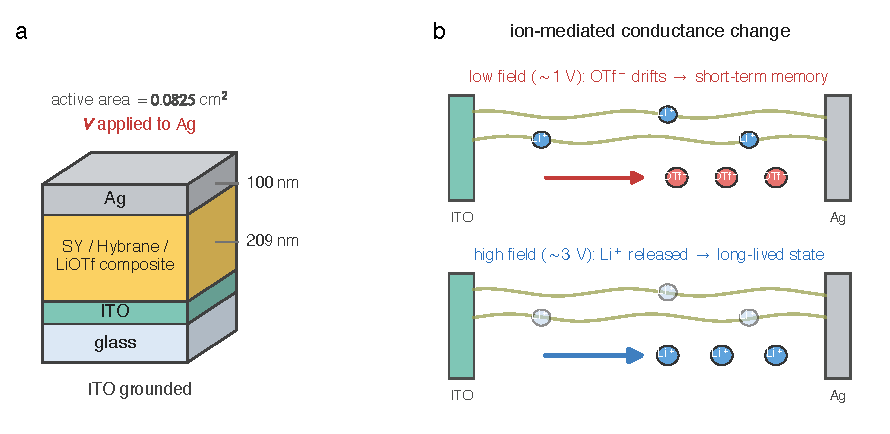
\includegraphics[width=\linewidth]{../figures/chapter2/device_schematic.pdf}
  \caption[Two-terminal device architecture]{Schematic of the two-terminal vertical synaptic device and active-layer mechanism. The device stack is ITO-glass / \SY{}/\Hybrane{}/\LiTf{} composite / Ag; the composite separates the electronic pathway, ion-transport host, and mobile-ion supply. The proposed mechanism assigns the faster STM response to weakly coordinated triflate redistribution and the longer-lived state to displacement of strongly coordinated \ce{Li+}. Schematic generated from the device geometry and mechanism reported in Ref.~\cite{PradoSocorro2022}.}
  \label{fig:device_schematic}
\end{figure}

The 2-T choice matters for two reasons. First, it reduces fabrication complexity, given that the device is made by a sequence of only three depositions (ITO substrate, spin-coated active layer, evaporated metal), which makes the same stack compatible with the comparative corpus of \Cref{ch:comparative}. Second, a 2-T device that shows coexisting \STM{} and \LTM{} without an independent gating signal shows that the memory physics is intrinsic to the active material, rather than being supplied externally by a gate field acting on a separate channel.

The bottom electrode is a pre-patterned layer of \ITO{} deposited on borosilicate glass. ITO combines optical transparency with adequate electronic conductance ($\sigma \approx \SI{e4}{\siemens\per\centi\metre}$)~\cite{Kim1999}, allowing optical inspection of the active layer and characterisation of the device stack by techniques such as UV-Vis spectroscopy and electroluminescence imaging. The work function of ITO ($\Phi_{\mathrm{ITO}} \approx \SI{4.7}{\electronvolt}$) is well matched to the ionisation potential of PPV-family semiconductors~\cite{Ramsdale2002}, facilitating hole injection into the active layer.

The top electrode is silver (Ag), deposited by thermal evaporation. Ag was selected over gold for reasons of cost and practical feasibility; its work function ($\Phi_{\mathrm{Ag}} \approx \SI{4.3}{\electronvolt}$) creates a modest electron injection barrier with the \SY{} conduction band, consistent with asymmetric injection conditions often observed in LEC-type structures~\cite{deMello1998}. The junction active area defined by the shadow mask geometry is \SI{0.0825}{\square\centi\metre}.

\subsection{Fabrication and Active-Layer Morphology}\label{subsec:fabrication_morphology}

ITO-patterned glass substrates were cleaned by sequential ultrasonication, dried under nitrogen, and transferred into a nitrogen glovebox. The composite solution was spin-coated at \SI{2000}{\rpm} for \SI{60}{\second} and annealed at \SI{75}{\celsius} for \SI{3}{\hour}. Contact profilometry gave an active-layer thickness of \SI{209}{\nano\metre} at this spin speed, and tapping-mode AFM showed smooth films with RMS roughness in the range \SIrange{1}{3}{\nano\metre} across the investigated processing window~\cite{PradoSocorro2022}. The spin-speed optimisation, profilometry method, AFM parameters, and supporting morphology evidence are reported in \chTwoSIRef{app:ch2_morphology_stability}.

The top electrode was \SI{100}{\nano\metre} of Ag deposited by thermal evaporation through a shadow mask. The mask defines a junction area of \SI{0.0825}{\square\centi\metre}. Detailed cleaning and evaporation parameters are collected in \chTwoSIRef{app:ch2_materials_fabrication}; the main point for the chapter is that the complete stack is fabricated by solution processing plus one metal evaporation step.


%% ------------------------------------------------------------
\section{Electrical Characterisation}\label{sec:elec_char}
%% ------------------------------------------------------------

Electrical measurements used a Keithley 2450 SourceMeter in a custom probe station. Unless otherwise stated, measurements were made under nitrogen with voltage applied to the Ag top electrode relative to grounded ITO. Protocol-level details are given in \chTwoSIRef{app:ch2_electrical_protocols}.

The characterisation is organised into two groups, following the distinction drawn in \cref{sec:ch2_intro}. \Cref{subsec:iv_hyst,subsec:pulse_potentiation,subsec:stm_ltm} report the three dynamical measurements that are carried forward to the comparative corpus of \Cref{ch:comparative,ch:temporal} --- current--voltage hysteresis, variable-number-of-pulses potentiation, and variable-delay depotentiation. \Cref{subsec:epsc,subsec:stdp} then report the extended synaptic protocols --- the EPSC multi-state readout and spike-timing dependent plasticity --- which are specific to this device and are not propagated to the later chapters. The short- and long-term memory regimes (\STM{}/\LTM{}) are obtained as an interpretation of the variable-delay depotentiation measurement, and are therefore presented together with it in \cref{subsec:stm_ltm}.

\subsection{Current-Voltage Hysteresis}\label{subsec:iv_hyst}

The fundamental electrical fingerprint of a memristive device is a current-voltage ($I$--$V$) hysteresis loop with a characteristic pinched appearance at zero voltage~\cite{Chua1971, Adhikari2013, Chua2014}. This shape arises because, at $V = 0$, the net current is zero regardless of the history of the device (a memristor cannot spontaneously drive current), yet the \textit{slope} of the $I$--$V$ curve at zero voltage (i.e., the instantaneous conductance) depends on the history of applied voltage.

\Cref{fig:iv_hyst} shows the $I$--$V$ curves obtained by applying successive triangular voltage sweeps to the device at a sweep rate of \SI{0.25}{\volt\per\second}, with the voltage ramped from \SI{0}{\volt} to a maximum of \SI{+1.2}{\volt} and back to \SI{0}{\volt} (single polarity, positive). A waiting period of \SI{10}{\second} was observed between successive sweeps to allow partial ionic relaxation. Ten sequential sweeps are shown.

\begin{figure}[htbp]
  \centering
  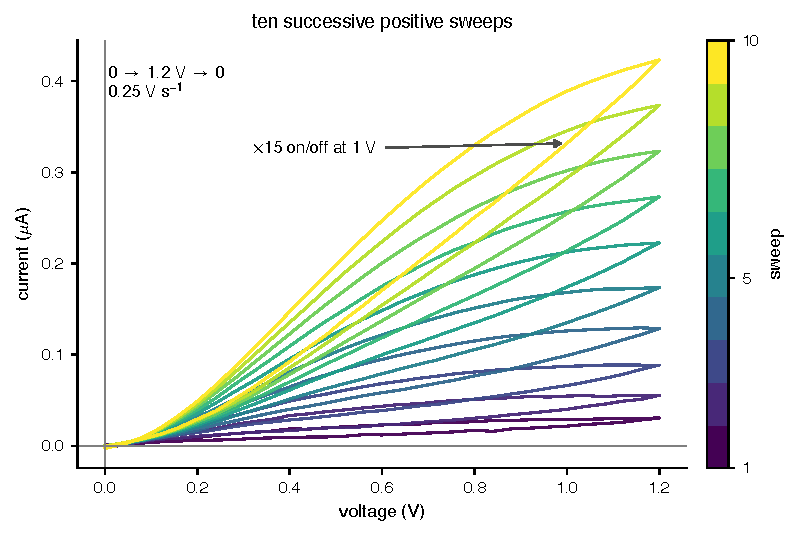
\includegraphics[width=0.86\linewidth]{../figures/chapter2/iv_hyst.pdf}
  \caption[Current--voltage hysteresis]{Current--voltage hysteresis of the composite memristive device. Ten successive positive triangular sweeps (\SIrange{0}{1.2}{\volt}, \SI{0.25}{\volt\per\second}, \SI{10}{\second} between cycles) show a progressive increase of conductance; the current at \SI{1}{\volt} rises by \SI{140}{\percent} from cycle~1 to cycle~2. The clockwise loop closes at the origin (pinched hysteresis) without abrupt switching. Data from Ref.~\cite{PradoSocorro2022}.}
  \label{fig:iv_hyst}
\end{figure}

Several features of these curves are noteworthy:

\paragraph{Progressive increase of conductance.} The current at any fixed voltage \textit{increases} with each successive sweep. From the first to the second cycle, the current at \SI{1}{\volt} increases by \SI{140}{\percent}. By the tenth cycle, the incremental increase from cycle 9 to cycle 10 is \SI{6.3}{\percent} — suggesting that the system is approaching a saturation conductance level asymptotically. This behaviour reflects the progressive redistribution of ions toward the electrodes with each sweep: each successive cycle leaves the ions in a slightly more asymmetric configuration than the previous one, producing a slightly lower resistance state.

\paragraph{Hysteresis without current rectification.} In all cycles, the return sweep (decreasing voltage) produces lower current than the forward sweep (increasing voltage) at the same voltage, generating the characteristic clockwise hysteresis loop for positive voltage sweeps. This is distinct from simple rectification (diode behaviour): a diode would produce the same forward and reverse $I$--$V$ curves; the hysteresis here reflects a time-dependent internal state variable (the ionic configuration) that lags the applied voltage.

\paragraph{Absence of abrupt switching.} Unlike digital resistance switching (SET/RESET transitions), in which the resistance changes abruptly by orders of magnitude at a threshold voltage, the conductance here evolves continuously and smoothly with each cycle. This \textit{analogue} gradation matters for the synaptic role outlined in \cref{subsec:why_hw}, since it allows the device state to be tuned to one of many distinguishable intermediate levels rather than being confined to two (or a few) binary states.

\paragraph{Behaviour under negative polarity.} Application of negative voltage sweeps (not shown individually in the main figure) produces a qualitatively different hysteresis: the current decreases rather than increases with successive negative cycles. This has been attributed to electrochemical side-reactions in the vicinity of the ITO electrode under large negative bias, which generate a thin insulating layer at the ITO/active layer interface analogous to the behaviour reported in MEH-PPV-based LECs~\cite{Wagberg2008, Fang2008}. This effect is not detrimental to memristive operation when devices are used in the single-polarity positive regime.

\subsection{Variable-Number-of-Pulses Potentiation}\label{subsec:pulse_potentiation}

Potentiation by a train of write pulses is the second of the three dynamical measurements introduced at the start of this section. Two complementary experiments are reported: a reversible potentiation/depression cycle that establishes the analogue, multi-state character of the conductance, and a measurement of the conductance change as a function of the number of applied pulses.

\subsubsection{Reversible Potentiation and Depression}

The ability to set the device conductance to a specific value by applying a controlled number of voltage pulses — and to subsequently decrease it back toward the initial value by pulses of opposite polarity — is demonstrated by the potentiation/depression experiment shown in \cref{fig:potentiation}.

A pulsed voltage protocol was applied: 50 consecutive write pulses of \SI{+1}{\volt} amplitude and \SI{0.1}{\second} duration, followed by 50 write pulses of \SI{-2}{\volt}. The conductance was monitored at the peak of each pulse (i.e., at the \SI{+1}{\volt} and \SI{-2}{\volt} levels, respectively). This protocol is analogous to the repeated pre-synaptic stimulation of a biological synapse and its subsequent inhibition.

The results demonstrate that the conductance can be continuously potentiated from its initial value by more than \SI{200}{\percent} during the \SI{+1}{\volt} pulse train, and subsequently depotentiated back toward the initial value during the \SI{-2}{\volt} train. The potentiation and depression curves are smooth and monotonic, without any abrupt transitions. The full reversibility of the process — the conductance returns to a value near the initial level after the complete depression protocol — confirms that the underlying ionic redistribution is non-destructive and does not permanently alter the chemical composition or morphology of the active layer.

The energy cost of each synaptic event (one write pulse of \SI{1}{\volt}, \SI{0.1}{\second}) can be estimated from the average current during the pulse. The resulting energy per event is approximately \SI{50}{\nano\joule}, or approximately \SI{6}{\femto\joule\per\micro\metre\squared} of device area (the \SI{0.0825}{\square\centi\metre} junction). This value is consistent with those reported for organic synaptic devices operating in the picojoule-to-nanojoule range~\cite{Xiao2016}, and comparable to the picojoule-to-nanojoule switching energies reported for inorganic memristive devices~\cite{YangStrukovStewart2013}.

\subsubsection{Quantitative Pulsed Read--Write Protocol}

To quantify the potentiation as a function of pulse number, and to separate the act of writing from the act of reading, a non-perturbing read protocol was adopted; the same protocol is reused for the depotentiation measurement of \cref{subsec:stm_ltm}. The read--write--wait sequence, detailed in \chTwoSIRef{app:ch2_read_write_wait}, comprises three steps:
\begin{enumerate}
  \item \textbf{Read.} A reading pulse ($V_{\mathrm{read}} = \SI{0.5}{\volt}$) is applied to establish the initial conductance $G_0$. This reading voltage is intentionally low: the activation threshold for ionic redistribution in this system was determined by independent experiments to lie above \SI{0.7}{\volt}~\cite{PradoSocorro2022}, so $V_{\mathrm{read}} = \SI{0.5}{\volt}$ measures the conductance state without perturbing it.
  \item \textbf{Write.} A train of $N_{\mathrm{pulses}}$ write pulses ($V_{\mathrm{write}}$, duration \SI{0.1}{\second} each) is applied.
  \item \textbf{Wait and read.} After a waiting time $t_{\mathrm{wait}}$ under open-circuit (high-impedance) conditions, a second reading pulse is applied to measure the final conductance $G_f$.
\end{enumerate}
The conductance change is reported as the percentage ratio $\Delta G = (G_f/G_0) \times 100$.

Between experiments, the device is fully reset by connecting the junction to a short circuit for \SI{300}{\second}, which discharges the ionic double layers and restores the homogeneous equilibrium ion distribution. The suitability of this reset protocol was verified by confirming that $G_0$ returns to its original value within the measurement uncertainty before each new experiment.

\subsubsection{Potentiation as a Function of Pulse Number}

\Cref{fig:npulse} shows the dependence of $\Delta G$ on $N_{\mathrm{pulses}}$ for $V_{\mathrm{write}} = \SI{1}{\volt}$ and $t_{\mathrm{wait}} = \SI{150}{\milli\second}$. The conductance ratio increases monotonically with $N_{\mathrm{pulses}}$, reaching values in excess of $10^3$\% for $N_{\mathrm{pulses}} > 10^3$. The relationship is approximately linear in log-log space for $N_{\mathrm{pulses}} < 100$ and saturates at large pulse numbers, consistent with a scenario in which the degree of ionic asymmetry that can be built up under a given write voltage is bounded by the total number of mobile ionic carriers.

\begin{figure}[htbp]
  \centering
  \begin{subfigure}[t]{0.48\linewidth}
    \centering
    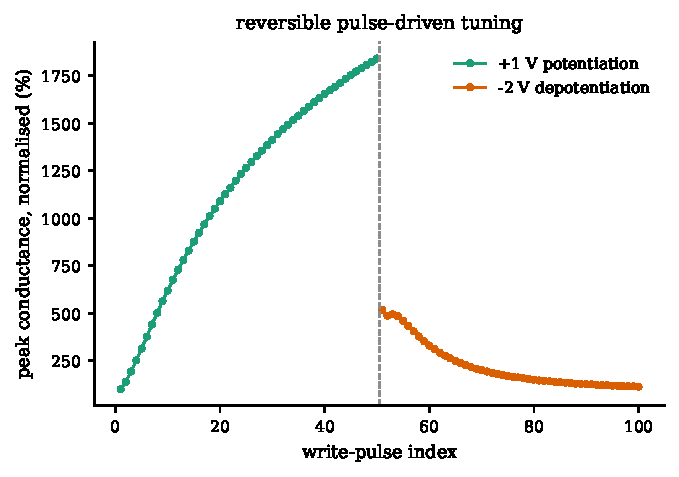
\includegraphics[width=\linewidth]{../figures/chapter2/potentiation_depression.pdf}
    \caption{Reversible potentiation/depression.}
    \label{fig:potentiation}
  \end{subfigure}\hfill
  \begin{subfigure}[t]{0.48\linewidth}
    \centering
    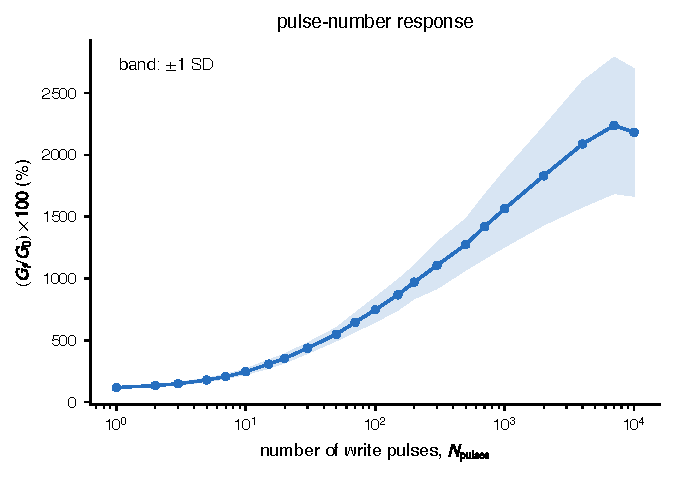
\includegraphics[width=\linewidth]{../figures/chapter2/pulse_number.pdf}
    \caption{Pulse-number response.}
    \label{fig:npulse}
  \end{subfigure}
  \caption[Pulse-driven conductance integration]{Pulse-driven conductance integration in the composite memristive device. \textbf{(a)} Fifty consecutive \SI{+1}{\volt} write pulses continuously potentiate the conductance; subsequent \SI{-2}{\volt} pulses depotentiate it toward the initial state. \textbf{(b)} Dependence of the conductance ratio \((G_f/G_0)\times100\%\) on the number of write pulses for \(V_{\mathrm{write}}=\SI{1}{\volt}\) and \(t_{\mathrm{wait}}=\SI{150}{\milli\second}\). The shaded band is one standard deviation across five independent crossbar pixels on the NM\_v055 substrate. Data regenerated from the local archive associated with Ref.~\cite{PradoSocorro2022}.}
  \label{fig:pulse_integration}
\end{figure}

Within this archived pulse-train dataset, the low-pulse-count response is reproducible to approximately the \SI{10}{\percent} level: for the five independent pixels in \cref{fig:npulse}, the median relative standard deviation is \SI{8.9}{\percent} and the largest value is \SI{11.8}{\percent} over the points with $N_{\mathrm{pulses}} < 100$. The dispersion increases modestly at large pulse numbers, reflecting the probabilistic nature of the ionic migration dynamics at large driving forces.

\subsection{Variable-Delay Depotentiation: Short- and Long-Term Retention}\label{subsec:stm_ltm}

The third dynamical measurement carried through the thesis probes how a written conductance state fades once the drive is removed: the depotentiation of the device measured as a function of the delay before read-out. This is one of the most important characterisation protocols for neuromorphic devices, because it determines whether the device can emulate short-lived and longer-lived synaptic states on experimentally accessible timescales. In the artificial-synapse literature these regimes are commonly labelled \STM{} and \LTM{}; in the present system, the longer-lived regime remains on the sub-minute scale and should therefore be understood operationally rather than as a claim of indefinitely persistent storage.

The measurement reuses the pulsed read--write protocol of \cref{subsec:pulse_potentiation}, with the waiting time $t_{\mathrm{wait}}$ now the swept variable and the pulse number held fixed. \Cref{fig:retention} shows the dependence of $\Delta G$ on $t_{\mathrm{wait}}$ for three excitation conditions: (i) $V_{\mathrm{write}} = \SI{1}{\volt}$, $N_{\mathrm{pulses}} = 10$ (STM, blue); (ii) $V_{\mathrm{write}} = \SI{1}{\volt}$, $N_{\mathrm{pulses}} = 50$ (STM, red); and (iii) $V_{\mathrm{write}} = \SI{3}{\volt}$, $N_{\mathrm{pulses}} = 10$ (LTM, black).

\begin{figure}[htbp]
  \centering
  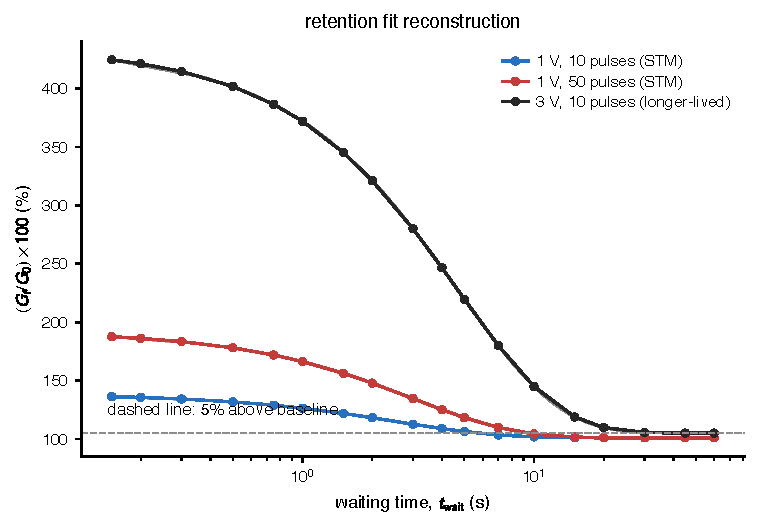
\includegraphics[width=0.82\linewidth]{../figures/chapter2/retention.pdf}
  \caption[Memory retention kinetics]{Memory retention kinetics. Conductance ratio $(G_f/G_0)\times 100\%$ versus waiting time $t_{\mathrm{wait}}$ for STM conditions (\SI{1}{\volt}; 10 and 50 pulses, blue/red) and the longer-lived regime denoted LTM (\SI{3}{\volt}, 10 pulses, black). Solid lines are standard-exponential reconstructions of the form in \cref{eq:retention_exp}; the fit parameters are summarised in \chTwoSIRef{app:ch2_retention_fits}. Data and fit parameters from Ref.~\cite{PradoSocorro2022}.}
  \label{fig:retention}
\end{figure}

For short waiting times ($t_{\mathrm{wait}} < \SI{500}{\milli\second}$ for STM conditions, $t_{\mathrm{wait}} < \SI{2}{\second}$ for LTM conditions), the conductance first \textit{increases} slightly relative to the value immediately after the write pulse train. This counterintuitive behaviour is \emph{not} ascribed to ionic inertia: ion transport in the polymer matrix is strongly overdamped, so any momentum imparted by the field relaxes on a timescale orders of magnitude shorter than the observed enhancement. It is instead attributed to the continued redistribution of ions after the drive is removed. At the end of the pulse train the ionic configuration and its self-consistent space-charge field have not yet reached their quasi-steady profile; the residual internal field, together with the slow advance of the electrochemically doped region near the electrode, continues to raise the conductance for a brief interval before the diffusion-driven relaxation sets in. An analogous transient enhancement following a stimulus train has been described as ``post-tetanic potentiation'' in biological synaptic preparations~\cite{Zucker1989, ZuckerRegehr2002}.

For longer waiting times, the expected exponential relaxation of conductance is observed as the ionic configuration relaxes back toward equilibrium by thermal diffusion. The fit record summarised in \chTwoSIRef{app:ch2_retention_fits} reports least-squares fits in IGOR Pro 8 to a standard exponential:

\begin{equation}
  \frac{G_f(t_{\mathrm{wait}})}{G_0} = R_\infty + A \exp\!\left(-\frac{t_{\mathrm{wait}}}{\tau}\right)
  \label{eq:retention_exp}
\end{equation}

where $\tau$ is the characteristic relaxation time, $A$ is the decaying amplitude, and $R_\infty$ is the long-waiting-time conductance ratio. In other words, the published proof-of-concept fit corresponds to a stretched-exponential model with the stretch exponent fixed at $\beta=1$. No free $\beta$ parameter, confidence interval, or goodness-of-fit statistic was reported for these three traces, so the \cref{ch:poc} evidence is used here only to establish the two experimentally resolved relaxation times, not to claim a fitted distribution of relaxation barriers. The later comparative analysis in \cref{ch:comparative} uses a free-exponent Kohlrausch descriptor only where the DELAYTIME archive is refitted consistently across the comparative corpus.

The fitted characteristic times are $\tau_S = \SI{2.57}{\second}$ for the \SI{1}{\volt}, 10-pulse STM trace, $\tau_S = \SI{3.01}{\second}$ for the \SI{1}{\volt}, 50-pulse STM trace, and $\tau_L = \SI{4.73}{\second}$ for the \SI{3}{\volt}, 10-pulse LTM trace. The corresponding offsets and amplitudes are tabulated in \chTwoSIRef{app:ch2_retention_fits}. The retention time --- defined operationally as the waiting time at which $G_f/G_0$ returns to within \SI{5}{\percent} of the baseline (i.e., $G_f/G_0 < 1.05$) --- is \SIrange{10}{15}{\second} for STM and exceeds \SI{45}{\second} for the longer-lived regime labelled LTM. These values are directly relevant to the timescales of spike-based computation: the \SIrange{10}{15}{\second} STM window is sufficient to maintain working memory over a series of sequential spike inputs, while the $> \SI{45}{\second}$ LTM window shows that the device can preserve a write history over many subsequent events without approaching the retention regime of a conventional non-volatile memory.

The molecular mechanism underlying the STM/LTM distinction is discussed in detail in \cref{sec:mechanism}.

\subsection{Excitatory Post-Synaptic Current}\label{subsec:epsc}

The \EPSC{} measurement is a standard protocol in the field of artificial synaptic devices, designed to quantify the number and stability of distinguishable conductance states accessible to the device~\cite{Kim2018, VanDeBurgt2018}. The protocol employed here closely mimics the biological experiment in which a patch-clamped neuron is subjected to a defined sequence of pre-synaptic inputs and the post-synaptic current is monitored.

The measurement protocol is as follows (\cref{fig:epsc}):
\begin{enumerate}
  \item \textbf{Initialisation.} The device is initialised to its ground state $S_0$ by applying a fixed read-out bias $V_0 = \SI{+1}{\volt}$ for \SI{1}{\second}. This bias differs in purpose from the sub-threshold probe ($V_{\mathrm{read}} = \SI{0.5}{\volt}$) used for the non-perturbing read-out of \cref{subsec:pulse_potentiation,subsec:stm_ltm}: the EPSC states are defined operationally by the current response at a single common read-out bias against which all states $S_0$--$S_4$ are referenced, not by a passive probe required to leave the state untouched.
  \item \textbf{Excitation.} A short positive write pulse of \SI{+2}{\volt} for \SI{50}{\milli\second} is applied; the device is subsequently held at \SI{+1}{\volt} for \SI{1}{\second}, during which the conductance spontaneously relaxes to a new excited steady state $S_1$. The same sequence is repeated to produce a second excited state $S_2$.
  \item \textbf{Inhibition.} Two negative write pulses of \SI{-2.5}{\volt} for \SI{50}{\milli\second} are applied, producing inhibitory states $S_3$ and $S_4$.
\end{enumerate}

The four excited states are readily distinguishable from each other and from the ground state. Defining the \EPSC{} readout ratio $R_n = I_{S_n}/I_{S_0}$ as the signed current response of state $S_n$ normalised to that of the ground state $S_0$ under the fixed read-out bias used in the experiment, the values obtained are: $R_1 = 7.33$, $R_2 = 15.55$, $R_3 = -3.72$, $R_4 = -16.97$. (The ratio is formed from signed currents rather than conductances, so the inhibitory states carry a negative sign; conductance itself remains non-negative throughout.) The large absolute ratios (up to $\sim$16-fold increase or $\sim$17-fold decrease relative to $S_0$) provide a wide margin for reliable state identification in a practical device, even in the presence of noise. The four-state sequence used here is a representative demonstration rather than an upper bound: given the continuous, analogue conductance tunability established in \cref{subsec:pulse_potentiation}, the number of distinguishable readout states is not intrinsically limited to four, and many more intermediate levels could in principle be resolved by the same protocol within the available margin.

The states \(S_1\) and \(S_2\) are reached by \textit{excitatory} (positive polarity) stimulation, while \(S_3\) and \(S_4\) are reached by \textit{inhibitory} (negative polarity) stimulation, in direct analogy with long-term potentiation (LTP) and long-term depression (LTD) at biological synapses. The coexistence of both excitatory and inhibitory states in the same 2-T device, without an independent gate terminal, distinguishes the present platform from the 3-T organic implementations discussed in \cref{subsec:organic_precedents}.

\subsection{Spike-Timing Dependent Plasticity}\label{subsec:stdp}

Spike-timing dependent plasticity is a timing-dependent Hebbian learning rule: it instantiates Hebb's local correlation principle~\cite{Hebb1949} in a form that was later observed experimentally in biological preparations~\cite{Markram1997, Bi1998}. Here the timing delay is defined as \(\Delta t = t_{\mathrm{post}} - t_{\mathrm{pre}}\). With this convention, if the presynaptic neuron fires shortly \textit{before} the postsynaptic neuron (causal ordering, $\Delta t < 0$), the synapse is potentiated (LTP); if the presynaptic neuron fires shortly \textit{after} the postsynaptic neuron (anti-causal ordering, $\Delta t > 0$), the synapse is depressed (LTD). The magnitude of the change decays exponentially with $|\Delta t|$. This temporal asymmetry is essential for the synaptic encoding of causal relationships in neural circuits and underlies the ability of STDP-based learning rules to implement unsupervised feature extraction and pattern recognition~\cite{Bichler2012}.

\subsubsection{Experimental Protocol}

The STDP experiment requires the emulation of pre- and postsynaptic spike waveforms by voltage pulses applied at the two electrodes of the device. In a 2-T device, both pulses must be applied at the same physical terminal (the Ag electrode), so the experimentally measured total voltage $V(t)$ is the algebraic sum of the presynaptic and postsynaptic voltage waveforms separated by the delay $\Delta t$:

\begin{equation}
  V(t) = V_{\mathrm{pre}}(t) + V_{\mathrm{post}}(t + \Delta t)
  \label{eq:stdp_voltage}
\end{equation}

Each spike waveform consists of a unipolar triangular pulse with maximum amplitude $V_{sp}$ and duration \SI{1.2}{\second}. The delay $\Delta t$ was varied from \SI{-600}{\milli\second} to \SI{+600}{\milli\second}. The amplitude $V_{sp} = \SI{1.55}{\volt}$ was chosen to be large enough to activate ionic migration (above the threshold of approximately \SI{0.7}{\volt}) while remaining below the onset of electrochemical degradation of the active layer (conservatively estimated at \SI{2}{\volt} for the pristine device).

For \(\Delta t < 0\) (pre fires before post), the two spike waveforms partially overlap in time with additive polarity, producing a composite pulse whose peak voltage exceeds \(V_{sp}\) and which is directed in the positive sense. The ions then redistribute toward the ITO electrode, the conductance increases, and the device records a net synaptic potentiation.

For \(\Delta t > 0\) (post fires before pre), the overlap produces an anti-causal summation. Depending on the exact waveforms, the effective net voltage can be of reduced amplitude or of reversed polarity relative to the causal case, so the ionic redistribution is either weaker or reversed and the conductance decreases, in the form of a net synaptic depression.

\subsubsection{STDP Curve and Fitting}

\Cref{fig:stdp} shows the measured STDP function: the percentage conductance change $\Delta G$ plotted against the timing delay $\Delta t$. Under the sign convention above, the measured kernel is asymmetric Hebbian: negative $\Delta t$ (causal) produces positive $\Delta G$ (potentiation), and positive $\Delta t$ (anti-causal) produces negative $\Delta G$ (depression). Each branch (potentiation for $\Delta t < 0$, depression for $\Delta t > 0$) is fitted separately, as a function of the absolute delay $|\Delta t|$, by a decaying exponential:

\begin{equation}
  \Delta G(\Delta t) = A_{\pm}\,\exp\!\left(-\frac{|\Delta t|}{\tau_{\pm}}\right) + G_0
  \label{eq:stdp_fit}
\end{equation}

where $A_{\pm}$ and $\tau_{\pm}$ are the branch-specific amplitude and time constant ($+$ for the potentiation branch, $-$ for the depression branch) and $G_0$ is a constant offset. The best-fit values of $\tau_{\pm}$ for both the potentiation and depression branches lie in the range \SIrange{85}{90}{\milli\second}. This is in close quantitative agreement with the characteristic timescale of biological STDP, which is approximately \SI{100}{\milli\second}~\cite{Kuzum2013, Bi1998}. The device, therefore, not only qualitatively replicates the STDP function but does so with biologically realistic time constants.

\begin{figure}[htbp]
  \centering
  \begin{subfigure}[t]{0.48\linewidth}
    \centering
    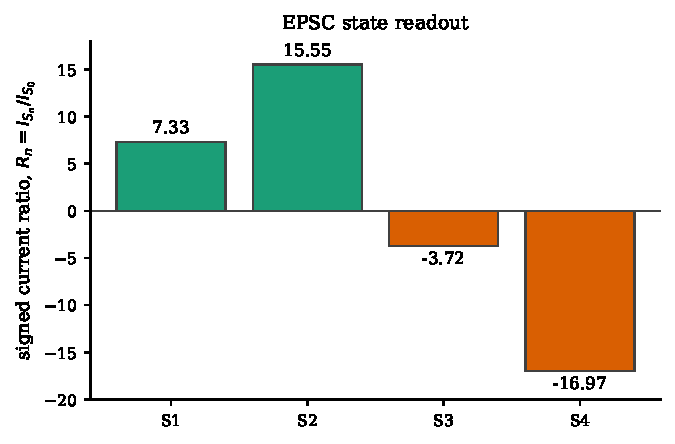
\includegraphics[width=\linewidth]{../figures/chapter2/epsc_summary.pdf}
    \caption{EPSC state ratios.}
    \label{fig:epsc}
  \end{subfigure}\hfill
  \begin{subfigure}[t]{0.48\linewidth}
    \centering
    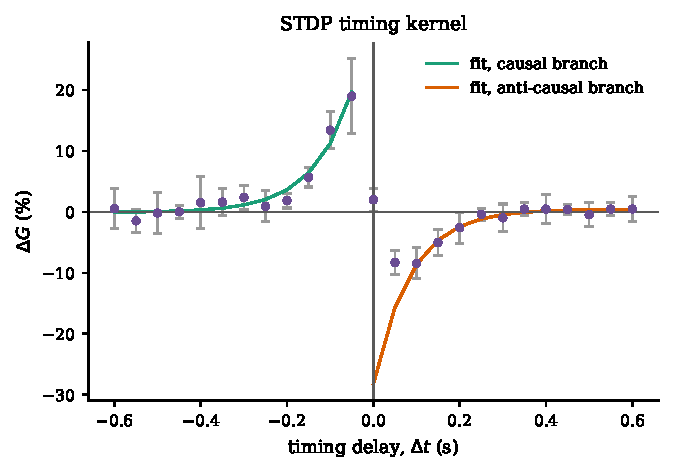
\includegraphics[width=\linewidth]{../figures/chapter2/stdp_summary.pdf}
    \caption{STDP timing kernel.}
    \label{fig:stdp}
  \end{subfigure}
  \caption[Compact EPSC and STDP summary]{Compact summary of the extended synaptic measurements. \textbf{(a)} Signed EPSC readout ratios \(R_n=I_{S_n}/I_{S_0}\) for the four demonstrated states. \textbf{(b)} Spike-timing dependent plasticity: percentage conductance change \(\Delta G\) as a function of the pre/post spike-timing delay \(\Delta t\), with each branch fitted to the decaying exponential of \cref{eq:stdp_fit}. Data and reported state ratios from Ref.~\cite{PradoSocorro2022}; STDP curve regenerated from the local NM\_v055 Day19 archive.}
  \label{fig:extended_synapse_summary}
\end{figure}

The result that the obtained learning rule corresponds to \textit{asymmetric Hebbian} STDP reflects the specific voltage waveform design, the stated definition of \(\Delta t\), and the polarity conventions of the electrode configuration. Different waveform designs or an opposite sign convention would be expected to produce differently labelled STDP kernels, offering an additional degree of tunability in the design of hardware neural network architectures built from these devices.


%% ------------------------------------------------------------
\section{Theoretical Framework: Ion Transport and the Origin of Memristance}\label{sec:mechanism}
%% ------------------------------------------------------------

The injection and bulk-transport physics of the composite are described by two limiting-case models inherited from the polymer light-emitting electrochemical cell (LEC) literature: an \emph{electrodynamic} (injection-limited) model~\cite{deMello1998,deMello2002} and an \emph{electrochemical-doping} (ohmic) model~\cite{Pei1995,Smith1997,Matyba2009}, which van~Reenen \textit{et al.}~\cite{vanReenen2010} reconciled as two regimes of the same field-driven ion redistribution. The equilibrium ion distribution, the thermionic-injection description, and the two models in full are set out in \chTwoSIRef{app:ch2_ion_models}; the focus here is on what they imply for the two observed memory regimes.

For the present SY/Hybrane/LiOTf system, the \SY{} polymer has moderate hole mobility and a moderate injection barrier from ITO, so both mechanisms may contribute simultaneously. The interpretation adopted here associates the ED mechanism with the rapid conductance changes at short timescales (milliseconds to seconds), driven primarily by the fast-moving triflate anions, and the ECD mechanism with the larger, slower changes at longer timescales (seconds to tens of seconds), driven by the slower-moving \ce{Li+} cations; on this reading the hierarchy of timescales is the physical origin of the STM/LTM dichotomy. It should be stressed that the device-level measurements of \cref{sec:elec_char} do not by themselves uniquely separate the two contributions: a clean discrimination would require, for instance, their temperature, film-thickness, or sweep-rate dependence, which is not pursued here. The assignment is therefore a working interpretation rather than an established fact. Its central falsifiable consequence --- that the slow timescale should track the cation--host coordination strength --- is examined directly in \Cref{ch:comparative} by varying the cation at fixed host chemistry.

\subsection{Lewis Acid-Base Chemistry and the Two Memory Regimes}\label{subsec:lewis}

The chemical mechanism proposed here for the two memory regimes is the same hard--soft acid--base reasoning developed in \cref{subsec:ion_conducting_polymers,subsec:composite_rationale}, applied to the specific salt and host of this device.

Within the HSAB framework, the strength of the interaction between a Lewis acid and a Lewis base in a coordination environment is set by the matching of their hardness or softness~\cite{Pearson1963}. The hard--hard interaction between \ce{Li+} (a small, hard Lewis acid with charge density \(z/r \approx\) \SIrange{1.3}{1.7}{\per\angstrom}) and the ether oxygen atoms of \Hybrane{} (hard Lewis bases) is governed predominantly by electrostatic forces, and is therefore thermodynamically strong and geometrically specific. In polyether environments \ce{Li+} is coordinated by four to six oxygen donors --- five in the crystalline complex \(\mathrm{PEO_3{:}LiCF_3SO_3}\) (three ether oxygens and two triflate oxygens) --- with oxygen--lithium distances of \SIrange{1.9}{2.1}{\angstrom}~\cite{Lightfoot1993}. This local site \emph{binding} should not be confused with the \emph{migration} activation barrier that governs hopping: the latter is the saddle-point barrier between adjacent sites --- of order \SI{50}{\kilo\joule\per\mol} ($\approx 20\,k_{\mathrm{B}}T$; \cref{subsec:hybrane}) --- and is therefore smaller than the full coordination well, while still being substantially larger than \(k_{\mathrm{B}}T\).

The interaction between the \ce{CF3SO3-} triflate anion and the host oxygens is, by contrast, much weaker. The diffuse, low-charge-density triflate anion does not engage in strong electrostatic interactions with the hard-base oxygen atoms, and the residual interaction is governed mainly by weak van der Waals forces~\cite{BruceVincent1993,Frech1999PEOLiTf}. The energy barrier for displacement of a triflate anion from one interstitial site to the next is therefore expected to be substantially lower than the barrier for a \ce{Li+} cation.

This differential activation barrier translates directly into a differential ionic mobility under an applied field, and hence into different voltage thresholds for significant ionic redistribution:

\begin{itemize}
  \item A modest voltage of \SI{1}{\volt} applied across a \SI{209}{\nano\metre} film generates a field of approximately \SI{4.8}{\mega\volt\per\metre}. In the interpretation adopted here, this is sufficient to drive the more weakly bound triflate-anion redistribution observed experimentally~\cite{PradoSocorro2022}. The fast anionic redistribution produces a rapid conductance change, which then relaxes on the timescale of triflate diffusion through the host. This is the \STM{} regime, with retention \SIrange{10}{15}{\second}, driven primarily by triflate relaxation.

  \item A voltage of \SI{3}{\volt} across the same film generates approximately \SI{14.4}{\mega\volt\per\metre}. This higher field is assigned to the onset of a slower cation contribution, consistent with the stronger \ce{Li+} coordination expected in oxygen-rich polyether hosts~\cite{Lightfoot1993,BruceVincent1993}. The cation contribution sets in, produces a delayed and stronger ionic redistribution, and relaxes on the much longer timescale of cation re-coordination. This is the \LTM{} regime, with retention exceeding \SI{45}{\second}, driven primarily by cation redistribution.
\end{itemize}

This account yields a specific, experimentally testable prediction. Replacing \ce{Li+} with a monovalent cation of larger ionic radius (\ce{Na+} or \ce{K+}) should reduce the charge density, and therefore the hardness, of the Lewis acid. The cation--oxygen coordination with the polyether host should weaken accordingly, and the slow fading-memory timescale of the device should shorten as the cation is moved along the \ce{Li+} \(\to\) \ce{Na+} \(\to\) \ce{K+} series. The prediction is tested in \Cref{ch:comparative} on the main comparative corpus of the thesis: a PEO-based polymer-electrolyte series loaded with lithium, sodium and potassium triflate salts (PEO/LiOTf, PEO/NaOTf, PEO/KOTf) at fixed polymer and salt mass fractions, complemented by a dedicated PEO/LiOTf concentration sub-study. The prediction is addressed there as a statement about the shift of the measured variable-delay depotentiation timescale when the cation is varied at fixed host chemistry, not as a claim about the full synaptic suite reported in the present chapter.


%% ------------------------------------------------------------
\section{Device Stability and Reproducibility}\label{sec:stability}
%% ------------------------------------------------------------

\subsection{Ambient Shelf Stability}\label{subsec:lifetime}

Two distinct notions of device longevity must be kept separate. \emph{Cycling endurance} --- the number of write/erase cycles a device sustains before its performance parameters drift outside specified tolerances --- is the metric that ultimately governs suitability for the millions-to-billions of weight updates of on-chip training; it is not characterised for the present devices and is left for future work. \emph{Shelf (calendar) stability} --- the retention of performance during storage and intermittent operation under ambient conditions --- is what is reported here. It is the more immediately relevant metric at the proof-of-concept stage, where the question is simply whether the unencapsulated composite survives realistic handling at all.

The devices reported here were characterised at regular intervals over a period of two weeks (\SI{{\sim}300}{\hour}) after fabrication, without encapsulation, while stored in ambient air at room temperature. The key metrics monitored were the baseline conductance $G_0$, the maximum achievable conductance change $\Delta G_{\mathrm{max}}$, and the STM retention time $\tau_S$; the supporting stability record is collected in \chTwoSIRef{app:ch2_morphology_stability}.

The results show that all three metrics remain within \SI{20}{\percent} of their initial values over the full two-week measurement period~\cite{PradoSocorro2022}. This stability compares favourably with other organic memristive devices reported in the literature, which typically exhibit significant degradation within hours to days under ambient conditions~\cite{Shih2016}. The enhanced stability is attributed to the solid-state nature of the composite: unlike devices based on liquid electrolytes or gel polymers, the Hybrane matrix provides a mechanically cohesive environment that protects the ions from evaporation and the polymer films from delamination, consistent with the stability of related Hybrane-based LEC blends~\cite{Mardegan2021}.

\subsection{Device-to-Device Reproducibility}\label{subsec:reproducibility}

Reproducibility is a persistent challenge for memristive devices, particularly those based on filamentary switching in inorganic materials, where the stochastic nucleation of conducting filaments produces large device-to-device and cycle-to-cycle variability~\cite{Sun2019}. The present system, which operates by uniform bulk ionic redistribution rather than localised filament formation, is intrinsically less susceptible to this type of variability.

The strongest reproducibility statement available from the archived proof-of-concept data is the one attached to the pulse-number experiment in \cref{fig:npulse}. That dataset contains five independent crossbar pixels on the NM\_v055 substrate, measured under the same \SI{1}{\volt} write and \SI{150}{\milli\second} wait protocol. The shaded band is one standard deviation across those five pixels. For $N_{\mathrm{pulses}} < 100$, the median RSD is \SI{8.9}{\percent} and the largest RSD is \SI{11.8}{\percent}; the appropriate claim is therefore reproducibility at about the \SI{10}{\percent} level in the low-pulse-count regime, not an exact upper bound below \SI{10}{\percent}.

The EPSC readout and STDP measurements remain important protocol demonstrations, but the recovered archive does not contain a normalized EPSC population table comparable to the PULSES and DELAYTIME tables used later in the thesis. They are therefore not used to support an independent EPSC RSD claim here. Likewise, the published proof-of-concept data establish same-substrate/pixel reproducibility and two-week shelf stability; they should not be read as a powered batch-to-batch reproducibility study. Campaign-scale reproducibility --- a separate metric on a separate axis --- and its resolution by a change of ion-transport host are taken up in \cref{ch:bridge}.


%% ------------------------------------------------------------
\section{Comparison at the Time of Publication}\label{sec:comparison}
%% ------------------------------------------------------------

The historical comparison table reproduced in \chTwoSIRef{tab:ch2_historical_comparison} places this device alongside representative organic and hybrid memristive devices available at the time of the 2022 publication. Two combinations stand out as unrepresented in that set. The first is the coexistence of \STM{} and \LTM{} in a single \emph{fully reversible} 2-T device: the closest prior report, Liu \textit{et al.}~\cite{Liu2016}, achieved short-to-long-term transitions but through irreversible redox chemistry~\cite{Heremans2011}, whereas here the conductance returns to \(G_0\) after the reset protocol. The second is STDP in a 2-T architecture, where the timing rule emerges from the superposition of pre- and postsynaptic pulses at the single Ag terminal rather than from the gate of a 3-T device~\cite{Gkoupidenis2015,Kim2018,Seo2019}. On the operating-regime axes the device is competitive in unencapsulated shelf lifetime (\(\sim\)\SI{300}{\hour}, roughly an order of magnitude beyond comparable organic devices~\cite{Shih2016}) but not in energy per event (\(\sim\)\SI{50}{\nano\joule}, above CMOS and inorganic-memristor budgets~\cite{IndiveriLiu2015,YangStrukovStewart2013}); the full table and a per-axis discussion are given in \chTwoSIRef{app:ch2_comparison}.

The comparison above retains the device-level metrics conventional in the organic memristive literature of the early 2020s: reversibility, retention window, energy per event, and operational lifetime. Subsequent work has broadened the field substantially, particularly through organic electrochemical neurons and neuromorphic circuits~\cite{Harikesh2024OECNReview,Krauhausen2024Robotics} and through the wider organic-iontronic memristor landscape~\cite{Xia2024OIMReview}. The table is therefore used only to locate the 2022 proof-of-concept result historically. Within the thesis-wide argument, those metrics play a narrower role: they establish that the polymer-electrolyte platform introduced here is reversible, dynamically addressable, and stable enough to support the comparative study of \Cref{ch:comparative} (a PEO-based triflate composition and cation sweep, characterised through the same three common dynamical measurements) and the temporal-computing reinterpretation of \Cref{ch:temporal} built on those measurements. They are not invoked to claim that this device should be judged by the standards of a high-density non-volatile memory technology, nor to suggest that the full synaptic suite reported here is available across the full comparative corpus. Those measurements remain specific to the present SY/Hybrane/LiOTf device.


%% ------------------------------------------------------------
\section{Summary}\label{sec:ch2_summary}
%% ------------------------------------------------------------

This chapter has reported the design, fabrication, and characterisation of a fully reversible 2-T organic memristive device that supports, within a single polymer-composite active layer, a full set of synaptic functions organised in two families: the three dynamical measurements carried through the rest of the thesis (I--V hysteresis, variable-number-of-pulses potentiation, and variable-delay depotentiation), and the extended synaptic protocols specific to this device (EPSC, the separated \STM{}/\LTM{} reading of the retention data, and \STDP{}).

A ternary \SY{}/\Hybrane{}/\LiTf{} composite satisfies the three functional requirements of \cref{subsec:design_rationale} (electronic pathway, ion-transport medium, ion source), fabricated as a 2-T ITO/composite/Ag sandwich by solution processing and one evaporation step, with a \SI{209}{\nano\metre} active layer below \SI{3}{\nano\metre} RMS roughness. On this single platform the three dynamical measurements carried forward to the comparative corpus were established: analogue I--V hysteresis (a \SI{140}{\percent} conductance rise from cycle~1 to~2 at \SI{1}{\volt}); fully reversible pulse potentiation/depression exceeding \SI{200}{\percent} at \(\sim\)\SI{50}{\nano\joule} per event, growing past \(10^3\%\) for \(N_{\mathrm{pulses}}>10^3\); and variable-delay depotentiation resolving two regimes (\STM{}, \(\tau_S=\SIrange{2.57}{3.01}{\second}\), retention \SIrange{10}{15}{\second}; \LTM{}, \(\tau_L=\SI{4.73}{\second}\), retention \(>\SI{45}{\second}\), from $\beta=1$ fits). The extended single-device protocols add a four-state EPSC read-out (signed ratios \(-17\) to \(+16\)) and an asymmetric-Hebbian STDP window (\(\tau=\SIrange{85}{90}{\milli\second}\), biologically realistic~\cite{Bi1998,Kuzum2013}). The \STM{}/\LTM{} dichotomy is attributed to the Lewis acid--base mobility asymmetry between the weakly coordinated triflate anion and the strongly coordinated \ce{Li+} cation in the oxygen-rich host, with the injection and bulk-transport physics described by the electrodynamic and electrochemical-doping models in their reconciled form~\cite{vanReenen2010} (\chTwoSIRef{app:ch2_ion_models}). Devices were stable over a \(\sim\)\SI{300}{\hour} unencapsulated ambient shelf (cycling endurance not characterised), with \(\sim\)\SI{10}{\percent} low-pulse-count variability across five pixels on NM\_v055 (median RSD \SI{8.9}{\percent}); campaign-scale reproducibility is taken up in \cref{ch:bridge}.

Taken together, these results establish the SY/Hybrane/LiOTf composite as a thoroughly characterised exemplar of a polymer-electrolyte organic memristive device, and identify cation--polyether coordination chemistry as the physical hypothesis for memory-timescale control. This identification motivates the main comparative study of \Cref{ch:comparative}, which replaces \Hybrane{} with poly(ethylene oxide), varies the PEO/LiOTf composition as the replicated quantitative axis, and surveys host, anion, and cation substitutions as sample-limited chemical side evidence. In \Cref{ch:comparative}, the hypothesis is tested through the three common dynamical measurements (I--V hysteresis, variable-number-of-pulses potentiation, and variable-delay depotentiation) that are abundant across the comparative corpus; the outcome is deliberately cautious, with no robust host- and anion-independent Li/Na/K law claimed. The richer synaptic metrics reported in the present chapter (EPSC, separated \STM{}/\LTM{} retention, and STDP) are not propagated to the later chapters and serve there only as lithium-device priors and sanity checks. Beyond this comparative handoff, the volatile two-timescale behaviour established here is the experimental anchor for the temporal-computing reinterpretation of \Cref{ch:temporal}, in which behavioural models fitted to the \Cref{ch:comparative} corpus drive reservoir-computing simulations, physiological temporal-context reconstruction, and WESAD affective-computing demonstrations. In those paradigms, the fading memory of the device is the active computational resource rather than a retention defect to be suppressed.


%% ---- Standalone close (skipped when \include'd from thesis.tex) ----
%% A unified bibliography is printed from thesis.tex in the thesis build,
%% so the per-chapter \printbibliography runs only in standalone mode.
\ifdefined\thesismode
  \let\thesisstandaloneclose\relax
\else
  \printbibliography[heading=bibintoc, title={References}]
  \def\thesisstandaloneclose{\end{document}}
\fi
\thesisstandaloneclose

%% ============================================================
%%  Chapter (bridge) — Reproducibility, Degradation, and the
%%                     Device-Provenance Infrastructure
%%
%%  Author : Carlos David Prado-Socorro
%%  Date   : June 2026
%%  Institution : ICMol, Universitat de València
%%
%%  Compile with: latexmk -pdf  (standalone) or via thesis.tex
%%  Plan + evidence: handouts/22_bridge_chapter_plan.md,
%%                   scripts/bridge_hybrane_peo_reproducibility.py,
%%                   handouts/bridge_hybrane_peo_summary.csv
%% ============================================================

%% ---- Standalone preamble (skipped when \include'd from thesis.tex) ----
\ifdefined\thesismode\else
  \documentclass[12pt, twoside]{report}
  \usepackage{thesis-format}
  \addbibresource{../bibliography/references.bib}
  \begin{document}
  \setcounter{chapter}{2}     % This is Chapter 3 when built standalone
\fi

%% --- Shared macros (\providecommand: harmless if earlier chapters declared them) ---
\providecommand{\SY}{\textit{Super Yellow}}
\providecommand{\Hybrane}{\textit{Hybrane}}
\providecommand{\PEO}{PEO}
\providecommand{\LiTf}{LiOTf}
\providecommand{\ITO}{ITO}
\providecommand{\twoterminal}{two-terminal}
%% Standalone-safe reference into this chapter's Supporting Information
%% (Appendix B). Resolves with \cref in the full thesis; prints a literal
%% label in standalone builds, where the appendix is not included.
\providecommand{\siBridgeRef}[1]{\ifdefined\thesismode\cref{#1}\else Appendix~B\fi}

%% ============================================================
\chapter{Reproducibility, Degradation, and the Device-Provenance Infrastructure}\label{ch:bridge}
%% ============================================================

%% ------------------------------------------------------------
\section{The Reproducibility Problem}\label{sec:bridge_problem}
%% ------------------------------------------------------------

\Cref{ch:poc} established, on a single fully characterised \SY{}, \Hybrane{}, and \LiTf{} device, that a three-component polymer-electrolyte composite supports the complete set of memristive functions in one \twoterminal{} platform, and that the proof-of-concept device was stable on a two-week ambient shelf scale. \Cref{ch:comparative} will treat the volatile dynamics of these composites as something to be engineered across a replicated composition grid. Between those two results sits a problem that has to be confronted before the comparative study can be read on its own terms, and that is the subject of this short chapter: \emph{as the campaign scaled from a single validated device to a fabrication programme, the memristive hysteresis became progressively harder to obtain.} Successive batches of nominally identical \SY{}/\Hybrane{}/\LiTf{} devices drifted away from the low-current, high-area, multi-level behaviour of the proof-of-concept device toward a high-conductivity, low-window response with no usable switching --- and therefore no usable potentiation.

Two notions of stability must be kept apart here, and \cref{ch:poc} validated only the first. \emph{Calendar (shelf) stability of an individual device} --- whether a finished device retains its characteristics over days to weeks --- was demonstrated for the proof-of-concept device and, as shown below, holds quite generally for \Hybrane{} devices. \emph{Batch-scale reproducibility of the platform over the fabrication campaign} --- whether a device built this month behaves like one built last spring --- is a different metric on a different axis, and it is this second metric that failed. The failure is therefore a degradation \emph{over calendar time of the fabrication line}, not an ageing of devices after they are made; the distinction is load-bearing for everything that follows and is established quantitatively in \cref{sec:bridge_degradation}.

The fabrication and characterisation notes place a sharp behavioural inflection at devices NM\_v026--031 (2021-04-22), recorded at the time as ``the first devices that changed electrical behaviour'', with the contemporaneous hypotheses left explicitly open --- ``could be evaporation rate \ldots\ the metal used for evaporation, and possible chemical degradation of substances'' --- and still unresolved in a note dated 2022-01-31, documenting some nine months of active investigation. Anchoring the analysis on that documented inflection rather than on a smooth trend is both more faithful to the campaign and, as it turns out, statistically more powerful. The rest of the chapter follows that diagnostic chain: tested causes are eliminated, the degradation is quantified under four mandatory controls, a candidate chemistry is proposed, the \PEO{} resolution is documented, and the resulting methodology is carried forward.

%% ------------------------------------------------------------
\section{Was It Us or the Materials? A Controlled Elimination}\label{sec:bridge_elimination}
%% ------------------------------------------------------------

Faced with a drifting fabrication line and a list of open hypotheses, the team crossed the candidate causes one at a time, each as a deliberate batch with its variables pinned. \Cref{tab:bridge_elimination} summarises the campaign as a method of elimination: one row per tested cause, the batches that tested it, and the verdict. This is also where the provenance library that the rest of the thesis relies on was motivated --- one cannot run an elimination of this kind without a record that pins every process variable per device.

\begin{table}[htbp]
  \centering
  \caption[Methods-of-elimination summary]{Methods-of-elimination summary for the degradation investigation. Candidate causes were crossed as deliberate batches with variables pinned in the provenance record; the exclusions leave the hyperbranched \Hybrane{} host stock as the residual suspect, pursued quantitatively in \cref{sec:bridge_degradation}.}
  \label{tab:bridge_elimination}
  \footnotesize
  \setlength{\tabcolsep}{4pt}
  \renewcommand{\arraystretch}{1.05}
  \begin{tabular}{>{\raggedright\arraybackslash}p{0.27\linewidth} >{\raggedright\arraybackslash}p{0.30\linewidth} >{\raggedright\arraybackslash}p{0.35\linewidth}}
    \toprule
    \textbf{Candidate cause} & \textbf{Crossed as (batches)} & \textbf{Verdict} \\
    \midrule
    Operator / technique & cross-person check (v067): ``Lorenzo has the same problems with devices'' & \textbf{Eliminated.} The failure appears across people, so the cause is systemic, not one operator's technique. \\
    Illumination (light vs dark) & v015--019, vt001--006, v041--044, v053--056 & Excluded --- no systematic recovery of the window. \\
    Storage / measurement atmosphere (glovebox / air / vacuum) & v015--019, v088--099 & Excluded. \\
    Baby-chamber transport (full $2\times2$ on Au) & v083--087, v038--040 & Excluded. \\
    Substrate (\ITO{}) lot / colour & v079--082; substrate-difference study & Not borne out --- a one-off ITO guess by a colleague did not survive the substrate comparison. \\
    Solvent (cyclohexanone) lot & v079, v091 & Excluded. \\
    Evaporation rate / silver holder & v045--048, v106--113 & Recovery \emph{attempted} by reverting to the ``year-ago'' holder; not reproducibly restored. \\
    Annealing regime & late hot-anneal batches & \emph{Partial} window recovery (\cref{sec:bridge_degradation}); consistent with the chemical hypothesis, not a process fix. \\
    \SY{} stock (old vs new) & v045--048 (``more viscous \ldots\ maybe bonds degradation in the old one'') & Eliminated as primary --- old vs new \SY{} gave no significant change, and fresh \SY{} continued to be purchased while the collapse persisted. \\
    \midrule
    \textbf{\Hybrane{} host stock} & residual after the above & \textbf{Retained suspect} --- pursued quantitatively and mechanistically below. \\
    \bottomrule
  \end{tabular}
\end{table}

Two entries deserve emphasis. First, device NM\_v067 (2021-10-21) records that a second experimenter, working independently, ``has the same problems with devices'': the failure crosses people, which removes individual technique as the cause and points to a shared material or systemic origin. (The same note also guessed at the \ITO{}; that guess was not borne out by the substrate study.) Second, the \SY{} semiconductor was an explicit co-suspect --- an old bottle was noticeably ``more viscous \ldots\ maybe because of bonds degradation in the old one'' --- but the old-versus-new \SY{} comparison produced no significant change, and the group kept buying fresh \SY{} throughout the period in which devices continued to collapse. With illumination, atmosphere, transport, substrate, solvent, evaporation, and the semiconductor each crossed and excluded, the residual suspect is the remaining consumable that aged on the shelf between batches: the hyperbranched \Hybrane{} host stock. The remainder of the chapter tests that attribution quantitatively and offers a candidate chemistry for it.

\FloatBarrier  % flush Table 3.1 within its own section, near its discussion
%% ------------------------------------------------------------
\section{The Quantitative Degradation Signal}\label{sec:bridge_degradation}
%% ------------------------------------------------------------

The campaign record is qualitative; the claim that the platform degraded must be made quantitative against the device archive, and made in a way that survives the confounds peculiar to this dataset. The analysis is reproduced in full by \texttt{scripts/\allowbreak bridge\_\allowbreak hybrane\_\allowbreak peo\_\allowbreak reproducibility.py} and mirrors the slicing of the group's interactive feature-explorer tool.

\paragraph{Four controls, each shown to matter.} The analysis rests on a methodological backbone of four controls, each verified to change the conclusion if dropped: \emph{per-device weighting} (the pixels-per-device count falls with date, Spearman $\rho=-0.80$, so every feature is reduced to one value per device before any test); a \emph{standard-protocol corpus} ($n\approx69$ devices, lead mass ratios, excluding the invasive recovery experiments); \emph{sweep-amplitude matching} (the window features are read in the $\sim$\SI{3}{\volt} stratum where they are expressed, the conductivity features in a tightly matched $\sim$\SI{1.2}{\volt} band); and a \emph{pre/post-inflection step test} anchored at the documented NM\_v026 inflection, with every conductivity trend reported with and without the deliberately-reverted recovery batches. The four controls are stated in full, with the supporting correlations, in \siBridgeRef{app:ch3_controls}.

\paragraph{Headline: the switching window collapses at \boldmath$\sim$\SI{3}{\volt}.} On the standard corpus, per device, the switching window measured in the $\sim$\SI{3}{\volt} stratum collapses across the inflection (\cref{fig:bridge_window}, \cref{tab:bridge_degradation}). The median on--off ratio falls from \num{2.44} (early, $n=10$) to \num{1.21} (later, $n=42$; Mann--Whitney $p=0.0019$); the median normalized hysteresis area falls from \num{0.235} to \num{0.027}, an order of magnitude ($p=0.0005$); and the potentiation, measured as the per-cent change in the maximum-voltage current over a sweep, flips from $+\SI{17.9}{\percent}$ to $-\SI{2.1}{\percent}$ ($p=0.013$). These three are the \emph{same functional event}: a device with no on--off window has no room to potentiate, so the loss of hysteresis area and the sign change of the potentiation are two readouts of one failure. The magnitude matches the team's recollection of an early on--off near \num{2.5} falling to the \numrange{1}{1.7} range later, now anchored to the documented inflection.

\begin{figure}[t]
  \centering
  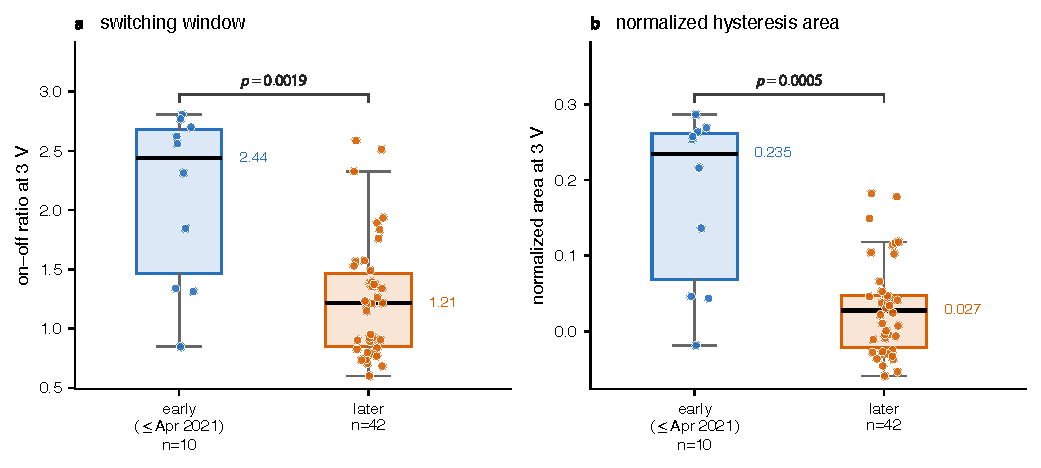
\includegraphics[width=\linewidth]{../figures/chapter3/bridge_window_collapse.pdf}
  \caption[Switching-window collapse at \texorpdfstring{$\sim$}{~}3\,V]{Switching-window collapse across the campaign on the standard \SY{}/\Hybrane{}/\LiTf{}/Ag corpus, read at the $\sim$\SI{3}{\volt} stratum where the window is expressed, one value per device. (a)~On--off ratio and (b)~normalized hysteresis area, both for devices fabricated before the NM\_v026 inflection ($\leq$Apr 2021) versus later. Boxes are quartiles; points are individual devices; the annotated $p$ is a two-sided Mann--Whitney test. The window collapses by roughly a factor of two in on--off ratio and an order of magnitude in area. Reproduced by \texttt{scripts/bridge\_figures.py} (F1).}
  \label{fig:bridge_window}
\end{figure}

\begin{table}[htbp]
  \centering
  \caption[Quantitative degradation signal]{The degradation as a multi-feature signal on the standard corpus, per device. \emph{Window collapse} is read at $\sim$\SI{3}{\volt} as an early-vs-later step at the NM\_v026 inflection (Mann--Whitney). \emph{Ohmic drift} is read at matched $\sim$\SI{1.2}{\volt} as a per-device Spearman correlation with fabrication date, reported with all dates and with the recovery tail ($\geq$2022-03) dropped; the correlation \emph{strengthens} when the reverted batches are removed, as expected if they are partial recoveries. Health flags are shown for completeness and are discussed in the text.}
  \label{tab:bridge_degradation}
  \footnotesize
  \setlength{\tabcolsep}{6pt}
  \renewcommand{\arraystretch}{1.2}
  \resizebox{\linewidth}{!}{%
  \begin{tabular}{l l l l}
    \toprule
    \multicolumn{4}{l}{\textbf{Window collapse @ $\sim$\SI{3}{\volt}} (early $\leq$Apr 2021, $n=10$ vs later, $n=42$)} \\
    \midrule
    Feature & early & later & Mann--Whitney \\
    \midrule
    on--off ratio & \num{2.44} & \num{1.21} & $p=0.0019$ \\
    normalized area & \num{0.235} & \num{0.027} & $p=0.0005$ \\
    \% change in max-V current & $+\SI{17.9}{\percent}$ & $-\SI{2.1}{\percent}$ & $p=0.013$ \\
    \midrule
    \multicolumn{4}{l}{\textbf{Ohmic drift @ matched $\sim$\SI{1.2}{\volt}} (per-device Spearman vs date, $n=64$)} \\
    \midrule
    Feature & all dates & drop recovery tail & \\
    \midrule
    current at max V & $\rho=+0.45$ ($p=0.0002$) & $\rho=+0.55$ ($p<10^{-4}$) & \\
    hysteresis area (V$\cdot\mu$A) & $\rho=+0.57$ ($p<10^{-4}$) & $\rho=+0.69$ ($p<10^{-4}$) & \\
    current difference at on--off & $\rho=+0.51$ ($p<10^{-4}$) & $\rho=+0.63$ ($p<10^{-4}$) & \\
    \midrule
    \multicolumn{4}{l}{\textbf{Health flags} (per-device, $\sim$\SI{1.2}{\volt}, $n=64$)} \\
    \midrule
    \multicolumn{4}{l}{\texttt{is\_broken} \emph{decreases} ($\rho=-0.40$, $p=0.001$) --- a handling metric, \emph{not} degradation;} \\
    \multicolumn{4}{l}{\texttt{is\_saturated} (fails to potentiate) \emph{rises} ($\rho=+0.27$, $p=0.03$).} \\
    \bottomrule
  \end{tabular}%
  }
\end{table}

\paragraph{Mechanism: ohmic drift at matched \boldmath$\sim$\SI{1.2}{\volt}.} The complementary signal lives in the conductivity, read in the tightly matched $\sim$\SI{1.2}{\volt} band so that the sweep-amplitude confound is held fixed. There, the absolute current rises with fabrication date: per device, the current at maximum voltage correlates with date at $\rho=+0.45$ ($p=0.0002$), the raw hysteresis area at $\rho=+0.57$, and the current difference at the on--off point at $\rho=+0.51$ (all $n=64$; \cref{fig:bridge_mechanism}a, \cref{tab:bridge_degradation}). Crucially, these correlations \emph{strengthen} when the deliberately-reverted recovery batches ($\geq$2022-03) are dropped --- to $\rho=+0.55$, $+0.69$, and $+0.63$ respectively --- which is exactly what one expects if those late batches are partial recoveries pulling against the underlying trend. Because the amplitude is held within a narrow band, this is a drift of the material toward more ohmic conduction, not an artefact of the sweep range. The window collapse (relative hysteresis $\to 0$) and the ohmic drift (absolute current $\uparrow$) are two faces of the same degradation. \emph{The magnitudes are deliberately reported as correlations and medians, not as a single multiplicative ``conductivity rise'', because the absolute current depends on the very sweep amplitude being controlled for.}

\begin{figure}[t]
  \centering
  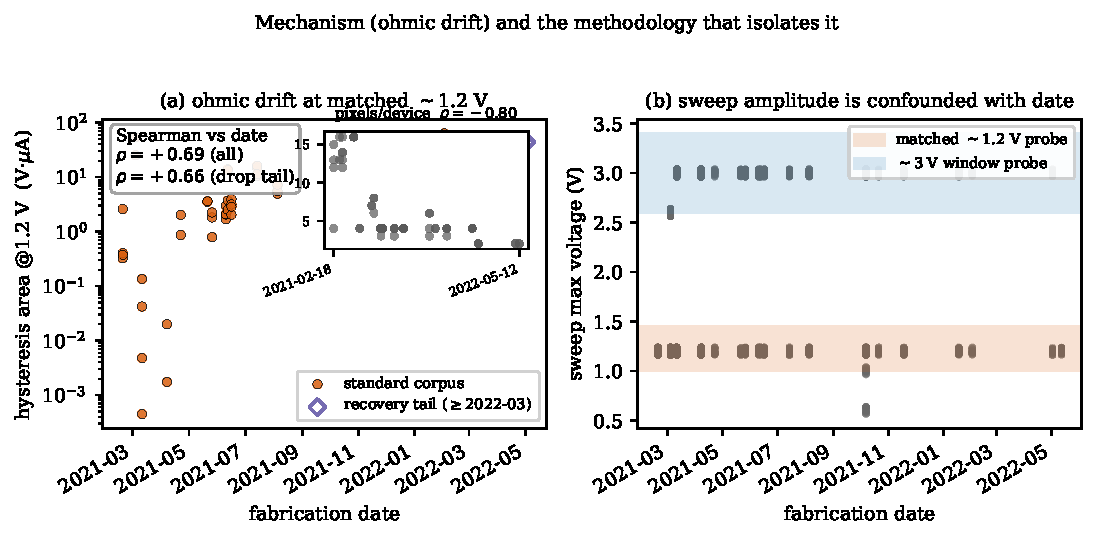
\includegraphics[width=\linewidth]{../figures/chapter3/bridge_mechanism.pdf}
  \caption[Ohmic drift and the methodology that isolates it]{Mechanism and methodology. (a)~Per-device hysteresis area read at the matched $\sim$\SI{1.2}{\volt} band rises with fabrication date (log axis; Spearman $\rho=+0.57$ over all dates, strengthening to $+0.69$ when the recovery-tail batches, open diamonds, $\geq$2022-03, are dropped). \emph{Inset:} the number of pixels measured per device falls over the campaign ($\rho=-0.80$), which is why every statistic is computed per device rather than per pixel. (b)~Sweep amplitude is itself confounded with date: the matched $\sim$\SI{1.2}{\volt} conductivity probe and the $\sim$\SI{3}{\volt} window probe (shaded) are the two strata used throughout, never pooled. Reproduced by \texttt{scripts/bridge\_figures.py} (F2).}
  \label{fig:bridge_mechanism}
\end{figure}

\paragraph{What the health flags do and do not say.} A naive degradation metric would be the fraction of broken devices; it points the wrong way. The curve-level \texttt{is\_broken} flag --- erratic or open-circuit behaviour, a contact and handling failure --- in fact \emph{decreases} over the campaign ($\rho=-0.40$, $p=0.001$), tracking the handling and contacting problems the team progressively fixed (the notes are full of them). It is therefore \emph{not} a degradation metric. The flag that does track the failure is \texttt{is\_saturated} --- a curve whose maximum current fails to exceed the previous one, i.e.\ a device that no longer potentiates --- which rises modestly with date ($\rho=+0.27$, $p=0.03$). The two flags mean different things and are reported separately so that the improvement in handling is not mistaken for the worsening of the device physics.

\subsection{A Candidate Chemistry: Moisture-Driven Hydrolytic Aging of the \Hybrane{} Stock}\label{subsec:bridge_hypothesis}

The rest of this thesis is mechanistic, so a black-box ``the stock went bad'' would be a gap a jury will rightly probe. A definitive answer, however, is \emph{not} supportable from the available record: no electrochemical impedance spectra were ever recorded on any \Hybrane{} device, no gel-permeation chromatography, nuclear-magnetic-resonance or Karl-Fischer analysis was run on the reagent stock, and the aged stock no longer exists in its degraded state. What follows is therefore presented strictly as a hypothesis together with the experiments that would confirm it.

\paragraph{The hypothesis.} \Hybrane{} is a hyperbranched polyester-amide~\cite{Froehling2004,VoitLederer2009}: ester- and amide-rich, and strongly hygroscopic. The leading hypothesis is that, over roughly a year in the bottle, the stock takes up atmospheric water and slowly hydrolyses (chain scission), and that this process could account for the measured electrical signatures without requiring a separate finished-device ageing mechanism.
\begin{itemize}
  \item \textbf{Ohmic drift} (current $\uparrow$ at matched \SI{1.2}{\volt}): absorbed water together with polar scission products raises the baseline ionic and leakage conductivity and plasticises the matrix.
  \item \textbf{Window collapse} (on--off $\to\sim$\num{1.2}, area $\to\sim$\num{0.03}, $\%\Delta I\to-\SI{2}{\percent}$): memristance needs a matrix stiff enough to \emph{hold} a field-displaced ionic profile (the metastable-polarisation picture of \cref{ch:poc}). A plasticised, lower-molecular-weight, water-laden host relaxes and leaks, so the loop closes and successive sweeps stop building up conductance.
  \item \emph{(secondary)} acidic hydrolysis products could partially dope the PPV-type \SY{}, adding a fixed, irreversible conductance --- a second route to the ``high-conductivity, undesirable'' state recorded in the notes.
\end{itemize}

\paragraph{Internal support.} Three lines of evidence already in hand are consistent with the hypothesis, though none closes it. \emph{First}, an annealing-recovery test (\cref{fig:bridge_annealing}): among late, degraded-era devices, aggressive annealing ($\geq$\SI{150}{\celsius}) restores the $\sim$\SI{3}{\volt} window to a median on--off of \num{1.95} ($n=6$) against \num{1.22} for the standard-\SI{75}{\celsius} late devices ($n=44$; Mann--Whitney $p=0.024$, one-sided), back to the early-standard reference level (\num{1.74}). Driving off absorbed water and re-densifying the film is the natural reading; a handling-only or inert-stock story does not predict a thermal recovery. \emph{This test is suggestive, not decisive:} $n=6$ elevated-temperature devices, with co-varying process tweaks, and two of them had measurement-pin issues. \emph{Second}, the full electrical fingerprint --- ohmic drift plus window and potentiation collapse --- is consistent with a water-plasticised, ion-leaky film. \emph{Third}, the material class is, by its very ester and amide linkages, intrinsically susceptible to hydrolytic chain scission, while its polar, hyperbranched architecture is hygroscopic by construction~\cite{Froehling2004,VoitLederer2009}.

\begin{figure}[t]
  \centering
  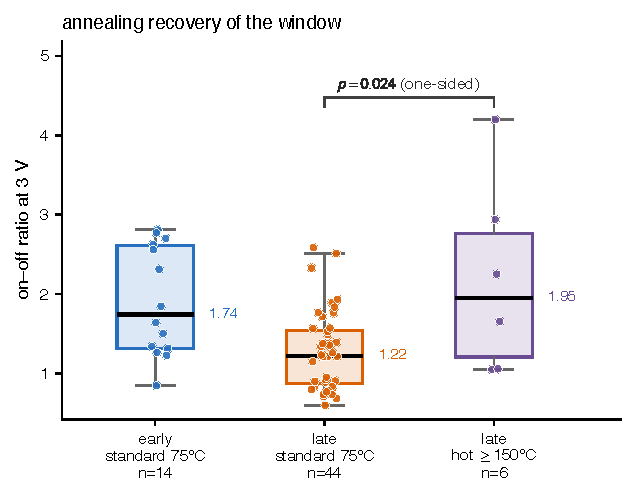
\includegraphics[width=0.62\linewidth]{../figures/chapter3/bridge_annealing_recovery.pdf}
  \caption[Annealing recovery of the switching window]{Annealing-recovery test of the hydrolysis hypothesis (\Hybrane{}/Ag, on--off ratio at $\sim$\SI{3}{\volt}, per device). Among late, degraded-era devices, an aggressive $\geq$\SI{150}{\celsius} anneal restores the window (median \num{1.22}$\to$\num{1.95}) toward the early-standard reference (\num{1.74}); one-sided Mann--Whitney $p=0.024$. Suggestive only ($n=6$ hot devices, co-varying tweaks, two with pin issues). Reproduced by \texttt{scripts/bridge\_figures.py} (F4).}
  \label{fig:bridge_annealing}
\end{figure}

\paragraph{Confirming experiments (future work).} The hypothesis would be tested directly by Fourier-transform infrared spectroscopy (loss of the ester C=O band, growth of --OH) and gel-permeation chromatography (a molecular-weight drop) on \emph{retained aged versus fresh} stock; by Karl-Fischer titration or thermogravimetry for water content; and by impedance spectroscopy to show that the ionic resistance fell. None were run on the \Hybrane{} corpus, so the hypothesis stays open --- and may never fully close, because it concerns a consumable that no longer exists in its aged state.

\FloatBarrier  % flush Table 3.2 (and §3.3 figures) before leaving the section
%% ------------------------------------------------------------
\section{The Resolution: Why PEO}\label{sec:bridge_resolution}
%% ------------------------------------------------------------

The crisis was resolved not by recovering the \Hybrane{} line but by changing the ion-transport host. Replacing the hyperbranched \Hybrane{} with linear poly(ethylene oxide) (\PEO{}) --- the host that carries the comparative study of \cref{ch:comparative} --- delivered two distinct and independently defensible wins. PEO particles are already noted entering the laboratory atmosphere by 2021-12 (NM\_v083), dating the host transition to the height of the investigation.

\paragraph{Win 1 --- a wider, stronger window.} At a matched $\sim$\SI{3}{\volt} sweep, comparing valid (non-broken, non-saturated) devices per device, the \PEO{} host opens a markedly larger switching window than the contemporaneous \Hybrane{} devices: median normalized area \num{0.26} (\Hybrane{}) $\to$ \num{0.42} (\PEO{}), Mann--Whitney $p=0.018$; median on--off ratio \num{2.45} $\to$ \num{4.91} (\cref{fig:bridge_resolution}a,b).

\paragraph{Win 2 --- temporal reproducibility, the actual solution.} This is the crisis solved. Across its full life, the \PEO{}/Ag platform \emph{sustained} a usable switching window over roughly two and a half years (2022--2024, $n=46$ devices): the per-device on--off ratio at $\sim$\SI{3}{\volt} held at a median of \num{2.61}, with yearly medians of \num{3.3}/\num{2.6}/\num{1.9} and no significant downward trend over time. The \Hybrane{} platform, by contrast, sat at a median on--off of \num{1.35} after its stock-driven collapse (\cref{fig:bridge_resolution}c). PEO simply did not exhibit the supply-degradation failure mode --- that absence, sustained over years, is the reproducibility win.

\paragraph{What ``reproducible'' means here.} The claim is precise: it is \emph{temporal / batch} reproducibility --- no stock-driven collapse over years --- and not a claim of superior within-batch, device-to-device uniformity. At matched $\sim$\SI{3}{\volt} the device-to-device coefficients of variation are only modestly different (PEO $\approx$\num{0.38} vs \Hybrane{} $\approx$\num{0.47}), and the chapter does not lean on that gap. The case for \PEO{} rests on the two wins above: a larger window and, above all, the disappearance of the supply-degradation failure over the multi-year span. The attribution of the original failure to the \Hybrane{} host stock (with \SY{} eliminated; \cref{sec:bridge_elimination}) is consistent with this resolution: changing the suspected reagent removed the failure.

\begin{figure}[t]
  \centering
  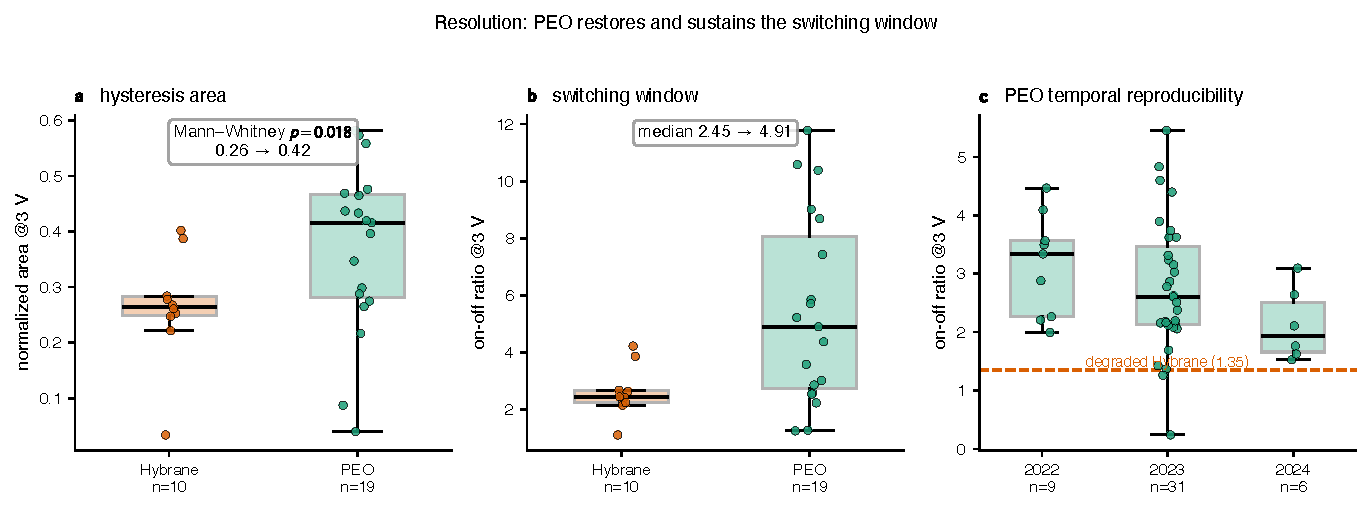
\includegraphics[width=\linewidth]{../figures/chapter3/bridge_resolution.pdf}
  \caption[PEO restores and sustains the switching window]{Resolution of the reproducibility crisis by switching to a \PEO{} host (silver electrode, $\sim$\SI{3}{\volt}, per device). (a)~Normalized hysteresis area and (b)~on--off ratio are larger for \PEO{} than for contemporaneous \Hybrane{} valid devices ($p=0.018$ for area). (c)~PEO temporal reproducibility: the per-device on--off ratio holds at a usable level (median $\approx$\num{2.6}) across 2022--2024 with no collapse, well above the degraded-\Hybrane{} level (dashed line, \num{1.35}). Reproduced by \texttt{scripts/bridge\_figures.py} (F3).}
  \label{fig:bridge_resolution}
\end{figure}

%% ------------------------------------------------------------
\section{Methodological Legacy}\label{sec:bridge_legacy}
%% ------------------------------------------------------------

The diagnosis of the previous sections required instrumentation that did not exist at the start of the campaign. Building it --- provenance capture, a normalized characterization procedure, an automated feature pipeline, and trend-discovery tooling --- is itself a contribution, and, decisively, it is the same instrumentation that produces every quantitative result in the comparative and temporal-computing chapters that follow. The crisis, in other words, paid a lasting dividend. Five durable outputs came out of it.

\begin{itemize}
  \item \textbf{A fabrication-provenance standard.} The per-device library schema (storage atmosphere, illumination, transport, reagent and solvent lots, operator, evaporation profile, and free-text fabrication and characterisation notes) exists \emph{because} the crisis forced the pinning of every variable. It made the elimination of \cref{sec:bridge_elimination} possible and is now the permanent record for every device in the archive.
  \item \textbf{A normalized electrical-characterization procedure.} A hard lesson of \cref{sec:bridge_degradation} is that the protocol sets the response: sweep amplitude alone co-determines the apparent conductivity and whether a window is even expressed. The campaign converged on fixed, documented drive and read protocols so that devices and batches are finally comparable --- the precondition for the comparative chapter.
  \item \textbf{An automated feature pipeline.} The raw instrument traces are reduced to per-device, per-pixel, and per-curve feature tables by a dedicated pipeline; every feature used in this chapter's panel, and in \cref{ch:comparative} and the temporal-computing chapter, is computed there.
  \item \textbf{Trend-discovery and curation tooling.} An interactive feature explorer (with which the present trends were originally found, and whose slicing the four controls of \cref{sec:bridge_degradation} reproduce) and a curation tool that produces the screened device set turn the archive into discoverable trendlines.
  \item \textbf{Figure generation.} A thesis-figure pipeline renders the quantitative figures from the same feature tables, so that every plotted number is traceable to the archive.
\end{itemize}

The framing is forward-looking rather than biographical: the \Hybrane{} failure is, in the end, what made the rest of the thesis measurable. The same apparatus is what the comparative study of \cref{ch:comparative} and the data-driven temporal-computing study build upon.

%% ------------------------------------------------------------
\section{Reconciliation and Bridge}\label{sec:bridge_reconciliation}
%% ------------------------------------------------------------

This chapter must be squared with \cref{ch:poc}, which attributed enhanced shelf stability to the \Hybrane{} matrix. The resolution is a partition, not a retraction, and it turns on the two-metric distinction of \cref{sec:bridge_problem}.
\begin{itemize}
  \item The \emph{published proof-of-concept device} was genuinely stable on the validated $\sim$two-week ambient shelf scale~\cite{PradoSocorro2022}; that claim stands. Indeed, \Hybrane{} \emph{devices} hold their characteristics over weeks to months --- a separate, deliberately long multi-day stability study confirms it, and is reported with the proof-of-concept device --- which is precisely why the failure here is identified as a degradation of the \emph{supply}, not of finished devices.
  \item The \emph{batch-scale reproducibility of the \Hybrane{} platform over the fabrication campaign} is a different metric, and it is the one that collapsed over the following year, in the manner quantified in \cref{sec:bridge_degradation}.
\end{itemize}
The two statements are about different axes (one device over two weeks; the fabrication line over a year) and are both true. The Chapter~\ref*{ch:poc} stability result is therefore preserved intact, and this chapter adds the campaign-scale reproducibility axis that the proof-of-concept study did not probe.

With the reproducibility crisis diagnosed and resolved by the move to a \PEO{} host, the platform is finally in a state where the volatile dynamics can be varied deliberately and compared across many nominally identical devices. That is the task of \cref{ch:comparative}, which treats the \SY{}/\PEO{}/\LiTf{} system on the silver electrode as a replicated composition grid --- using the very provenance standard, normalized protocols, and feature pipeline that this chapter's crisis brought into being --- and asks how the fading-memory dynamics can be engineered through composition and chemistry.

%% ---- Standalone close (skipped when \include'd from thesis.tex) ----
%% A unified bibliography is printed from thesis.tex in the thesis build,
%% so the per-chapter \printbibliography runs only in standalone mode.
\ifdefined\thesismode
  \let\thesisstandaloneclose\relax
\else
  \printbibliography[heading=bibintoc, title={References}]
  \def\thesisstandaloneclose{\end{document}}
\fi
\thesisstandaloneclose

\include{chapters/chapter4_comparative}
%% ============================================================
%%  Chapter 5 — Data-Driven Temporal Computing with
%%              Polymer-Electrolyte Memristor Reservoirs
%%
%%  NOTE: bound as Chapter 5. Internal labels use the ch5_ prefix and
%%  figures live in figures/chapter5/, matching the bound order.
%%
%%  Author : Carlos David Prado-Socorro
%%  Date   : June 2026
%%  Institution : ICMol, Universitat de València
%%
%%  Compile with: latexmk -pdf  (standalone) or via thesis.tex
%%  Plan + evidence: handouts/12_chapter4_demonstration_plan_v4.md,
%%                   handouts/05_chapter4_data_pipeline.md,
%%                   handouts/04_chapter4_temporal_computing_plan.md
%%  Figures: scripts/ch5_figures.py, scripts/ch5_physio_context.py
%% ============================================================

%% ---- Standalone preamble (skipped when \include'd from thesis.tex) ----
\ifdefined\thesismode\else
  \documentclass[12pt, twoside]{report}
  \usepackage{thesis-format}
  \addbibresource{../bibliography/references.bib}
  \begin{document}
  \setcounter{chapter}{4}     % This is Chapter 5 when built standalone
\fi

%% --- Shared macros (\providecommand: harmless if an earlier chapter declared them) ---
\providecommand{\SY}{\textit{Super Yellow}}
\providecommand{\PEO}{PEO}
\providecommand{\LiTf}{LiOTf}
\providecommand{\NaTf}{NaOTf}
\providecommand{\KTf}{KOTf}
\providecommand{\twoterminal}{two-terminal}
\providecommand{\WESAD}{\textsc{wesad}}
\providecommand{\NARMA}{NARMA-10}
%% Standalone-safe reference into this chapter's Supporting Information
%% (Appendix D). Resolves with \cref in the full thesis; prints a literal
%% label in standalone builds, where the appendix is not included.
\providecommand{\siTempRef}[1]{\ifdefined\thesismode\cref{#1}\else Appendix~D\fi}

%% ============================================================
\chapter{Data-Driven Temporal Computing with Polymer-Electrolyte Memristor Reservoirs}\label{ch:temporal}
%% ============================================================

%% ------------------------------------------------------------
\section{Introduction and Scope}\label{sec:ch5_intro}
%% ------------------------------------------------------------

\Cref{ch:poc,ch:comparative} treated the slow, volatile response of these polymer-electrolyte composites first as a phenomenon to be demonstrated and then as a property to be controlled. This chapter treats it as a computational resource. The guiding idea is simple: a device whose conductance carries a fading record of its recent input is, in miniature, a temporal processor, and a collection of such devices is a \emph{reservoir} --- a physical substrate that projects a time-varying input into a high-dimensional state from which simple, linear read-outs can solve temporal tasks.

The chapter rests on a single thesis that connects it to \cref{ch:comparative}: composition and drive \emph{set} the device timescale, and a task \emph{selects} the timescale it needs. The design problem is therefore one of \emph{matching}, and the open question is what a \emph{spread} of timescales --- the low-cost, intrinsic heterogeneity of a solution-processed device family --- buys on top of a single well-chosen one. The destination is a concrete application: low-power, wearable \emph{affective computing} --- the machine recognition of human emotional and physiological state --- whose signals are slow, multi-timescale, and a natural match to these devices. The evidence moves from task-agnostic reservoir benchmarks, to real physiological streams, to \WESAD{} affective classification, and finally to deployment-style tests under sensor noise, consumer wrist-band sensing, and energy and training-cost constraints.

The evidence base is intentionally constrained. Every result is \emph{in silico}: each device node is a compact behavioural model whose parameters are taken directly from the \cref{ch:comparative} fits (\cref{sec:ch5_model}), and every read-out is a single linear regression, so that no claimed computation can be hidden in a nonlinear decoder or a hand-tuned dynamical system. No new devices are fabricated. Two demonstrations run throughout: Demonstration~A asks whether a \emph{single} composition suffices for a single-timescale feature, and Demonstration~B asks what a heterogeneous \emph{bank} adds when the target is multi-timescale. The scoped answer is that the measured device models support temporal-computing demonstrations under constrained read-out conditions, that fading memory is the active ingredient, and that timescale heterogeneity is valuable for memory breadth and task generality but not a guaranteed improvement on every task.

%% ------------------------------------------------------------
\section{Measured Behavioural Model}\label{sec:ch5_model}
%% ------------------------------------------------------------

\Cref{ch:comparative} established that the fading memory of these composites is an engineerable quantity, dominated by composition. To put that memory to work, this chapter reduces each composition cell to a compact behavioural model and treats it as the unit cell of a reservoir computer. The model is deliberately minimal: it is fitted only to the three common measurements of \cref{ch:comparative} --- hysteresis, pulsed potentiation, and delayed depotentiation --- so that every simulation in this chapter traces back to measured data rather than to a hand-tuned dynamical system.

Each composition cell is summarised by a \emph{parameter card}: the write nonlinearity $\phi_c$ from the potentiation curves, the fading-memory law $\lambda_c$ from the depotentiation curves, and an associated device-to-device spread. The fading memory is the stretched-exponential (Kohlrausch) retention identified in \cref{ch:comparative},
\[
  \lambda_c(\Delta t) \;=\; \exp\!\big[-(\Delta t/\tau_c)^{\beta_c}\big],
\]
where $\tau_c$ and $\beta_c$ are the per-cell relaxation time and stretch exponent; for the few cells without an identified stretched fit, a single exponential reproducing the model-free half-life is used instead ($\tau_c = t_{1/2}/\ln 2$, $\beta_c = 1$). The write nonlinearity is the compressive, saturating build-up of conductance with pulse number measured in \cref{ch:comparative}, parametrised by its log--log growth exponent $\alpha_c$ and its peak enhancement.

Driven by a rate-coded input $u_n \in [0,1]$ sampled at interval $\Delta t$, a single device node updates as
\[
  x^{(i)}_n \;=\; \lambda_i\, x^{(i)}_{n-1} \;+\; \big[\max(w_i\, u_n,\,0)\big]^{\alpha_i},
  \qquad \lambda_i = \exp\!\big[-(\Delta t/\tau_i)^{\beta_i}\big],
\]
so that the node integrates a compressive write of its (masked) input and then leaks by exactly the measured retention $\lambda_i$ over the sample interval; $w_i$ is the reservoir input mask. The internal state is read sub-threshold and is therefore assumed state-preserving, as in the proof-of-concept device of \cref{ch:poc}. Every read-out in this chapter is a single \emph{linear} ridge regression on the device states, so that any computation demonstrated is attributable to the devices and not to a nonlinear read-out.

Two constraints are carried explicitly from \cref{ch:comparative} into every result below. First, the write nonlinearity and the fading-memory law were measured at \emph{different write amplitudes} (\SI{3}{\volt} for potentiation, \SI{4}{\volt} for depotentiation; \cref{tab:ch4_protocols}); composing them in a single node is an explicit modelling assumption, not a measured fact, and it most likely under-estimates the true coupling between drive and retention. Second, both were measured at a single, effectively common inter-pulse cadence, so the model is not entitled to claims about input timing finer than that cadence. Both caveats would be removed by the single bench experiment set out in \cref{sec:ch5_limitations}. The per-cell parameter cards inherited from \cref{ch:comparative} and the full set of simulation and read-out settings are tabulated in \siTempRef{app:ch5_settings}.

%% ------------------------------------------------------------
\section{Reservoir Computing and the Common Metric Language}\label{sec:ch5_framework}
%% ------------------------------------------------------------

\paragraph{The reservoir principle.} Reservoir computing emerged from the observation that a fixed, randomly-parametrised dynamical system --- the \emph{reservoir} --- can perform useful temporal computation provided only that a \emph{linear} read-out is trained on its state, leaving the dynamics themselves untrained \cite{Jaeger2001ESN,Maass2002LSM,LukoseviciusJaeger2009}. Two properties make a physical system a useful reservoir candidate: a \emph{fading memory} of past inputs, so that the state reflects recent history but eventually forgets, and a \emph{nonlinear} response, so that the state mixes inputs in ways a linear read-out can exploit. These are precisely the two properties characterised in \cref{ch:comparative} --- the stretched-exponential depotentiation supplies the fading memory, the compressive potentiation supplies the nonlinearity --- which is what makes a bank of these devices a natural candidate substrate for reservoir computing. The same recognition has driven a wave of memristive and organic reservoir demonstrations \cite{Tanaka2019,Du2017,Zhong2021,Cucchi2021}, of which the polymer-electrolyte devices studied here are a low-power, biocompatible instance.

\paragraph{Architecture.} The reservoir used throughout this chapter is a spatial bank of $N$ \emph{independent} device nodes, each a single behavioural model (\cref{sec:ch5_model}) driven by a randomly-masked copy of the input. Independence is a deliberately conservative choice: with no inter-node recurrence, all of the reservoir's richness must come from the spread of intrinsic timescales across compositions, the device-to-device scatter, and the input mask, so any benefit attributed to heterogeneity cannot have been inherited from engineered connectivity. Where a single composition is the subject (Demonstration~A), the same node can equally be deployed as a time-multiplexed, delay-feedback reservoir whose virtual nodes are distributed along a delay line \cite{Appeltant2011}; the two architectures are interchangeable for the present claims, and the spatial bank is used for uniformity.

\paragraph{One ruler.} So that the demonstrations remain comparable, every result is reported on a common set of metrics. The linear \emph{memory capacity} $\mathrm{MC}_k$ and its total \cite{Jaeger2002STM} quantify how much past input is linearly recoverable at each lag, and so visualise timescale coverage directly; \NARMA{} \cite{AtiyaParlos2000} is a standard nonlinear system-identification benchmark; the information-processing-capacity framework \cite{Dambre2012} separates linear from nonlinear contributions and is reported directly in \cref{fig:ch5_ipc}; and the affective tasks are scored by class-balanced macro-F1. Robustness is probed by injecting the measured device-to-device and cycle-to-cycle spread into the bank, reported in \cref{fig:ch5_robustness}.

%% ------------------------------------------------------------
\section{Benchmark Tier: Capacity and System Identification}\label{sec:ch5_benchmarks}
%% ------------------------------------------------------------

The first tier of evidence is deliberately task-agnostic. Two capacity measures --- linear memory capacity and the information-processing capacity that splits it into linear and nonlinear parts --- test reservoir suitability directly, since together they measure the two properties a reservoir must have: fading memory and a usable nonlinearity. A third benchmark, the \NARMA{} system-identification task, is then used not to establish absolute performance but to \emph{rank} the compositions against one another. All three use a random rate-coded input, a bank of $N$ device nodes, and a linear ridge read-out, and all are reported on the same metric ruler so that the two demonstrations of this chapter remain directly comparable.

\paragraph{Memory capacity.} The linear memory capacity of Jaeger measures how much of the past input a reservoir can linearly reconstruct: $\mathrm{MC}_k$ is the squared correlation between a ridge reconstruction of the input $k$ steps ago and its true value, and the total memory capacity is the sum of $\mathrm{MC}_k$ over all lags, bounded above by the number of nodes $N$ \cite{Jaeger2002STM}. \Cref{fig:ch5_mc_curve} compares two banks of equal size ($N=24$): a \emph{homogeneous} bank of jittered copies of the lead cell (\PEO{}~0.3/0.09, differing only by device-to-device scatter) and a \emph{heterogeneous} bank spanning the composition grid ($\tau$ from $\approx 3$ to $\approx 26$\,s). The heterogeneous bank broadens the memory profile across lags and raises the total memory capacity from $4.2$ to $6.4$ (means over ten random input/bank seeds), a factor of $1.54 \pm 0.10$, with near-perfect single-step recall ($\mathrm{MC}_1$ rising from $0.51$ to $1.00$) and the gain concentrated at short-to-intermediate lags. The benefit is positive in all ten seeds and clears a paired test (Wilcoxon signed-rank $p = 0.002$, its floor at this sample size), so the heterogeneity gain is reported with the same statistical discipline as the affective-label null of \cref{sec:ch5_wesad}. Because the nodes are independent --- a bank with no inter-node recurrence --- this is the hard case for a reservoir, and the heterogeneity benefit, which arises purely from the spread of timescales and the device scatter, is therefore a conservative estimate.

\begin{figure}[t]
  \centering
  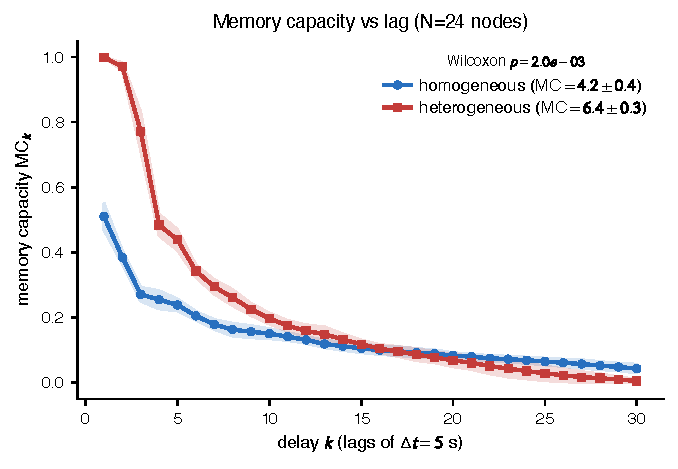
\includegraphics[width=0.66\linewidth]{../figures/chapter5/mc_curve.pdf}
  \caption[Memory capacity versus delay: heterogeneity broadens memory]{Linear memory capacity $\mathrm{MC}_k$ as a function of delay $k$ for a homogeneous bank (all \PEO{} 0.3/0.09 nodes) versus a heterogeneous composition bank ($\tau\approx 3$--$26$\,s). The heterogeneous bank broadens recoverable memory across lags, raising total memory capacity from $4.2$ to $6.4$ (a $1.54\times$ increase; Wilcoxon $p=0.002$ over ten seeds), with the gain concentrated at short-to-intermediate lags. Shaded bands are $\pm 1$\,SD over ten random input/bank seeds. $N=24$ leaky nodes, random uniform input, linear (ridge) read-out; in-silico devices built from the \Cref{ch:comparative} parameter cards.}
  \label{fig:ch5_mc_curve}
\end{figure}

\paragraph{Composition sweep and the single-node optimum.} The same benchmarks, run on single-composition banks, rank the compositions against one another and so test the Demonstration-A claim that one cell suffices for a single-timescale task. \Cref{fig:ch5_composition_sweep} shows that the lead cell \PEO{}~0.3/0.09 attains the highest single-composition memory capacity ($3.98 \pm 0.19$, mean $\pm$ SD over ten seeds), while the neighbouring \PEO{}~0.3/0.045 cell is marginally better on the \NARMA{} system-identification benchmark \cite{AtiyaParlos2000} (NRMSE $0.587 \pm 0.019$ against the lead's $0.616 \pm 0.031$, a close second). Both optima fall in the low-\PEO{} row that \cref{ch:comparative} identifies as carrying the longer fading-memory times, so the benchmark ranking is consistent with the composition result rather than an artefact of the simulation. This supports the Demonstration-A statement: for a single-timescale feature, the lead composition is the memory-capacity optimum and a heterogeneous bank is unnecessary. The \NARMA{} numbers carry only \emph{relative} weight: the absolute error is high ($\approx 0.6$--$0.8$) because a bank of independent, non-recurrent nodes is a weak \NARMA{} reservoir, so the stronger evidence here comes from the capacity measures above (\cref{fig:ch5_mc_curve,fig:ch5_ipc}) and \NARMA{} serves only to corroborate the composition ranking --- a limitation stated rather than hidden, and one a recurrent or delay-feedback architecture would relax.

\begin{figure}[t]
  \centering
  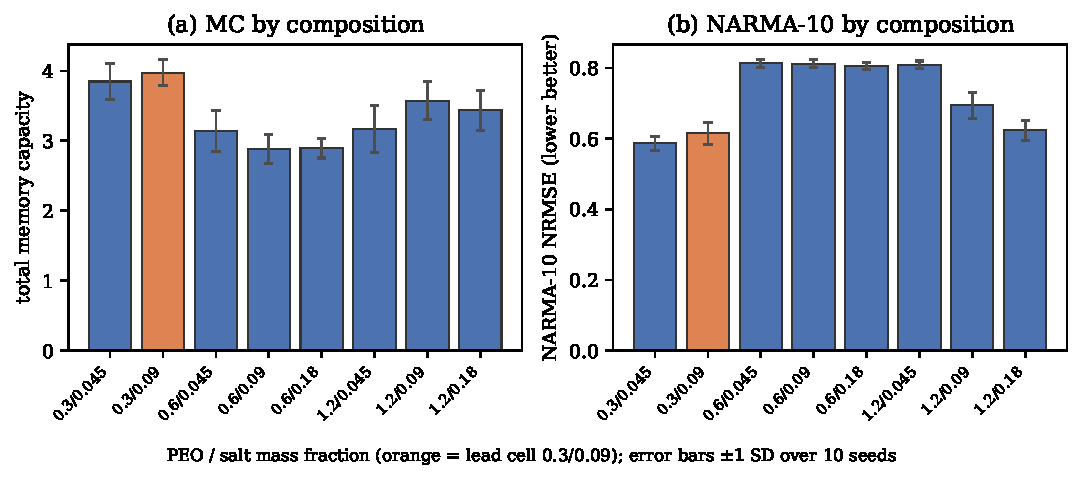
\includegraphics[width=\linewidth]{../figures/chapter5/composition_sweep.pdf}
  \caption[Memory capacity and NARMA across the composition grid]{(a)~Total linear memory capacity and (b)~\NARMA{} reconstruction error (NRMSE, lower is better) for single-composition reservoirs across the \PEO{}/\LiTf{} grid. The lead cell \PEO{}~0.3/0.09 (orange) attains the highest memory capacity; the neighbouring 0.3/0.045 cell is marginally better on \NARMA{}. Both optima fall in the low-\PEO{} row anticipated by \cref{ch:comparative}. Only the \emph{relative} composition ranking is claimed: absolute \NARMA{} NRMSE is high because a bank of independent, non-recurrent leaky nodes is a weak \NARMA{} reservoir.}
  \label{fig:ch5_composition_sweep}
\end{figure}

\paragraph{Linear and nonlinear capacity.} Memory capacity counts only what is \emph{linearly} recoverable. The information-processing-capacity framework of Dambre et al.\ completes the picture by decomposing the total capacity into orthogonal polynomial degrees: degree-one (single-lag) terms give the linear capacity --- essentially the memory capacity --- while degree-two terms (per-lag squares and cross-lag products of the input) give the nonlinear capacity that only a nonlinear reservoir can supply, the whole bounded above by the node count $N$ \cite{Dambre2012}. \Cref{fig:ch5_ipc} reports the split. Even the homogeneous bank carries a substantial nonlinear capacity ($2.7$ of a total $7.1$), which quantitatively supports the interpretation that the compressive potentiation of \cref{ch:comparative} supplies a usable nonlinear response --- the second of the two reservoir prerequisites, alongside fading memory --- rather than merely storing a linear echo. Heterogeneity raises the total capacity from $7.1$ to $11.6$ (paired Wilcoxon $p=0.002$), lifting the linear and nonlinear parts together. The nonlinear capacity is almost entirely degree-two \emph{self} terms (the per-node squaring of the write); cross-lag product terms are negligible, which is the signature of an \emph{independent}, non-recurrent bank that does not multiply inputs across nodes --- consistent with this architecture being, by design, the conservative hard case. That the total sits well below the $N$ bound is likewise expected for leaky nonlinear nodes.

\begin{figure}[t]
  \centering
  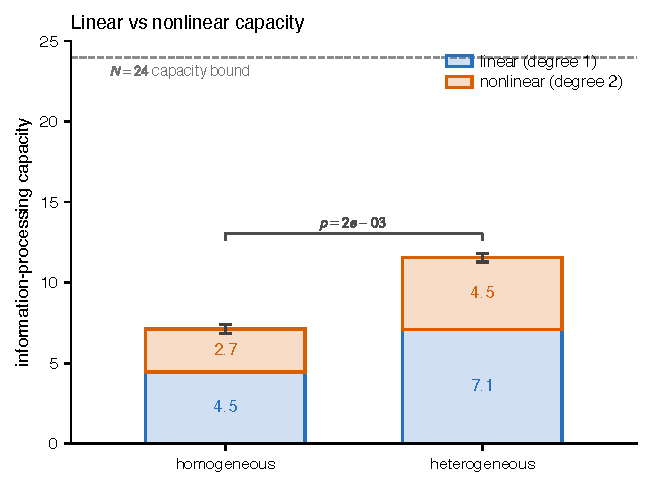
\includegraphics[width=0.52\linewidth]{../figures/chapter5/ipc_capacity.pdf}
  \caption[Information-processing capacity: linear versus nonlinear]{Information-processing capacity \cite{Dambre2012} split into linear (degree-one) and nonlinear (degree-two) parts, for the homogeneous versus the heterogeneous bank ($N=24$, ten seeds). A nonzero nonlinear capacity in both banks indicates that the compressive write supplies a usable nonlinear response, not just linear memory; heterogeneity raises the total from $7.1$ to $11.6$ (paired Wilcoxon $p=0.002$). The dashed line is the $N=24$ upper bound; error bars are $\pm 1$\,SD on the total over seeds.}
  \label{fig:ch5_ipc}
\end{figure}

%% ------------------------------------------------------------
\section{Affective Computing}\label{sec:ch5_affect}
%% ------------------------------------------------------------

Affective computing --- the recognition of human emotional and physiological state by machines --- was framed by Picard as a route to more natural human--computer interaction, classically from \emph{peripheral} physiological signals that are slow, wearable-friendly, and unobtrusive to acquire \cite{Picard1997}. It is the flagship domain of this chapter, for two reasons that follow directly from \cref{ch:comparative}. First, the device timescale window --- fading-memory times from a few seconds to tens of seconds --- sits natively on top of the bands that carry affective information, so no aggressive time-rescaling is needed to bring signal and substrate into register (\cref{tab:ch5_bands}). Second, affective information is \emph{intrinsically multi-timescale}: a fast phasic electrodermal response, a respiration- and heart-rate-variability rhythm of a few seconds, and a tonic level that drifts over minutes all carry state at once~\cite{Boucsein2012EDA,TaskForce1996HRV,ChourpiliadisBhardwaj2022}. That structure is the signal-driven motivation for a heterogeneous bank, and it is also the deployment narrative for an organic, flexible, biocompatible, low-power substrate worn on the skin. \Cref{fig:ch5_tau_coverage} makes the match concrete: it places each composition cell at its measured fading-memory time $\tau$ on the same axis as the affective bands, so that the coverage of the device family --- and, candidly, the one band it does not reach with composition alone --- can be read off directly.

\begin{table}[t]
  \centering
  \small
  \caption[Affective signal timescales and device coverage]{Characteristic timescales of the peripheral affective signals used in this chapter, and the composition cells whose fading-memory window covers them~\cite{Boucsein2012EDA,TaskForce1996HRV,ChourpiliadisBhardwaj2022}. The grid of \cref{ch:comparative} spans the full range, with the lead \PEO{}~0.3 cells serving the slow LF-HRV band.}
  \label{tab:ch5_bands}
  \setlength{\tabcolsep}{5pt}
  \begin{tabular}{lll}
    \toprule
    Affective signal & Timescale & Device coverage \\
    \midrule
    Phasic EDA (SCR) & $\sim$1--10\,s   & low--mid \PEO{} ($t_{1/2}$ 3--19\,s) \\
    Respiration      & $\sim$3--5\,s    & mid \PEO{} \\
    HRV, HF band     & $\sim$2.5--7\,s  & mid \PEO{} \\
    HRV, LF band     & $\sim$7--25\,s   & \PEO{}~0.3 ($\tau \approx 19$--26\,s) \\
    Tonic SCL        & minutes          & slowest / drive-boosted \\
    \bottomrule
  \end{tabular}
\end{table}

\begin{figure}[t]
  \centering
  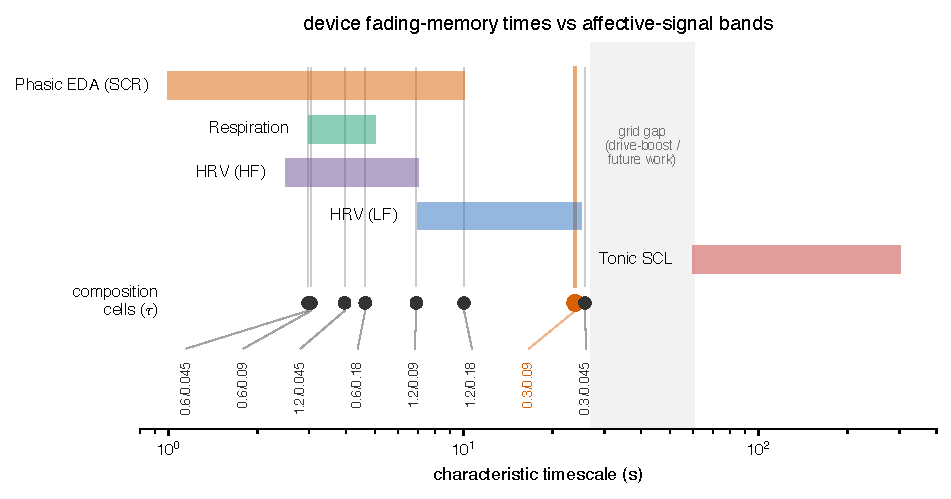
\includegraphics[width=0.82\linewidth]{../figures/chapter5/tau_coverage.pdf}
  \caption[Device timescales versus affective-signal bands]{The \Cref{ch:comparative}-to-\Cref{ch:temporal} bridge as a picture. Each \PEO{}/\LiTf{} composition cell is placed at its measured fading-memory time $\tau$ (markers, lower track) on the same logarithmic time axis as the characteristic timescale bands of the peripheral affective signals (coloured bars; \cref{tab:ch5_bands}). The composition grid ($\tau\approx 3$--$26$\,s) spans the phasic-EDA, respiration and HRV bands, with the lead cell \PEO{}~0.3/0.09 (orange) sitting in the slow LF-HRV band. The tonic, minutes-scale band is not reached by composition alone (shaded gap) and would require the drive-amplitude knob of \cref{ch:comparative} or a slower future cell. This is the visual form of the design rule: an application selects a timescale, and performance follows from how well the device family covers it.}
  \label{fig:ch5_tau_coverage}
\end{figure}

The experiments that follow use the Wearable Stress and Affect Detection corpus (\WESAD{}) of Schmidt et al.\ \cite{Schmidt2018WESAD}: fifteen subjects wearing a chest sensor that records electrodermal activity, respiration, temperature, and an electrocardiogram, with periods labelled baseline, stress, or amusement. \WESAD{} is used in two complementary ways --- as a source of real physiological streams whose multi-lag temporal context the reservoir must encode (\cref{sec:ch5_physio}), and as a downstream affective-classification task (\cref{sec:ch5_wesad}).

%% ------------------------------------------------------------
\section{Physiological Temporal-Context Reconstruction}\label{sec:ch5_physio}
%% ------------------------------------------------------------

The benchmarks of \cref{sec:ch5_benchmarks} prove that a spread of device timescales broadens memory on a \emph{random} input. This section puts that property to a more demanding test on the real, intrinsically multi-timescale affective signals introduced in \cref{sec:ch5_affect}, isolating the multi-timescale \emph{encoding} question before turning to final labels (\cref{sec:ch5_wesad}).

The reservoir is run continuously over each \WESAD{} session at $\Delta t = \SI{1}{\second}$ on four chest channels --- electrodermal activity, respiration, temperature, and an electrocardiogram-derived heart rate --- and a linear read-out reconstructs each channel at delays of $1$, $3$, $8$, $20$ and \SI{45}{\second}. These delays span fast phasic and beat-to-beat context, respiration- and HF-HRV-scale context, and tonic, LF-HRV-scale context~\cite{Boucsein2012EDA,TaskForce1996HRV}. Evaluation is leave-one-subject-out over all fifteen subjects, with $N=48$ nodes per bank.

\Cref{tab:ch5_physio} reports the held-out reconstruction quality. A memoryless bank barely improves on instantaneous input ($R^2 = 0.674$ against $0.673$): with no fading memory, the past is simply not available. Memory of a single timescale lifts $R^2$ to $0.74$, and the heterogeneous composition bank reaches the best single-bank score, $0.756$ --- a gain of $+0.084$ over instantaneous input and $+0.012$ over the best same-size homogeneous control. This last increment is small but unambiguous: scored per subject and paired against the best homogeneous bank across the fifteen subjects, the heterogeneous bank wins in \emph{all fifteen} (Wilcoxon signed-rank $p < 10^{-4}$), so unlike the affective-label increment of \cref{sec:ch5_wesad} it separates cleanly from zero. The mechanism is visible in the band-resolved columns: the fast homogeneous bank is best at the fastest context and the slow homogeneous bank at the slowest, but neither covers the whole vector, whereas the heterogeneous bank is the best \emph{single} bank across the full fast-to-slow physiological context (\cref{fig:ch5_physio}). This is the affect-aligned statement of ``heterogeneity is a computational resource'' on real signals, and it is exactly the result that the final-label classifier of \cref{sec:ch5_wesad} cannot expose.

\begin{table}[t]
  \centering
  \small
  \setlength{\tabcolsep}{5pt}
  \caption[Physiological temporal-context reconstruction on WESAD]{Leave-one-subject-out held-out $R^2$ for multi-lag physiological context reconstruction on \WESAD{} ($N=48$ nodes; means over ten bank seeds where applicable). Bands are reconstruction delays: fast $=1$--$3$\,s, mid $=8$\,s, slow $=20$--$45$\,s. The heterogeneous bank gives the best single-bank score across the full context vector; each homogeneous bank wins only its own band. The heterogeneous advantage over the best homogeneous bank holds in all fifteen subjects (paired Wilcoxon $p<10^{-4}$).}
  \label{tab:ch5_physio}
  \begin{tabular}{lcccc}
    \toprule
    Bank & overall $R^2$ & fast & mid & slow \\
    \midrule
    Instantaneous     & 0.673 & 0.715 & 0.670 & 0.632 \\
    Memoryless        & 0.674 & 0.721 & 0.667 & 0.630 \\
    Homogeneous, fast & 0.741 & \textbf{0.815} & 0.735 & 0.669 \\
    Homogeneous, slow & 0.744 & 0.787 & 0.724 & \textbf{0.711} \\
    Heterogeneous     & \textbf{0.756} & \textbf{0.815} & \textbf{0.737} & 0.708 \\
    \bottomrule
  \end{tabular}
\end{table}

\begin{figure}[t]
  \centering
  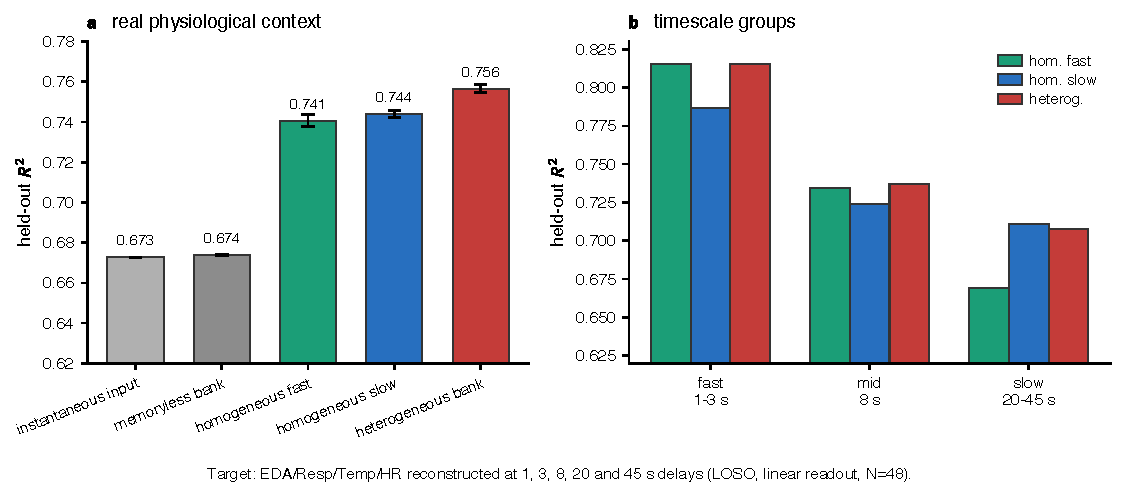
\includegraphics[width=0.82\linewidth]{../figures/chapter5/physio_context_reconstruction.pdf}
  \caption[Physiological temporal-context reconstruction on WESAD]{Multi-lag physiological context reconstruction on real \WESAD{} streams (chest EDA, respiration, temperature, and ECG-derived heart rate). A linear read-out reconstructs each channel at delays of $1$, $3$, $8$, $20$ and $45$\,s from the reservoir state (leave-one-subject-out, $N=48$). The heterogeneous composition bank gives the best single-bank held-out $R^2$ ($0.756$) across the full fast-to-slow context vector, ahead of the best same-size homogeneous control ($0.744$) and well ahead of instantaneous input ($0.673$). Fast and slow homogeneous banks each win only their own band.}
  \label{fig:ch5_physio}
\end{figure}

%% ------------------------------------------------------------
\section{WESAD Affective Classification}\label{sec:ch5_wesad}
%% ------------------------------------------------------------

The downstream task is affective-state classification from the \WESAD{} physiological streams with the device reservoir and a leave-one-subject-out linear read-out. It is reported as a scoped application demonstration: the measured device models support affective classification under the constrained read-out used here, and the contribution of timescale heterogeneity to final labels is reported with error bars, including where it is null. For external calibration, the study that introduced \WESAD{} reports a three-class chest accuracy of $76.5\%$ at macro-F1 $\approx 0.72$ with engineered window features and conventional classifiers under the same leave-one-subject-out protocol, and a binary stress-detection accuracy of $\approx 93\%$ \cite{Schmidt2018WESAD}; the device reservoir's scores below are of the same order. Placed against the wider \WESAD{} literature (\cref{tab:ch5_sota}), which spans engineered-feature classifiers and trained deep networks, the device reservoir's leave-one-subject-out macro-F1 sits in the published performance band, but metric and protocol differences preclude ranking. The comparison shows that a bank of slow organic-memristor models read by a single linear regression can reach a meaningful \WESAD{} performance level under this protocol.

\begin{table}[t]
  \centering
  \small
  \caption[The device reservoir against the WESAD literature]{The device reservoir against representative published \WESAD{} systems. Figures are as reported by each study: classification \emph{accuracy} for the engineered-feature and deep-network systems, the stricter class-balanced \emph{macro-F1} for this work. Metrics and validation protocols differ across studies (Schmidt et al.\ and this work use leave-one-subject-out), so the table is context rather than a head-to-head ranking; its purpose is to show that slow organic-device states with a single linear read-out reach a meaningful WESAD performance level without a trained feature extractor. Binary $=$ stress vs.\ non-stress; three-class $=$ baseline/stress/amusement.}
  \label{tab:ch5_sota}
  \setlength{\tabcolsep}{3pt}
  \begin{tabularx}{\linewidth}{@{}>{\raggedright\arraybackslash}p{2.7cm}>{\raggedright\arraybackslash}Xcc@{}}
    \toprule
    Study & Approach & Three-class & Binary \\
    \midrule
    Schmidt et al.\ (2018)~\cite{Schmidt2018WESAD}   & engineered features, AdaBoost/RF & $76.5\%$ (F1 $0.72$) & $93.0\%$ \\
    Bobade \& Vani (2020)~\cite{Bobade2020}          & engineered features, neural net  & $84.3\%$ & $95.2\%$ \\
    Gil-Mart{\'\i}n et al.\ (2022)~\cite{GilMartin2022} & CNN on spectral features      & $85.1\%$ & $96.6\%$ \\
    \textbf{This work} & device-reservoir states, linear read-out & F1 $0.758$ & F1 $0.894$ \\
    \bottomrule
  \end{tabularx}
\end{table}

\paragraph{Demonstration~A: a single composition suffices for a single-timescale feature.} Binary stress-versus-baseline classification from electrodermal activity, read out at the window level from the lead composition alone, reaches a leave-one-subject-out macro-F1 of $0.894$ (\cref{fig:ch5_wesad}a). This supports the Demonstration-A claim that one well-matched composition can act as a useful affect-aligned node. It comes, however, with an instructive caveat: a static feature baseline (the mean, standard deviation, last value and slope of the same signal) matches it ($0.899$). The 60-second-window task is therefore quasi-static --- the discriminative information sits in the instantaneous signal level, not in its temporal history --- which is exactly why timescale heterogeneity has nothing to contribute here, and why a memory-demanding reformulation is needed to test the heterogeneity claim fairly.

\paragraph{Demonstration~B: streaming three-class tracking.} The fair test is a streaming one: the reservoir runs continuously over each session and the affective class (baseline, stress, or amusement) is read out at \emph{every} step, so that the task is designed to use fading memory rather than a static window summary. \Cref{tab:ch5_wesad} decomposes the result into four matched-size banks. Relative to instantaneous input, adding dimensionality (a same-size memoryless bank) contributes $+0.028$, adding fading memory of a single timescale a further $+0.016$, and adding timescale heterogeneity a final $+0.005$. The measured fading-memory gain over a same-size memoryless bank is a modest but consistent $+0.014$ to $+0.020$. The timescale-heterogeneity increment, however, is $+0.005 \pm 0.011$ --- within seed noise (positive in seven of ten seeds; across sampling intervals from $0.5$ to \SI{4}{\second} the heterogeneous-minus-homogeneous gap stays in $[+0.002,+0.007]$ but never separates from zero). Per class, the best bank reaches F1 $0.90$ on baseline and $0.92$ on stress but only $0.55$ on the amusement class, which is the hard class for every model. The reason is an elicitation limit, not a memory-horizon one: amusement is the shortest \WESAD{} condition (roughly $5.6$\,ks of labelled data against $17.6$\,ks of baseline and $10.0$\,ks of stress) and the lowest in autonomic arousal, so its physiological signature is both weak and under-represented. Consistently, no bank from memoryless to heterogeneous recovers it, which is why the class limits every model rather than discriminating between them.

\begin{table}[t]
  \centering
  \small
  \caption[Streaming three-class affect tracking on WESAD]{Leave-one-subject-out macro-F1 for streaming three-class \WESAD{} tracking (means $\pm$ SD over ten bank seeds; matched input masks). Each increment is the gain over the row above: fading memory contributes a small, consistent gain, while the timescale-heterogeneity increment is within noise (\textit{ns}).}
  \label{tab:ch5_wesad}
  \begin{tabular}{lcc}
    \toprule
    Bank & macro-F1 & increment \\
    \midrule
    Instantaneous (no memory)             & 0.709             & --- \\
    Memoryless (dimensionality only)      & 0.737             & $+0.028$ \\
    Homogeneous (memory, single $\tau$)   & $0.753 \pm 0.009$ & $+0.016$ \\
    Heterogeneous (memory, $\tau$ spread) & $0.758 \pm 0.006$ & $+0.005$ (\textit{ns}) \\
    \bottomrule
  \end{tabular}
\end{table}

\begin{figure}[t]
  \centering
  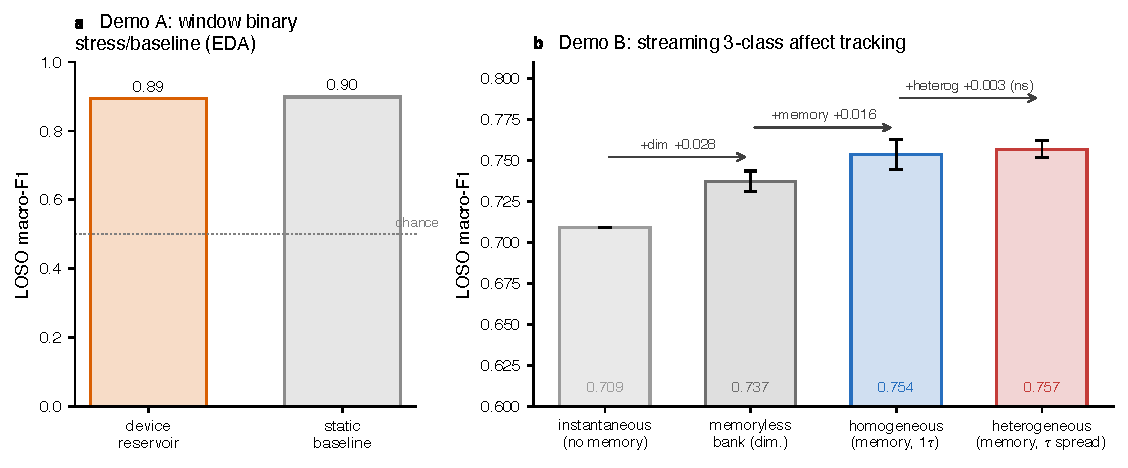
\includegraphics[width=\linewidth]{../figures/chapter5/wesad_affect.pdf}
  \caption[WESAD affective classification with device reservoirs]{Affective classification with in-silico device reservoirs (leave-one-subject-out, linear read-out). (a)~Demonstration A, window-level binary stress-versus-baseline from EDA: the single lead composition matches a static feature baseline, i.e.\ the $60$\,s-window task is quasi-static and requires no fading memory. (b)~Demonstration B, streaming three-class affect tracking (baseline/stress/amusement) decomposed as instantaneous $\rightarrow$ $+$dimensionality $\rightarrow$ $+$fading memory $\rightarrow$ $+$timescale heterogeneity. Fading memory contributes a small but consistent gain; the timescale-heterogeneity increment ($+0.005\pm0.011$) is within seed noise. Error bars are $\pm 1$\,SD over $10$ bank seeds.}
  \label{fig:ch5_wesad}
\end{figure}

\paragraph{Why heterogeneity does not pay off on the labels.} The null is not a failure of the devices but a property of the task. Affect labels are slowly varying, sustained states; their discriminative memory demand is dominated by a single slow, tonic band that the lead composition's relaxation time ($\tau \approx 19$--$26$\,s) already serves. Timescale heterogeneity converts into task performance only when the target requires memory at many distinct lags \emph{simultaneously} --- which the memory-capacity benchmark (\cref{fig:ch5_mc_curve}) and the physiological-context reconstruction (\cref{tab:ch5_physio}) both demand, and on which heterogeneity does pay, but which a single sustained label set does not. The reading carried into \cref{sec:ch5_designrules} is that the measured device models support affective classification under this protocol, that fading memory helps, and that composition-timescale \emph{matching} is the operative design lever --- with heterogeneity a generality and robustness hedge rather than a guaranteed win on any one label set.

%% ------------------------------------------------------------
\section{Continuous Monitoring Under Deployment Conditions}\label{sec:ch5_robust}
%% ------------------------------------------------------------

The scores of \cref{sec:ch5_wesad} are dominated by long stretches of sustained state, where the instantaneous signal level already carries the label --- which is precisely why a static feature baseline ties the reservoir on the quasi-static window task. A wearable in the field is judged on what those averages hide. It must keep working while the wearer moves and the sensor is noisy, and motion artefact is the dominant failure mode of wrist-worn electrodermal and photoplethysmographic sensing. This is a temporal problem on which fading memory has a structural advantage: a leaky integrator is a temporal low-pass that averages transient artefact away, whereas an instantaneous read reacts to every spike.

\Cref{fig:ch5_robust_monitoring} makes the point on a continuous binary stress detector --- stress versus baseline-plus-amusement, read out at every step, leave-one-subject-out, with the same single linear read-out used throughout. On clean streams every bank is competitive (macro-F1 $\approx 0.91$--$0.92$, of the order of the $\approx 93\%$ binary benchmark of the corpus~\cite{Schmidt2018WESAD}), the static read among them, exactly as the window task warned. As progressively stronger sensor noise and motion-artefact bursts are injected, the instantaneous and memoryless controls degrade steeply --- macro-F1 from $0.914$ to $0.840$ by an injected noise of $\sigma = 0.4$ of the signal range --- while the fading-memory banks barely move, holding $\approx 0.92$ across the whole range. At $\sigma = 0.4$ the advantage of the heterogeneous memory bank over the instantaneous read is $+0.088$, positive in all fifteen subjects (paired Wilcoxon $p < 10^{-4}$); and even on clean streams, fading memory roughly halves the false-alarm rate ($0.046 \to 0.026$), the spurious-alert cost that most limits a deployed affect monitor. The active ingredient is memory itself, not its spread: the homogeneous and heterogeneous banks are equally robust, consistent with the design rule below. Two boundaries are reported with the result rather than around it: the accuracy gain in the narrow window straddling label transitions is positive ($0.747 \to 0.775$) but not resolved across subjects, and the detection latency is comparable across banks, set by the prediction-smoothing horizon rather than by the device. The deployment-relevant statement is therefore specifically about robustness --- under the corruption a real wearable faces, the temporal device sustains a stress detector that the static baseline, competitive only in laboratory-clean conditions, does not.

\begin{figure}[t]
  \centering
  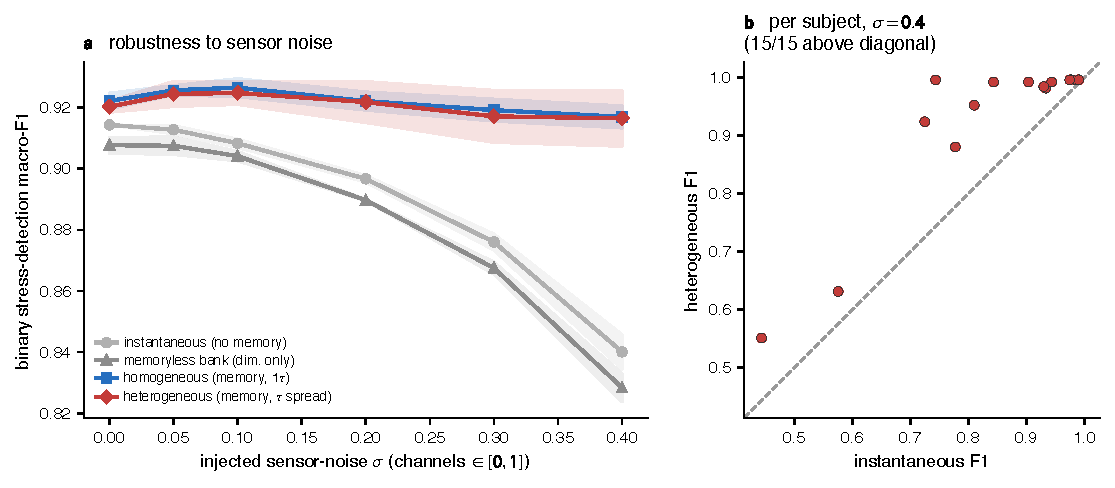
\includegraphics[width=\linewidth]{../figures/chapter5/robust_monitoring.pdf}
  \caption[Continuous stress monitoring is robust to sensor noise]{Continuous stress monitoring with device reservoirs (binary stress vs.\ baseline-plus-amusement, per-step, leave-one-subject-out, linear read-out). (a)~Detection macro-F1 against the magnitude $\sigma$ of injected sensor noise and motion-artefact bursts: the fading-memory banks (homogeneous, heterogeneous) stay flat at $\approx 0.92$, while the instantaneous and memoryless controls collapse, because temporal integration rejects transient artefact. Bands are $\pm 1$\,SD over seeds. (b)~Per-subject scores at $\sigma=0.4$: the heterogeneous memory bank beats the instantaneous read in all fifteen subjects (paired Wilcoxon $p<10^{-4}$). Memory, not its heterogeneity, is the active ingredient; the homogeneous bank is equally robust.}
  \label{fig:ch5_robust_monitoring}
\end{figure}

\paragraph{Cross-corpus replication.} A single corpus cannot establish generality, so the robustness test was repeated on an independent dataset: the PhysioNet Non-EEG corpus of Birjandtalab et al.~\cite{Birjandtalab2016}, twenty subjects wearing a \emph{different} wrist sensor (an Affectiva Q recording electrodermal activity and skin temperature, with a pulse-oximeter heart rate) through relaxation and cognitive, emotional, and physical stress phases. Taking cognitive and emotional stress as the stress class against relaxation --- the psychosocial analogue of the \WESAD{} stressor, with the physical-exertion phase held out as a different mechanism whose racing heart rate is trivially separable from the instantaneous signal alone --- and running the identical detector reproduces the \WESAD{} result on this independent sensor and population (\cref{tab:ch5_crosscorpus}). The corpus is harder in absolute terms (clean macro-F1 $\approx 0.65$--$0.68$, against $\approx 0.91$ on the cleaner \WESAD{} chest signals) and, as on \WESAD{}, the clean-stream memory advantage is small and not resolved. But under sensor noise the same divergence reappears, more sharply: the instantaneous detector falls from $0.651$ to $0.516$ while the fading-memory bank holds near $0.66$, a $+0.130$ advantage at $\sigma=0.4$ that is positive in nineteen of the twenty subjects (paired Wilcoxon $p<10^{-5}$). The noise-robustness of the temporal substrate is therefore not a property of one dataset; it transfers to a new corpus, sensor, and population.

\begin{table}[t]
  \centering
  \small
  \caption[Cross-corpus replication on the PhysioNet Non-EEG dataset]{Cross-corpus replication of the noise-robustness result on the independent PhysioNet Non-EEG stress corpus~\cite{Birjandtalab2016} (twenty subjects; Affectiva Q wrist electrodermal activity and temperature plus pulse-oximeter heart rate; cognitive and emotional stress versus relaxation; leave-one-subject-out, linear read-out). As on \WESAD{}, the instantaneous detector collapses under injected sensor noise while the fading-memory banks hold; the heterogeneous-minus-instantaneous advantage at $\sigma=0.4$ is $+0.130$ ($19/20$ subjects, $p<10^{-5}$). Memory, not its spread, is again the active ingredient.}
  \label{tab:ch5_crosscorpus}
  \setlength{\tabcolsep}{8pt}
  \begin{tabular}{lcc}
    \toprule
    Detector & macro-F1 (clean) & macro-F1 ($\sigma=0.4$) \\
    \midrule
    Instantaneous (no memory) & 0.651 & 0.516 \\
    Homogeneous (memory)      & \textbf{0.682} & \textbf{0.657} \\
    Heterogeneous (memory)    & 0.667 & 0.646 \\
    \bottomrule
  \end{tabular}
\end{table}

%% ------------------------------------------------------------
\section{Toward a Worn Device: Sensor Site and Operating Budget}\label{sec:ch5_deploy}
%% ------------------------------------------------------------

The robustness of the previous section is a laboratory statement until two further questions are answered: whether the advantage survives a consumer-grade sensor, and what the device would cost to run. Both are answered from the same measured ingredients --- the \WESAD{} wrist recordings and the device constants of \cref{ch:poc} --- without any new assumption.

\paragraph{Sensor site.} \WESAD{} records every session twice: from a chest strap (the clean electrocardiogram and respiration used so far) and from an Empatica E4 wrist band, the form factor of a real affective wearable but with fewer and far noisier channels --- skin conductance, skin temperature, and a photoplethysmogram from which heart rate must be recovered, with no respiration. Re-running the continuous stress detector of \cref{sec:ch5_robust} on the wrist signals (\cref{tab:ch5_wrist}) tells a consistent story. The static, instantaneous detector loses ground on the wrist, its clean macro-F1 falling from $0.914$ on the chest to $0.881$ as the noisier photoplethysmographic heart rate and the missing respiration channel degrade the instantaneous signal. The fading-memory reservoir is essentially unaffected by the move to the wrist ($0.920 \to 0.922$): it recovers from temporal context what the static read loses to channel quality. The memory advantage is therefore much larger on the consumer wrist than on the chest ($+0.041$ on clean streams against $+0.006$, and a sustained $+0.069$ under injected noise), which is the right way round for deployment --- the harder, more realistic sensor is exactly where the temporal substrate helps most, and fading memory cuts the wrist false-alarm rate by about a third ($0.062 \to 0.040$).

\begin{table}[t]
  \centering
  \small
  \caption[Stress detection: chest versus consumer wrist sensor]{Continuous binary stress-detection macro-F1 on the \WESAD{} chest strap versus the Empatica E4 wrist band (leave-one-subject-out, linear read-out). Moving to the noisier consumer sensor degrades the instantaneous (static) detector but not the fading-memory reservoir, so the memory advantage is larger on the wrist; $\sigma$ is the injected sensor-noise level of \cref{fig:ch5_robust_monitoring}.}
  \label{tab:ch5_wrist}
  \setlength{\tabcolsep}{5pt}
  \begin{tabularx}{\linewidth}{@{}>{\raggedright\arraybackslash}Xcccc@{}}
    \toprule
    & \multicolumn{2}{c}{Chest} & \multicolumn{2}{c}{Wrist E4} \\
    \cmidrule(lr){2-3}\cmidrule(lr){4-5}
    Detector & clean & $\sigma=0.4$ & clean & $\sigma=0.4$ \\
    \midrule
    Instantaneous (no memory)   & 0.914 & 0.840 & 0.881 & 0.847 \\
    Memory reservoir (het)      & \textbf{0.920} & \textbf{0.916} & \textbf{0.922} & \textbf{0.916} \\
    \bottomrule
  \end{tabularx}
\end{table}

\paragraph{Operating budget.} The reservoir's appeal for a worn device is that temporal filtering is delegated to the material dynamics: the dynamics are fixed and untrained, and only the linear read-out is fitted, by a single closed-form ridge solve rather than gradient descent. The trained part is therefore one $(N{+}1)\times K$ weight matrix --- $75$ weights for the $N=24$, three-class banks here, $147$ for the $N=48$ banks --- against the $10^{4}$ to $10^{6}$ trainable weights of the deep models usually brought to wearable affect, a reduction of roughly two to four orders of magnitude that puts on-device, per-user calibration within reach. The energy budget follows from the measured device of \cref{ch:poc}: at the proof-of-concept energy of $\approx\SI{50}{\nano\joule}$ per write event ($\approx\SI{6}{\femto\joule\per\micro\metre\squared}$ over the \SI{0.0825}{\square\centi\metre} junction), charging each of $N$ nodes once per one-second update draws of order a microwatt ($\approx\SI{1.2}{\micro\watt}$ at $N=24$), while the read-out is $N\,K$ multiply--accumulates, well under a nanojoule per step. These are unoptimised, large-area figures; reducing the junction toward the integrated-device regime would cut the per-event energy by orders of magnitude. The point is the order of magnitude and the contrast in kind: the device responds in the sub-kilohertz regime, comfortably above the sub-hertz bandwidth of affective physiology, so the substrate is never the bottleneck, and the temporal feature extraction that a digital pipeline would compute explicitly is performed by the device dynamics during the write/read cycle. The full budget and its assumptions are tabulated in \siTempRef{app:ch5_deploy}.

%% ------------------------------------------------------------
\section{Design Rule: Match Timescale to Task}\label{sec:ch5_designrules}
%% ------------------------------------------------------------

\Cref{sec:ch5_benchmarks,sec:ch5_physio,sec:ch5_wesad} complete the design rule opened in \cref{ch:comparative}. Composition and drive \emph{set} the fading-memory timescale; an application \emph{selects} one timescale, or a set of timescales, and performance follows from how well the device family covers them (\cref{fig:ch5_tau_coverage}). The composition sweep gives the single-timescale case (\cref{fig:ch5_composition_sweep}): the lead cell is the memory-capacity optimum because its relaxation time best matches a seconds-scale target. The multi-lag physiological task gives the opposite case (\cref{tab:ch5_physio}): when the target spans bands that no single cell covers, the bank whose timescales are \emph{spread} to match them is the best single choice.

\paragraph{Memory first, heterogeneity as a generality hedge.} The results give a consistent account of what these resources are worth, drawn together in \cref{tab:ch5_summary}. The first-order effect is \emph{fading memory itself}: every memory bank, homogeneous or heterogeneous, far exceeds the memoryless and instantaneous baselines, and the gap widens to as much as $+0.08$ macro-F1 under the sensor noise of a worn device (\cref{sec:ch5_robust,sec:ch5_deploy}). The second-order effect is the \emph{spread} of timescales. Where the task demands memory at many lags at once --- random-input memory capacity (a $1.54\times$ broadening, $p=0.002$; \cref{fig:ch5_mc_curve}) and real-physiology context reconstruction ($+0.012$ in held-out $R^2$ over the best homogeneous bank, $15/15$ subjects, $p<10^{-4}$; \cref{tab:ch5_physio}) --- heterogeneity is a measurable, statistically resolved resource. Where a single slow timescale already dominates, as in the sustained stress labels and the single-channel monitoring task, the best-matched single composition is as good or marginally better, exactly as Demonstration~A anticipated. The two readings combine into a deployment rule: because a heterogeneous bank gives up at most about a hundredth of a point on the single-timescale tasks but gains substantially on the multi-timescale ones, it is the rational default for a substrate fabricated once and reused across an unknown mix of affective tasks. Crucially for the materials argument of this thesis, that heterogeneity is \emph{low-cost and intrinsic}: it arises naturally in a solution-processed device family through composition spread, device-to-device scatter, and --- as further, illustrative knobs catalogued in \cref{ch:comparative} but not required by the quantitative banks here --- electrolyte chemistry and drive amplitude.

\begin{table}[t]
  \centering
  \small
  \caption[Fading memory versus its spread across the affective workload]{Fading memory versus its spread across the affective workload of this chapter. Every memory bank (homogeneous, heterogeneous) far exceeds the memoryless instantaneous baseline --- decisively so under the sensor noise of a worn device --- so fading memory is the first-order resource. The heterogeneous bank then wins where several timescales matter at once (physiological context), while the best-matched single composition wins where one timescale dominates (sustained labels, single-channel monitoring); the gap between them never exceeds about $0.01$ macro-F1. Bold marks the best bank per row. Scores from \cref{tab:ch5_physio,tab:ch5_wesad} and \cref{sec:ch5_robust,sec:ch5_deploy}.}
  \label{tab:ch5_summary}
  \setlength{\tabcolsep}{4pt}
  \begin{tabularx}{\linewidth}{@{}>{\raggedright\arraybackslash}Xlccc@{}}
    \toprule
    Affective task & Metric & Instantaneous & Homogeneous & Heterogeneous \\
    \midrule
    Physiological context (multi-$\tau$) & $R^2$       & 0.673 & 0.744 & \textbf{0.756} \\
    Three-class affect tracking          & macro-F1    & 0.709 & 0.753 & \textbf{0.758} \\
    Stress monitoring, clean             & macro-F1    & 0.914 & \textbf{0.922} & 0.920 \\
    Stress monitoring, $\sigma{=}0.4$    & macro-F1    & 0.840 & \textbf{0.917} & 0.916 \\
    Wrist stress, clean                  & macro-F1    & 0.881 & \textbf{0.930} & 0.922 \\
    Wrist stress, $\sigma{=}0.4$         & macro-F1    & 0.847 & \textbf{0.918} & 0.916 \\
    \bottomrule
  \end{tabularx}
\end{table}

\paragraph{Operating point and integration.} The same parameter cards that drive the simulations also fix the deployment envelope. The devices operate in the sub-kilohertz regime in which affective physiology lives, so the slow response that disqualifies them for fast logic is exactly what suits them to on-skin sensing. The read-out is assumed sub-threshold and state-preserving, which sets a read-voltage and read-disturb budget that any circuit implementation must respect; and the device-to-device scatter that a memory application would treat as a yield problem is, in the reservoir setting, part of the computational substrate. \Cref{fig:ch5_robustness} makes this last point quantitative and is perhaps the clearest single statement of the reservoir's tolerance to the imperfection of solution processing: total memory capacity is reported against the magnitude of injected device-to-device scatter, and the heterogeneous bank holds its advantage across the whole realistic range --- including at the \emph{measured} scatter, \(\sigma(\ln\tau)\approx\num{0.85}\), estimated from the silver \PEO{}/\LiTf{} devices within each fixed composition cell and confirmed to be unexplained by spin speed, anneal, film thickness, or device age (\siTempRef{app:ch5_scatter}). The limiting case is instructive --- a bank of \emph{identical} nodes (zero scatter) is nearly memory-less, because perfectly matched nodes are redundant, so the scatter that yield engineering fights to remove is precisely what a homogeneous reservoir lives on, while the heterogeneous bank additionally carries intrinsic timescale spread and therefore degrades most gracefully. These are the design rules that \cref{ch:comparative} makes available and that an eventual hardware reservoir would inherit.

\begin{figure}[t]
  \centering
  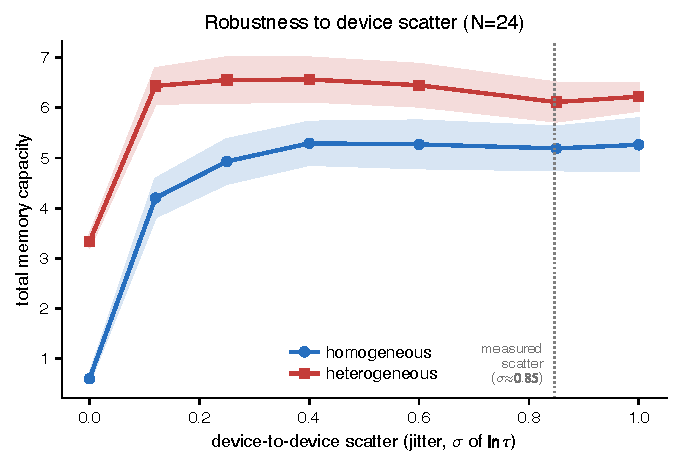
\includegraphics[width=0.6\linewidth]{../figures/chapter5/robustness.pdf}
  \caption[Robustness to device-to-device scatter]{Total memory capacity versus the magnitude of injected device-to-device scatter (jitter on $\tau$, $\beta$ and $\alpha$), for the homogeneous and heterogeneous banks ($N=24$, ten seeds; shaded bands $\pm 1$\,SD). The heterogeneous bank keeps its advantage across the entire realistic spread, including at the measured device-to-device scatter (dotted line: \(\sigma(\ln\tau)\approx\num{0.85}\), derived in \siTempRef{app:ch5_scatter}). A bank of perfectly identical nodes (zero scatter) is nearly memory-less because matched nodes are redundant: the scatter that yield engineering fights to remove is what the reservoir computes on.}
  \label{fig:ch5_robustness}
\end{figure}

%% ------------------------------------------------------------
\section{Limitations and Scope Conditions}\label{sec:ch5_limitations}
%% ------------------------------------------------------------

The claims of this chapter are bounded by scope conditions that are stated here in full, in keeping with the claim discipline of \cref{ch:comparative}.

\paragraph{In silico.} The demonstrations are simulations. Each node is the measured $\phi \otimes \lambda \otimes f$ behavioural model of \cref{sec:ch5_model}, not a bench reservoir, and every figure caption names the data behind it; the step from a fitted per-device model to a wired hardware reservoir is left to future work.

\paragraph{The composition assumption.} As detailed in \cref{sec:ch5_model}, the write nonlinearity and the fading-memory law were measured separately, at different write amplitudes and a single inter-pulse cadence. Composing them assumes the two regimes are compatible and probably under-estimates the coupling between drive and retention. A single matched-amplitude experiment that sweeps pulse count and inter-pulse interval together would remove the assumption; it is the most important bench experiment this chapter calls for.

\paragraph{Operating regime and read-out.} The model is identified, and valid, only in the slow, sub-kilohertz regime of the measurements; affective signals fall natively in this band, but fast temporal tasks are out of scope. Every read-out is a single ridge regression --- a deliberate constraint, since a nonlinear read-out could solve the tasks by itself and would invalidate the reservoir claim --- and the read is assumed sub-threshold and state-preserving.

\paragraph{Heterogeneity axes.} The quantitative heterogeneous banks span the replicated \PEO{}/\LiTf{} composition grid. The chemistry and drive-amplitude axes of \cref{ch:comparative}, being sample-limited ($n\le 2$ per matched cell), enter only as illustrative additional knobs; Demonstration~B is therefore a principle demonstration of composition heterogeneity, not a powered comparison across chemistries. The composition cells that define these banks index \emph{composition}, not film thickness: although spin-coating speed and residual film thickness covary with the \PEO{} fraction, the parameter cards inherited here were shown to be governed by composition rather than thickness (\cref{fig:ch4_thickness_control}, \cref{sec:ch4_materials}), so the heterogeneity exploited in this chapter is compositional in origin.

\paragraph{Corpora, and a reported null.} The affective classification results rest principally on one corpus (\WESAD{}); the deployment-critical noise-robustness finding is replicated on a second, independent corpus, wrist sensor, and population (the PhysioNet Non-EEG dataset, \cref{sec:ch5_robust}), but a broader multi-corpus study, and the affective dimensions beyond stress such as continuous valence and arousal, remain future work. The central negative result --- that timescale heterogeneity does not separably improve final-label classification --- is reported with error bars across seeds and sampling intervals rather than omitted, because it is informative: it localises exactly where heterogeneity helps and where it does not.

%% ------------------------------------------------------------
\section{Summary and Bridge to the Conclusions}\label{sec:ch5_conclusions}
%% ------------------------------------------------------------

This chapter has shown that compact behavioural models of solution-processed polymer-electrolyte memristors, characterised through the three common measurements of \cref{ch:comparative} and read out by a single linear regression, can support temporal-computing demonstrations within the stated in-silico scope. The models produce a resolved memory-capacity gain for heterogeneous banks, give a relative \NARMA{} composition ranking, encode the multi-lag temporal context of real physiological signals, and classify affective state from the \WESAD{} corpus at a leave-one-subject-out macro-F1 of $0.894$ on a binary stress task and $0.758$ on a three-class streaming task. Beyond accuracy on curated splits, the same models sustain a continuous stress detector under the sensor noise and on the consumer wrist band that a worn device must tolerate --- where fading memory holds detection near $0.92$ macro-F1 while a static baseline collapses to $0.84$ ($+0.088$, all fifteen subjects, $p<10^{-4}$) --- at an estimated always-on budget of order a microwatt and only the tens-to-a-hundred trained read-out weights of one ridge solve, against the $10^4$--$10^6$ gradient-trained weights of a deep model of comparable accuracy.

The results resolve into a single design rule that unifies the two experimental chapters. \Cref{ch:comparative} establishes that composition and drive set the device timescale; this chapter establishes that the application selects the timescale, that fading memory is the active computational ingredient, and that a spread of timescales is a measurable resource for memory breadth --- a $1.54\times$ broadening of memory capacity and a consistent gain in physiological-context encoding, both statistically resolved --- even though it is not required when a single slow timescale already dominates a task. The heterogeneity that \cref{ch:comparative} catalogued as a tuning landscape is, in this light, what the computation is built from.

The concluding chapter draws together the contributions of the thesis and its limitations. The most consequential next steps follow directly from the scope conditions above: the matched-amplitude, varied-cadence pulse-train experiment that would convert the composition assumption into measured fact; a powered study of the chemistry and drive-amplitude heterogeneity axes; and a hardware reservoir that replaces the in-silico bank with wired devices, closing the gap between a fitted device model and a physical temporal computer.


%% ---- Standalone close (skipped when \include'd from thesis.tex) ----
%% A unified bibliography is printed from thesis.tex in the thesis build,
%% so the per-chapter \printbibliography runs only in standalone mode.
\ifdefined\thesismode
  \let\thesisstandaloneclose\relax
\else
  \printbibliography[heading=bibintoc, title={References}]
  \def\thesisstandaloneclose{\end{document}}
\fi
\thesisstandaloneclose

%% ============================================================
%%  Chapter 6 — Conclusions and Outlook
%%
%%  Author      : Carlos David Prado-Socorro
%%  Institution : ICMol, Universitat de València
%%
%%  Stub reserved during the 6-chapter renumber (bridge chapter
%%  inserted as Chapter 3). Compiles standalone or \include'd
%%  from thesis.tex (guarded by \thesismode, as the chapters are).
%% ============================================================

%% ---- Standalone preamble (skipped when \include'd from thesis.tex) ----
\ifdefined\thesismode\else
  \documentclass[12pt, twoside]{report}
  \usepackage{thesis-format}
  \addbibresource{../bibliography/references.bib}
  \begin{document}
  \setcounter{chapter}{5}     % This is Chapter 6 when built standalone
\fi

%% ============================================================
\chapter{Conclusions and Outlook}\label{ch:conclusions}
%% ============================================================

% TODO: draft the closing chapter. It should bring together the device-chemistry
% axis (\cref{ch:poc}, \cref{ch:bridge}, \cref{ch:comparative}) and the
% application axis (\cref{ch:temporal}), benchmark the work against temporal,
% reservoir, and event-driven neuromorphic hardware, and state the limitations
% of the evidence base.

\noindent\emph{Chapter under construction.}

%% ---- Standalone close (skipped when \include'd from thesis.tex) ----
\ifdefined\thesismode
  \endinput
\fi

\printbibliography[heading=bibintoc, title={References}]
\end{document}


%% ---- Appendices (lettered A,B,C,D in include order) ----
\appendix
%% ============================================================
%%  Appendix A — Chapter 2 Supporting Information
%% ============================================================

\chapter{Supporting Information for Chapter 2}\label{app:ch2_si}

This appendix gathers the detailed experimental information and supporting evidence for the proof-of-concept device of \cref{ch:poc}. The main chapter retains the evidence needed to assess the device-level claim; the material collected here records the supporting methods, protocol details, and auxiliary measurements.

\section{Materials and Fabrication Detail}\label{app:ch2_materials_fabrication}

Detailed component descriptions, solution preparation, substrate cleaning, spin-coating optimisation, and electrode-deposition notes are reported here to keep the main proof-of-concept chapter focused on the device evidence.

\section{Electrical Protocol Detail}\label{app:ch2_electrical_protocols}

This section collects the read--write--wait protocol, the full EPSC trace, the STDP waveform details, and the retention-fit parameter table used to support \cref{sec:elec_char}.

\section{Morphology and Stability Support}\label{app:ch2_morphology_stability}

This section collects the profilometry, AFM, and ambient shelf-stability support for the fabrication and stability claims in \cref{sec:device_fab,sec:stability}.

%% ============================================================
%%  Appendix B — Chapter 3 (Bridge) Supporting Information
%%
%%  \include'd from thesis.tex under \appendix, after the
%%  Chapter 2 SI. Holds the full statement of the four
%%  methodological controls behind the degradation analysis;
%%  the bridge chapter keeps the result and a short summary.
%% ============================================================

\chapter{Supporting Information for Chapter~\ref*{ch:bridge}}\label{app:ch3_si}

This appendix records the methodological backbone of the degradation analysis of
\cref{sec:bridge_degradation}. The bridge chapter retains the result --- the
window collapse and the ohmic drift --- and the figures; the four controls that
make that result defensible against the confounds peculiar to this dataset are
stated in full here. The analysis is reproduced by
\texttt{scripts/\allowbreak bridge\_\allowbreak hybrane\_\allowbreak peo\_\allowbreak reproducibility.py}.

\section{The Four Methodological Controls}\label{app:ch3_controls}

The degradation analysis is built on a methodological backbone of four controls;
each was verified to change the conclusion if dropped.
\begin{enumerate}
  \item \textbf{Per-device weighting (mandatory).} The number of pixels measured per device collapses from sixteen to two over the campaign and is strongly anti-correlated with date (Spearman $\rho=-0.80$, $p\approx1\times10^{-15}$, $n=65$; \cref{fig:bridge_mechanism}a inset). Pixel-pooled statistics are therefore biased toward the early, densely measured devices. Every feature is reduced to \emph{one value per device} --- the median over that device's freshest-day curves --- before any test.
  \item \textbf{Standard-protocol corpus only} ($n\approx69$ devices, span 2021-02 to 2022-05): \SY{}/\Hybrane{}/\LiTf{} on silver, annealed at \SI{75}{\celsius} with no second stage, at the lead mass ratios (\Hybrane{}~\num{0.3}, \LiTf{}~\num{0.09}). This excludes the invasive experiments --- above all the high-temperature anneal batches that partially recovered devices a year in --- which would otherwise contaminate the feature-versus-date story.
  \item \textbf{Sweep-amplitude matching, with each feature read where it is expressed.} A $0\!\to\!+X\!\to\!0$ loop excites the device more at larger $X$, so it conducts more even when read back at the same voltage; amplitude is confounded with both date and material (\cref{fig:bridge_mechanism}b). Decisively, the \emph{window} features (on--off ratio, normalized area) only open up at high amplitude --- at $\sim$\SI{1.2}{\volt} they sit near unity for every device, early or late, and \emph{cannot} show a collapse --- so they are read in the $\sim$\SI{3}{\volt} stratum, while the \emph{conductivity} features are read in a tightly matched $\sim$\SI{1.2}{\volt} band.
  \item \textbf{Pre/post-inflection contrast and recovery-tail sensitivity.} Because the notes locate the behavioural inflection at NM\_v026 (2021-04-22), the window collapse is tested as a step --- early ($\leq$Apr 2021) versus later (Mann--Whitney) --- rather than as a whole-campaign correlation. Every conductivity trend is additionally reported with and without the deliberately-reverted recovery batches ($\geq$2022-03).
\end{enumerate}
The quantitative outcome of applying these controls --- the window collapse at
$\sim$\SI{3}{\volt} and the matched-amplitude ohmic drift --- is reported in
\cref{tab:bridge_degradation} and discussed in \cref{sec:bridge_degradation}.

%% ============================================================
%%  Appendix C — Chapter 4 (Comparative) Supporting Information
%%
%%  \include'd from thesis.tex under \appendix, after the
%%  Chapter 2 SI. Holds the methods, provenance, confound-audit,
%%  and per-cell quantitative tables moved out of the main
%%  comparative chapter so its narrative carries only the result.
%% ============================================================

\chapter{Supporting Information for Chapter~\ref*{ch:comparative}}\label{app:ch4_si}

This appendix gathers the analysis provenance, the confound audits, the
fit methodology, and the per-composition-cell quantitative tables that underlie
\cref{ch:comparative}. The main chapter retains the result and the figures; the
material here records how the numbers were produced and lists the per-cell values
behind the heatmaps and design-space plots.

\section{Analysis Provenance and Aggregation}\label{app:ch4_provenance}

\paragraph{Data-quality control.} Two screening layers are applied before any
number is reported, both recorded so that the analysis is reproducible.
Individual measurements that are erratic or non-physical are flagged and
excluded. In addition, a per-device visual review of the recorded curves was
carried out; the resulting verdicts --- whether a curve is used as measured,
cleaned by removing identified anomalous points, or discarded --- together with
the exact points retained, are stored in a curation registry and applied
automatically by the analysis scripts, rather than being made ad hoc. The fitted
timescale obtained directly from the instrument-side pipeline was found not to be
robust to such anomalous points, so all timescales reported in \cref{ch:comparative}
are recomputed after this screening. \Cref{tab:ch4_provenance} records the full
raw-to-summary trail underlying these screened descriptors.

\begin{table}[t]
  \centering
  \caption[Raw-to-summary provenance for the comparative analysis]{Raw-to-summary provenance for the three common measurements used in \cref{ch:comparative}. The same recorded trail underlies the figures of \cref{sec:ch4_composition} and the behavioural models of \cref{ch:temporal}.}
  \label{tab:ch4_provenance}
  \footnotesize
  \setlength{\tabcolsep}{3pt}
  \begin{tabularx}{\linewidth}{@{}>{\raggedright\arraybackslash}p{2.7cm}>{\raggedright\arraybackslash}p{4.5cm}>{\raggedright\arraybackslash}X@{}}
    \toprule
    Stage & Artifact & Role in the analysis \\
    \midrule
    Raw measurement & \path{DEVICES_LAB_DATA/.../D1_all.txt} or split \path{D1_I/V/T.txt} & Keithley current, voltage, and time traces for each device day, measurement type, and crossbar pixel. \\
    Fabrication metadata & \path{DATABASE/UPDATED_DEVICES_LIBRARY.csv} & Canonical device composition, electrode, spin speed, annealing, storage, measurement atmosphere, and operator metadata. \\
    Extracted features & \path{DEVICES_HYST_*}, \path{DEVICES_PULSES_*}, \path{DEVICES_DELAYTIME_*} & Per-curve, per-pixel, and per-device feature tables generated by the archive extraction pipeline. \\
    Exclusion and curation & \path{FILTERED_DEVICES.csv}; \path{handouts/ch4_png_qa_curation.csv} & Red-flag exclusion list plus per-curve visual QA verdicts; retained points are applied by script, not selected separately for each figure. \\
    Recomputed descriptors & \path{handouts/ch4_decay_fits.csv}; \path{handouts/ch4_pulse_descriptors.csv} & Post-curation descriptors: \(t_{1/2}\), identified \(\tau,\beta\) where stable, pulse-growth exponent \(\alpha\), peak ratio, and turnover. \\
    Cell summaries and figures & \path{handouts/ch4_decay_by_cell.csv}; \path{handouts/ch4_pulses_by_cell.csv}; \path{scripts/ch4_comparative_figures.py} & Cell medians, device counts, representative curves, heatmaps, swarm plots, and design-space figures. \\
    \bottomrule
  \end{tabularx}
\end{table}

\begin{table}[p]
  \centering
  \caption[Figure-level provenance for Chapter 4]{Figure-level provenance for the Chapter~4 figures whose detailed file paths are not repeated in the main captions. Script names are relative to the thesis repository; raw measurements reside in the experimental archive paths listed by the scripts.}
  \label{tab:ch4_figure_provenance}
  \scriptsize
  \renewcommand{\arraystretch}{0.92}
  \setlength{\tabcolsep}{2pt}
  \begin{tabularx}{\linewidth}{@{}>{\raggedright\arraybackslash}p{3.1cm}>{\raggedright\arraybackslash}p{4.4cm}>{\raggedright\arraybackslash}X@{}}
    \toprule
    Output & Reproduced by & Principal inputs and audit trail \\
    \midrule
    \Cref{fig:ch4_thickness_control} & \path{scripts/thickness_rpm_audit.py} & \path{DEVICES_PROFILOMETRY_STATS.csv} joined to the screened Chapter~4 descriptors; audit in \path{handouts/14_thickness_rpm_confound_audit.md}. \\
    \Cref{fig:ch4_representative,fig:ch4_composition_heatmaps,fig:ch4_heterogeneity,fig:ch4_potentiation,fig:ch4_design_space} & \path{scripts/ch4_comparative_figures.py} & \path{handouts/ch4_decay_fits.csv}, \path{handouts/ch4_pulse_descriptors.csv}, \path{handouts/ch4_decay_by_cell.csv}, and \path{handouts/ch4_pulses_by_cell.csv}; curve curation in \path{handouts/ch4_png_qa_curation.csv}. \\
    \Cref{fig:ch4_chemistry_landscape,fig:ch4_protocol} & \path{scripts/ch4_comparative_figures.py} & Chemistry-landscape values from the screened descriptor tables; the protocol overlay uses the same-device v114 matched-amplitude comparison recorded in the Chapter~4 audit trail. \\
    \Cref{fig:ch4_iratr} & \path{scripts/ch4_iratr.py}; \path{scripts/ch4_xrd.py} & ATR band extraction in \path{handouts/ch4_iratr_bands.csv}; assessments in \path{handouts/16_iratr_assessment.md} and \path{handouts/17_xrd_assessment.md}. \\
    \Cref{fig:ch4_uvvis} & \path{scripts/ch4_uvvis.py} & 2025 \SY{}/\TMPE{} cation-series UV-Vis spectra; assessment in \path{handouts/18_uvvis_assessment.md}. \\
    \Cref{fig:ch4_eis} & \path{scripts/ch4_eis.py} & \SI{0}{\volt}-DC impedance descriptors from the experimental database, joined to \path{handouts/ch4_decay_by_cell.csv}; per-cell output in \path{handouts/ch4_eis_by_cell.csv}. \\
    \Cref{fig:ch4_electrode} & \path{scripts/ch4_electrode.py} & Silver-versus-gold metrics in \path{handouts/ch4_electrode_by_cell.csv}; audit in \path{handouts/19_electrode_au_assessment.md}. \\
    \bottomrule
  \end{tabularx}
\end{table}

\paragraph{The aggregation ladder.} The aggregation is deliberately
conservative. HYST raw points are first reduced to sweep-level features in
\path{DEVICES_HYST_CURVE_INFO.csv}; broken or FILTERED rows are removed; device
summaries are medians across the surviving sweeps and pixels; and
composition-cell values are medians across devices. PULSES and DELAYTIME follow
the same curve/pixel/device/cell logic, but with protocol-specific descriptors:
the pulse curves are summarised by \(\alpha\), peak ratio, and turnover, while the
decay curves are summarised primarily by \(t_{1/2}\), with \(\tau\) and \(\beta\)
retained only when the fit passes the identification thresholds in
\path{scripts/ch4_dynamics_fits.py}. The representative curves in
\cref{fig:ch4_representative} are selected by the figure script from devices near
the relevant cell medians, so they are illustrative examples of the same
summarized population rather than hand-picked evidence outside the pipeline.

\paragraph{Stretched-exponential identification.} The depotentiation decays are
fitted with the Kohlrausch form of \cref{eq:ch4_kohlrausch}. The
eight-to-thirteen-point decay curves often under-constrain \(\beta\) and \(\tau\)
jointly, so the fitted \(\tau\) is reported only where the fit is well identified,
and the model-free half-enhancement time \(t_{1/2}\) is used as the primary
timescale; where both are available they agree (\cref{tab:ch4_decay_by_cell}).
Fitted \(\beta\) values lie predominantly in \numrange{0.6}{0.9}, i.e. genuinely
stretched relaxation, consistent with the heterogeneous distribution of
activation barriers invoked in \cref{ch:poc}.

\section{Film-Thickness and Fabrication Confound Audits}\label{app:ch4_confounds}

\paragraph{Film thickness is a controlled covariate.} In most batches, the
spin-coating speed was raised for higher-\PEO{} cells to partly equalise
thickness (spanning \SIrange{1500}{3500}{rpm}). The compensation was deliberate
but incomplete: median film thickness still rises from
\(\approx\SI{227}{\nano\meter}\) at \PEO{}~\num{0.3} to
\(\approx\SI{298}{\nano\meter}\) at \PEO{}~\num{1.2}, giving a Pearson
\(r\approx0.68\) between \PEO{} fraction and thickness
(\cref{fig:ch4_thickness_control}).
Four observations show that thickness is nonetheless not the operative variable:
\begin{enumerate}
  \item The reported metrics are dimensionless ratios and timescales (on--off ratio, log--log slope, relaxation time), in which an absolute series-resistance or geometric effect of thickness cancels.
  \item The activation voltage is flat (\SIrange{2.2}{2.4}{\volt}, \(r\approx-0.06\) against thickness) across a \(2.6\times\) thickness range, so the switching threshold is an intrinsic ionic property rather than a bulk-field effect that would scale with film thickness.
  \item Within the single lead cell (\PEO{}~\num{0.3}/salt~\num{0.09}) a \(38\%\) device-to-device thickness spread (\SIrange{196}{271}{\nano\meter}) leaves the fading-memory time essentially unchanged (\(t_{1/2}\approx\SIrange{18}{22}{\second}\)).
  \item Decisively, once composition is held fixed the thickness correlation with \(\log t_{1/2}\) vanishes (partial \(r\approx+0.05\)), while the \PEO{} effect survives after controlling for thickness (partial \(r\approx-0.42\)); the same holds for the potentiation metrics.
\end{enumerate}
Thickness covaries with \PEO{} as a downstream consequence of polymer loading, but
the dynamics track composition. The full join and statistics are reproduced by
\path{scripts/thickness_rpm_audit.py} and
\path{handouts/14_thickness_rpm_confound_audit.md}.

\paragraph{Other fabrication variables are held constant or crossed.} The full
per-device fabrication record was audited to confirm that the composition trends
are not driven by some other processing variable. Across the silver composition
grid the principal process levers are held \emph{constant}: the annealing
temperature (\SI{75}{\celsius}, no second stage), the electrode (\SI{100}{\nano\meter}
silver, evaporated by the same operator), the semiconductor loading, the solvent,
and --- importantly for a hygroscopic polyether --- storage \emph{and} measurement
under a glovebox atmosphere, so ambient humidity is controlled out. The variables
that do change across the grid (fabrication batch and date, the operator who
prepared the solutions, the semiconductor lot, and the device age at measurement)
are \emph{crossed} with composition rather than confounded with it: each
composition cell is populated from several independent batches, and within any
single batch every composition level was fabricated together and measured on the
same day. The composition trends are accordingly reproduced \emph{within}
individual single-day batches --- including one in which the spin speed was held
fixed across all compositions, so that the trend appears with no thickness
compensation at all. The full column-by-column audit is recorded in
\texttt{handouts/15\_fabrication\_confound\_audit.md} and reproduced by
\texttt{scripts/fabrication\_confound\_audit.py}.

\section{Per-Composition-Cell Summaries}\label{app:ch4_celltables}

\Cref{tab:ch4_decay_by_cell,tab:ch4_pulses_by_cell} list the per-cell values
behind the heatmaps of \cref{sec:ch4_composition} and the design space of
\cref{fig:ch4_design_space}. Each row is a composition cell; values are medians
over the screened devices in the cell, with the device count \(n\) given so that
the replicated \ce{Li+} composition spine is distinguished from the
single-device \ce{Na+}/\ce{K+} chemistry points.

\begin{table}[t]
  \centering
  \caption[Per-cell fading-memory descriptors]{Fading-memory (DELAYTIME) descriptors per composition cell, silver electrode, matched \SI{4}{\volt}/\SI{2}{\volt} protocol. \(t_{1/2}\): model-free half-enhancement time (s). \(R_{60}\): retention at \SI{60}{\second}. \(\tau,\beta\): Kohlrausch parameters (median over the \(n_{\mathrm{id}}\) devices with an identified fit). Em-dash: not identified.}
  \label{tab:ch4_decay_by_cell}
  \footnotesize
  \setlength{\tabcolsep}{5pt}
  \begin{tabular}{llrrrrrr}
    \toprule
    Cation & \PEO{}/salt & \(n\) & \(t_{1/2}\,(\mathrm{s})\) & \(R_{60}\) & \(n_{\mathrm{id}}\) & \(\tau\,(\mathrm{s})\) & \(\beta\) \\
    \midrule
    \ce{Li+} & 0.15/0.18 & 1 & 22.4 & 0.27 & 0 & --- & --- \\
    \ce{Li+} & 0.3/0.045 & 4 & 15.8 & 0.20 & 3 & 25.8 & 0.64 \\
    \ce{Li+} & 0.3/0.09  & 3 & 19.2 & 0.28 & 2 & 23.9 & 0.83 \\
    \ce{Li+} & 0.6/0.045 & 3 & 3.3  & 0.06 & 1 & 3.0  & 0.97 \\
    \ce{Li+} & 0.6/0.09  & 3 & 3.5  & 0.02 & 1 & 3.0  & 0.61 \\
    \ce{Li+} & 0.6/0.18  & 2 & 5.5  & 0.04 & 2 & 4.6  & 0.61 \\
    \ce{Li+} & 1.2/0.045 & 3 & 2.7  & 0.13 & 0 & --- & --- \\
    \ce{Li+} & 1.2/0.09  & 3 & 6.0  & 0.09 & 2 & 6.9  & 1.08 \\
    \ce{Li+} & 1.2/0.18  & 3 & 9.0  & 0.13 & 3 & 10.0 & 0.87 \\
    \midrule
    \ce{Na+} & 0.3/0.09  & 1 & 24.0 & 0.42 & 0 & --- & --- \\
    \ce{K+}  & 0.3/0.09  & 1 & 8.0  & 0.22 & 0 & --- & --- \\
    \bottomrule
  \end{tabular}
\end{table}

\begin{table}[t]
  \centering
  \caption[Per-cell potentiation descriptors]{Potentiation (PULSES) descriptors per composition cell, silver electrode, \SI{3}{\volt}/\SI{1.5}{\volt} protocol. \(\alpha\): log--log growth exponent. Peak: peak conductance ratio (\(\times\)). \(N_{\mathrm{peak}}\): pulse count at peak. Turnover: fraction of devices whose response turns over within \(N\le\num{1000}\).}
  \label{tab:ch4_pulses_by_cell}
  \footnotesize
  \setlength{\tabcolsep}{5pt}
  \begin{tabular}{llrrrrr}
    \toprule
    Cation & \PEO{}/salt & \(n\) & \(\alpha\) & Peak (\(\times\)) & \(N_{\mathrm{peak}}\) & Turnover \\
    \midrule
    \ce{Li+} & 0.15/0.045 & 1 & 0.06 & 1.4   & 100  & 100\% \\
    \ce{Li+} & 0.3/0.045  & 4 & 1.11 & 482.6 & 300  & 100\% \\
    \ce{Li+} & 0.3/0.09   & 4 & 0.90 & 149.9 & 1000 & 0\% \\
    \ce{Li+} & 0.3/0.18   & 2 & 0.18 & 3.8   & 1000 & 0\% \\
    \ce{Li+} & 0.6/0.045  & 3 & 0.57 & 14.8  & 100  & 100\% \\
    \ce{Li+} & 0.6/0.09   & 3 & 0.83 & 202.3 & 300  & 100\% \\
    \ce{Li+} & 0.6/0.18   & 3 & 0.63 & 76.9  & 1000 & 0\% \\
    \ce{Li+} & 1.2/0.045  & 3 & 0.33 & 4.4   & 100  & 100\% \\
    \ce{Li+} & 1.2/0.09   & 2 & 0.49 & 42.6  & 1000 & 0\% \\
    \ce{Li+} & 1.2/0.18   & 3 & 0.37 & 8.0   & 1000 & 0\% \\
    \midrule
    \ce{Na+} & 0.3/0.09   & 1 & 0.27 & 10.0  & 1000 & 0\% \\
    \ce{K+}  & 0.3/0.09   & 1 & 0.86 & 103.2 & 300  & 100\% \\
    \bottomrule
  \end{tabular}
\end{table}

\section{Realised Device Palette}\label{app:ch4_palette}

The quantitative analyses of \cref{ch:comparative} are deliberately confined to
the replicated silver \PEO{}/\LiTf{} composition spine. It is nonetheless useful
to see the full set of behaviours the device family actually realises, because it
is this realised spread --- not any single optimised cell --- that the temporal
chapter treats as a computational resource. \Cref{fig:ch4_palette} places every
silver device that carries both a measured switching window and a measured fading
timescale (\(n=54\), all hosts, cations and anions; FILTERED-flagged and broken
pixels removed; device medians) in a single window-versus-retention map. The map
is descriptive only: the chemistry axes are illustrative (\cref{sec:ch4_chemistry})
and no comparative claim is drawn from it. Two features are worth noting. The
populated region spans more than an order of magnitude in both axes, so the
substrate offers a broad palette of \((\text{window},\tau)\) operating points.
And the lead composition is not an isolated point but a cluster of replicate
devices spread over \(\tau\approx\SIrange{0.4}{20}{\second}\), the visual
counterpart of the within-cell device-to-device scatter quantified in
\cref{app:ch5_scatter}.

\begin{figure}[t]
  \centering
  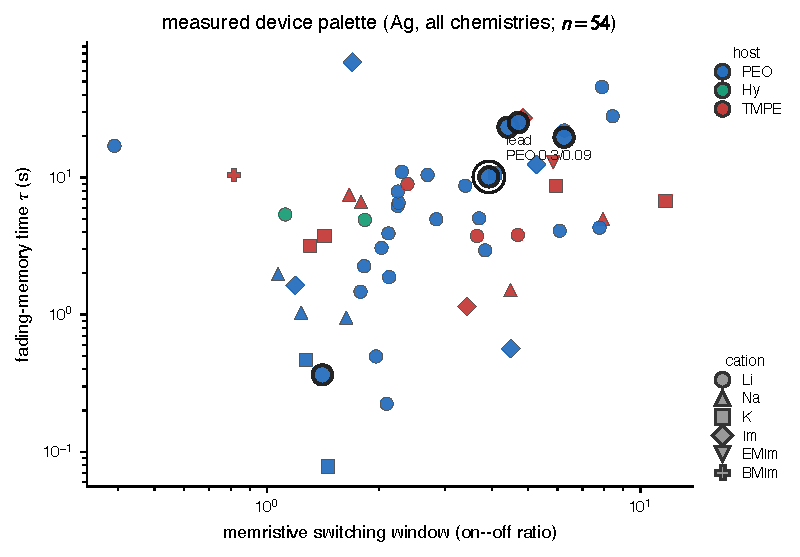
\includegraphics[width=0.82\linewidth]{../figures/chapter4/palette.pdf}
  \caption[Realised device palette across the library]{Measured window-versus-retention palette of the silver device library (\(n=54\) devices with both a clean hysteresis window and a fading-memory fit, all chemistries). Colour encodes the ion-conductor host, marker encodes the salt cation; the lead \PEO{}~0.3/0.09 cell is ringed. The cloud spans over a decade in each axis, and the lead-cell replicates alone span \(\tau\approx\SIrange{0.4}{20}{\second}\). Descriptive overview only; the quantitative claims of \cref{ch:comparative} rest on the replicated composition spine, not on this map.}
  \label{fig:ch4_palette}
\end{figure}

\section{Impedance: Equivalent Circuit and Per-Cell Values}\label{app:ch4_eis_detail}

\paragraph{Equivalent-circuit model.} Beyond the model-free Nyquist-apex
resistance used in \cref{sec:ch4_eis}, each spectrum was also summarised by the
bulk ionic resistance \(R_{\mathrm{ion}}\) of an equivalent circuit adapted from
the polymer light-emitting electrochemical cell analysis of Munar \textit{et
al.}~\cite{Munar2012}, in which a series cable term is placed in parallel with
(i) the semiconductor electronic branch (effectively open at \SI{0}{\volt}),
(ii) a geometric constant-phase element, and (iii) an ionic branch of two
interfacial double layers in series with \(R_{\mathrm{ion}}\). Two cautions
apply. First, the archive holds two automated fits of this circuit; the
freely-fitted one (with per-parameter error estimates) tracks composition
appreciably better than a more tightly bounded variant, and only the former is
used. Second, per-spectrum circuit fits are genuinely ill-conditioned --- an
independent refit confirms that several do not converge robustly --- so
\(R_{\mathrm{ion}}\) is reported only as corroboration of the model-free quantity,
never as a precise number. Both observables nonetheless fall steeply and
monotonically with \PEO{} fraction (\cref{tab:ch4_eis_by_cell}): the model-free
\(Z_{\mathrm{real}}^{\mathrm{apex}}\) at rank correlation \(-0.83\) against \PEO{}
on cell medians, the fitted \(R_{\mathrm{ion}}\) at \(-0.84\).

\begin{table}[t]
  \centering
  \caption[Per-cell impedance summaries]{Equilibrium (\SI{0}{\volt}-DC) impedance per composition cell, silver \SY{}/\PEO{}/\LiTf{}. \(Z_{\mathrm{real}}^{\mathrm{apex}}\): model-free real impedance at the Nyquist apex. \(R_{\mathrm{ion}}\): freely-fitted bulk ionic resistance (corroborative only). \(t_{1/2}\): independently measured fading-memory time, repeated from \cref{tab:ch4_decay_by_cell} for the co-decline of \cref{fig:ch4_eis}b. Em-dash: no matched decay.}
  \label{tab:ch4_eis_by_cell}
  \footnotesize
  \setlength{\tabcolsep}{6pt}
  \begin{tabular}{llrrr}
    \toprule
    \PEO{} & salt & \(Z_{\mathrm{real}}^{\mathrm{apex}}\,(\Omega)\) & \(R_{\mathrm{ion}}\,(\Omega)\) & \(t_{1/2}\,(\mathrm{s})\) \\
    \midrule
    0.15 & 0.045 & \num{2.5e8} & \num{2.3e7} & --- \\
    0.15 & 0.09  & \num{1.7e8} & \num{8.7e6} & --- \\
    0.15 & 0.18  & \num{1.0e8} & \num{8.4e6} & 22.4 \\
    0.3  & 0.045 & \num{5.3e7} & \num{4.0e5} & 15.8 \\
    0.3  & 0.09  & \num{1.3e8} & \num{1.0e6} & 19.2 \\
    0.3  & 0.18  & \num{9.9e7} & \num{4.9e5} & --- \\
    0.6  & 0.045 & \num{5.3e6} & \num{1.4e5} & 3.3 \\
    0.6  & 0.09  & \num{2.6e7} & \num{4.6e4} & 3.5 \\
    0.6  & 0.18  & \num{1.9e7} & \num{8.9e4} & 5.5 \\
    1.2  & 0.045 & \num{4.1e5} & \num{1.9e2} & 2.7 \\
    1.2  & 0.09  & \num{5.6e5} & \num{1.1e4} & 6.0 \\
    1.2  & 0.18  & \num{3.8e7} & \num{1.5e5} & 9.0 \\
    \bottomrule
  \end{tabular}
\end{table}

\section{Electrode-Contrast Per-Cell Values}\label{app:ch4_electrode_table}

\Cref{tab:ch4_electrode_by_cell} lists the per-cell behavioural metrics behind the
silver-versus-gold contrast of \cref{sec:ch4_electrode}, including the host-free
and salt-free negative controls that confirm both the ion-transport polymer and
the dissolved salt are required for the memristive response.

\begin{table}[t]
  \centering
  \caption[Electrode-contrast per-cell metrics]{Per-cell behavioural metrics by top electrode (active silver vs inert gold), at the lead composition \num{0.3}/\num{0.09}. On--off and normalised loop area from HYST; \(V_{\mathrm{act}}\) activation voltage (V); peak ratio and \(\alpha\) from PULSES; \(t_{1/2}\) from DELAYTIME (s). Em-dash: no clean decay/fit at that cell. ``none'' rows are host-free or salt-free negative controls.}
  \label{tab:ch4_electrode_by_cell}
  \footnotesize
  \setlength{\tabcolsep}{4pt}
  \begin{tabular}{llrrrrrr}
    \toprule
    Chemistry & Elec. & on--off & area & \(V_{\mathrm{act}}\) & peak & \(\alpha\) & \(t_{1/2}\) \\
    \midrule
    PEO/Li/OTf  & Ag & 3.25 & 0.33 & 2.38 & 123.5 & 0.89 & 19.2 \\
    PEO/Li/OTf  & Au & 2.00 & 0.12 & 2.74 & 29.4  & 0.45 & 87.2 \\
    TMPE/Li/OTf & Ag & 3.82 & 0.32 & 4.18 & 53.7  & 0.33 & 3.7 \\
    TMPE/Li/OTf & Au & 1.29 & 0.07 & 3.61 & 1.9   & 0.17 & --- \\
    TMPE/Na/OTf & Ag & 5.54 & 0.30 & 3.26 & 497.9 & 1.23 & 3.9 \\
    TMPE/Na/OTf & Au & 1.47 & 0.11 & 6.39 & ---   & ---  & --- \\
    TMPE/K/OTf  & Ag & 7.01 & 0.41 & 3.10 & 237.5 & 1.19 & 5.2 \\
    TMPE/K/OTf  & Au & 1.43 & 0.06 & 5.86 & ---   & ---  & --- \\
    TMPE/Na/TFSI& Ag & 1.76 & 0.10 & 2.38 & 25.1  & 0.46 & --- \\
    Hy/Li/OTf   & Ag & 1.41 & 0.06 & 1.61 & 25.2  & 0.39 & --- \\
    none/Li/OTf & Ag & 0.99 & 0.00 & 1.07 & ---   & ---  & --- \\
    TMPE/none   & Ag & 2.95 & 0.20 & 3.18 & 73.0  & 0.96 & --- \\
    none/none   & Au & 1.03 & 0.01 & 1.29 & 2.8   & ---  & --- \\
    \bottomrule
  \end{tabular}
\end{table}

%% ============================================================
%%  Appendix D — Chapter 5 (Temporal Computing) Supporting Info
%%
%%  \include'd from thesis.tex under \appendix. Documents the
%%  parameter-card sourcing and the simulation / read-out
%%  settings, so the in-silico results are reproducible from the
%%  measured archive without consulting the scripts.
%% ============================================================

\chapter{Supporting Information for Chapter~\ref*{ch:temporal}}\label{app:ch5_si}

This appendix documents how the behavioural-model parameter cards of
\cref{sec:ch5_model} are sourced from the measured archive, and lists the
simulation and read-out settings used across the three evidence tiers. Together
with the per-cell tables of \cref{app:ch4_celltables}, it makes the in-silico
results reproducible without consulting the analysis scripts
(\path{scripts/ch5_figures.py}, \path{scripts/ch5_physio_context.py},
\path{scripts/ch5_onset.py}).

\section{Parameter-Card Sourcing}\label{app:ch5_cards}

Each composition cell is reduced to a parameter card
$(\tau_c,\beta_c,\alpha_c,\text{peak}_c)$ that drives one reservoir node type. The
values are taken directly from the comparative fits, with no free re-tuning:
\begin{itemize}
  \item the fading-memory law $\lambda_c(\Delta t)=\exp[-(\Delta t/\tau_c)^{\beta_c}]$ uses the per-cell $(\tau_c,\beta_c)$ of \cref{tab:ch4_decay_by_cell}; for the few cells without an identified stretched fit, a single exponential reproducing the model-free half-life is used instead ($\tau_c=t_{1/2}/\ln 2$, $\beta_c=1$);
  \item the write nonlinearity uses the per-cell growth exponent $\alpha_c$ and peak enhancement of \cref{tab:ch4_pulses_by_cell};
  \item the device-to-device spread injected into each bank is the within-cell scatter of those same tables.
\end{itemize}
The heterogeneous banks of \cref{sec:ch5_benchmarks,sec:ch5_physio} span the
replicated \PEO{}/\LiTf{} composition cells of \cref{tab:ch4_decay_by_cell}
($\tau$ from $\approx 3$ to $\approx 26$\,s); the homogeneous control banks are
jittered copies of the lead cell \PEO{}~0.3/0.09 alone.

\section{Simulation and Read-out Settings}\label{app:ch5_settings}

\Cref{tab:ch5_settings} collects the settings used throughout
\cref{ch:temporal}. All read-outs are a single linear ridge regression; no
nonlinear decoder is used, so any demonstrated computation is attributable to the
device nodes rather than the read-out.

\begin{table}[t]
  \centering
  \caption[Reservoir simulation and read-out settings]{Simulation and read-out settings across the three evidence tiers of \cref{ch:temporal}. All banks are spatial banks of independent (non-recurrent) leaky nodes driven by randomly-masked input; all read-outs are linear ridge regression.}
  \label{tab:ch5_settings}
  \footnotesize
  \setlength{\tabcolsep}{5pt}
  \begin{tabularx}{\linewidth}{@{}>{\raggedright\arraybackslash}p{3.4cm}X@{}}
    \toprule
    Setting & Value \\
    \midrule
    Node model & $x^{(i)}_n=\lambda_i x^{(i)}_{n-1}+[\max(w_i u_n,0)]^{\alpha_i}$ (\cref{sec:ch5_model}) \\
    Read-out & single linear ridge regression \\
    Bank size $N$ & 24 (benchmarks); 48 (physiology/affect) \\
    Seeds & 10 random input/bank seeds; means $\pm$ SD reported \\
    Significance tests & paired Wilcoxon signed-rank over seeds (or subjects) \\
    Memory capacity & $\mathrm{MC}_k$ summed over lags, random uniform input \cite{Jaeger2002STM} \\
    NARMA & NARMA-10 system identification, NRMSE \cite{AtiyaParlos2000} \\
    Information-processing capacity & degree-1 (linear) + degree-2 (nonlinear), bounded by $N$ \cite{Dambre2012} \\
    Affective corpus & \WESAD{} chest signals, leave-one-subject-out over 15 subjects \cite{Schmidt2018WESAD} \\
    Streaming cadence & $\Delta t=\SI{1}{\second}$; reconstruction delays $1,3,8,20,45$\,s \\
    Affect scoring & class-balanced macro-F1 \\
    \bottomrule
  \end{tabularx}
\end{table}

\section{Continuous-Monitoring Stress Test}\label{app:ch5_robust}

The deployment-robustness result of \cref{sec:ch5_robust} (\path{scripts/ch5_onset.py})
is a continuous binary stress detector: at every $\Delta t = \SI{1}{\second}$ step the
read-out predicts stress (\WESAD{} label~2) versus not-stress (baseline and amusement
pooled), leave-one-subject-out, with the same single linear ridge read-out and
$15$-second causal label smoothing used in the streaming task. Four matched banks of
$N=24$ nodes are compared on identical input masks: the instantaneous input (no
memory), a memoryless bank (leak set to zero, dimensionality only), the homogeneous
lead-only bank, and the heterogeneous composition bank.

Sensor corruption is modelled by adding, to the per-subject scaled streams
(channels in $[0,1]$), independent Gaussian noise of standard deviation $\sigma$ at
every sample, plus sparse motion-artefact bursts (short windows of amplified noise at
a $1\%$ per-sample rate), clipped back to $[0,1]$; the same realisation is applied to
the training and held-out streams so the comparison isolates each architecture's
intrinsic noise tolerance. Robustness curves are seed-averaged over three bank/noise
seeds; the per-subject significance test at $\sigma=0.4$ is a paired Wilcoxon
signed-rank over the fifteen subjects. Reported metrics are the binary macro-F1, the
pooled false-alarm rate (fraction of not-stress steps called stress), and --- for
completeness, though they do not separate the banks --- the transition-window
macro-F1 (steps within $\pm\SI{20}{\second}$ of a label change) and the onset
detection latency (time to the first $\geq\SI{5}{\second}$ sustained stress call after
each onset).


%% ---- Unified bibliography ----
\printbibliography[heading=bibintoc, title={References}]

\end{document}
